%!TEX TS-program = pdflatex
% dissertation.tex -- main dissertation file
%
% Wisconsin dissertation template
% Copyright (c) 2008-2009 William C. Benton.  All rights reserved.
%
% This program can redistributed and/or modified under the terms
% of the LaTeX Project Public License Distributed from CTAN
% archives in directory macros/latex/base/lppl.txt; either
% version 1 of the License, or (at your option) any later version.
%
% This program includes other software that is licensed under the
% terms of the LPPL and the Perl Artistic License; see README for details.
%
% You, the user, still hold the copyright to any document you produce
% with this software (like your dissertation).
%

% Copyright (c) 2013 Evan Driscoll
%
% In my evaluation the items remaining from Will's original version do not
% withstand the test of copyright, and so as a result I don't think I need to
% meet the sole criteria of the Latex PPL which I otherwise wouldn't -- I am
% not renaming this file.

%%% You'll want ``oneside'' for the deposit version, but probably not for any
%%% versions that don't need to meet the UW requirements
%\documentclass[12pt,letterpaper,numbers,oneside]{memoir}
%\documentclass[12pt,letterpaper,numbersm,oldfontcommands]{memoir}
\documentclass[12pt, letterpaper, oldfontcommands]{memoir}

%\def\ShortenThesis{y}

%\newcommand{\TODO}[1]{\textbf{#1}\protect\marginnote{\large{[**]}}}
\newcommand{\CHECK}[1]{#1} %\protect\marginnote{\large{[**]}}}

\input{includes/preamble}
\input{includes/defs}

\usepackage[algo2e,noline,noend,linesnumbered,algochapter]{algorithm2e}
\usepackage{algorithmic} % must come after hyperref
\usepackage{algorithm}
\usepackage{aliascnt}
\usepackage{bookmark}
\usepackage{mathtools}
\usepackage{colortbl}
\usepackage{lipsum}
%\usepackage[hyphens]{url}
\PassOptionsToPackage{hyphens}{url}
% Include last: only autonum should be after this (or hypdvips, but if you
% need that you're doing something wrong)
\usepackage[capitalize]{cleveref}

\usepackage{alltt,url}
\usepackage{rotating}
%\usepackage{textcomp}
%\usepackage{graphics}
%\usepackage{floatflt}
\usepackage{multirow}
%\usepackage{cite}
%\usepackage{needspace}
%\usepackage[hyphens, breaklinks]{hyperref}
%\usepackage{breakurl}
\usepackage{hyperref}
%\usepackage{epstopdf}
%\epstopdfDeclareGraphicsRule{.eps}{pdf}{.pdf}{%
%ps2pdf -dEPSCrop #1 \OutputFile
%}
\usepackage{fancyvrb}
\usepackage{relsize}
\usepackage{soul}
\usepackage{array}
\usepackage{caption}

\usepackage{graphicx} % for subfigure
%\newsubfloat{figure} % for subfigure 

%\usepackage{subfigure}
%\usepackage{subcaption}
%\captionsetup{compatibility=false}
%\captionsetup[subfigure]{labelformat=simple, labelsep=colon}
%\captionsetup[subfloat]{labelfont={bf,small},textfont={it,small},
%subrefformat=parens}

\usepackage{booktabs}
\usepackage{enumitem}
\usepackage{verbatim}
%\usepackage[toc,page]{appendix}
%%%%%%%%%%%%%%%%%%
\usepackage{caption}
\usepackage{subcaption}
\usepackage{multirow}
\usepackage{amssymb}% http://ctan.org/pkg/amssymb
\usepackage{pifont}% http://ctan.org/pkg/pifont
\usepackage{cleveref}
%%%%%%%%%%%%%%%%%%%%

\newlength{\tmpa}
\newlength{\tempa}



% haryadi .. parskip, and parindent
%\setlength\parindent{0pt}
%\setlength\parskip{5pt}


\newcommand{\beforesec}{\vspace{-.4cm}}
\newcommand{\aftersec}{\vspace{-.3cm}}

\newcommand{\beforesect}{\vspace{-.1cm}}
\newcommand{\aftersect}{\vspace{-.3cm}}

\newcommand{\beforesub}{\vspace{-.3cm}}
\newcommand{\aftersub}{\vspace{-.25cm}}

\newcommand{\beforesubsub}{\vspace{-.2cm}}
\newcommand{\aftersubsub}{\vspace{-.2cm}}

 \newcommand{\zsubsection}[1]{\section{#1}}
 \newcommand{\zsubsubsection}[1]{\subsection{#1}}
 \newcommand{\zsubsubsubsubsection}[1]{\subsubsection{#1}}

\newcommand{\smush}{0.25in}

\newcommand{\figWidthOne}{3.05in} 
\newcommand{\figWidthHalf}{1.45in} 
\newcommand{\figWidthTwo}{3.05in} 
\newcommand{\figWidthTwop}{1.6in} 
%\newcommand{\figWidthThree}{2.65in} 
\newcommand{\figWidthThree}{2.2in} 
\newcommand{\figWidthSix}{1.1in} 
\newcommand{\figWidthFour}{1.7in} 
\newcommand{\figHeight}{2.0in}
\newcommand{\captionText}[2]{\textbf{#1} \textit{\small{#2}}}

\newcommand{\zbullet}{\hspace{-0.1cm}$\bullet$}

\newcommand{\eg}{\textit{e.g.},~}
\newcommand{\ie}{\textit{i.e.},~}
\newcommand{\etal}{\textit{et al.}}
\newcommand{\apriori}{\textit{a priori}}

%-------------------------------------------------------------------
% haryadi -- new command
\newcommand{\msub}[1]{\vspace{1pt}\noindent{\bf #1}}

\newcommand{\ts}[1]{{\tt{\small#1}}}
\newcommand{\tsb}[1]{{\tt{\small{\bf#1}}}}
\newcommand{\tse}[1]{{\tt{\small{\em#1}}}}
\newcommand{\tss}[1]{{\tt{\footnotesize#1}}}
\newcommand{\exc}{$^{\ddag}$}        % except
\newcommand{\EIO}{\ts{EIO}}

%-------------------------------------------------------------------
% For reliability table
\newcommand{\ip}{bad}
\newcommand{\nullp}{$\emptyset$}

\newcommand{\oops}{o}
\newcommand{\dead}{$\times$}
\newcommand{\alive}{$\surd$}
\newcommand{\unuse}{$\times$}

% Detected or undetected column
\newcommand{\detected}{$\surd$}
\newcommand{\undetected}{$\times$}

% Blocks dropped column
\newcommand{\childinode}{C$^{inode}$}  % child inode
\newcommand{\parentdir}{P$^{dir}$}  % parent dir
\newcommand{\childdir}{C$^{dir}$}  % child dir
\newcommand{\olddir}{O$^{dir}$}  % old parent dir
\newcommand{\newdir}{N$^{dir}$}  % new parent dir
\newcommand{\childdata}{C$^{data}$}  % child data block
\newcommand{\childinddata}{C$^{ind}$}  % child indirect block
\newcommand{\firstinode}{O$^{inode}$}  % child indirect block

% Error column
\newcommand{\parentdirbad}{P$^{BD}$}  % Bad dir entry for parent
\newcommand{\orphanblock}{C$^{OB}$}  % Orphan block
\newcommand{\orphaninode}{C$^{OI}$}  % Orphan inode
\newcommand{\childdirbad}{C$^{BD}$}  % Bad dir entry for child
\newcommand{\olddirbad}{O$^{BD}$}  % Bad dir entry for old inode
\newcommand{\childinodeincon}{C$^{HL}$}  % Inconsistency in child inode hardlinks
\newcommand{\sechole}{$\ast$}  % Inconsistency in child inode hardlinks
\newcommand{\garbage}{C$^{GD}$}  % Garbage data
\newcommand{\stalepointer}{O$^{TP}$}  % A has a wrong pointer to a block

%Corrective action
\newcommand{\childinodeerror}{C$^{EI}$}  % Error on accessing child inode
\newcommand{\reclaim}{R}  % Reclaimed on scan
\newcommand{\childdirerror}{C$^{ED}$}   % Error on child dir access
\newcommand{\childblockerror}{C$^{EB}$}   % Error on child block access
\newcommand{\newdirerror}{C$^{EN}$}   % Error on child dir access via new path
\newcommand{\olddirerror}{C$^{EO}$}   % Error on child dir access via old path
\newcommand{\newreaderror}{O$^{ER}$}   % Error on inode A's read access
\newcommand{\none}{--}  % Reclaimed on scan
\newcommand{\oldblockerror}{O$^{EB}$}   % Error on block access in old file

\newcommand{\use}{$\surd$}
\newcommand{\ic}{$\times$}
\newcommand{\con}{$\surd$}
\newcommand{\gpf}{G}
\newcommand{\npe}{null-pointer}
\newcommand{\usebuta}{$\surd^a$} % unmountable
\newcommand{\hwdetect}{d}

%% TABLE 2
\newcommand{\lateoops}{o$^b$}  % oops happens, but late
\newcommand{\lategpf}{G$^b$}   % gpf, but late
\newcommand{\iop}{i}           % invalid opcode
\newcommand{\detects}{d}       % assertion
\newcommand{\silentret}{s}     % app fails silently
\newcommand{\errorret}{e}      % app returns an error
\newcommand{\appworks}{$\surd$}     % app works!
\newcommand{\usebutar}{$\surd^{ar}$} % read-only and unmountable

\newcommand{\tbls}{\hspace{0.025in}}
\newcommand{\tblss}{\hspace{0.015in}}
\newcommand{\shrinkless}{\vspace{-0.01cm}}

%-------------------------------------------------------------------

%-------------------------------------------------------------------

% axes         
\newcommand{\x}{{\em x}}
\newcommand{\y}{{\em y}}
\newcommand{\xaxis}{x-axis}
\newcommand{\yaxis}{y-axis}

\newcommand{\KB}{~KB}
\newcommand{\KBs}{~KB/s}
\newcommand{\Kbs}{~Kbit/s}
\newcommand{\mbs}{~Mbit/s}
\newcommand{\MB}{~MB}
\newcommand{\GB}{~GB}
\newcommand{\MBs}{~MB/s}
\newcommand{\mus}{\mbox{$\mu s$}}
\newcommand{\ms}{\mbox{$ms$}}


\newcommand{\unix}{{\sc Unix}}
%\newcommand{\NULL}{{\sc NULL}}

\newcommand{\bquote}{\vspace{-0.25cm} \begin{quote}}
\newcommand{\equote}{\end{quote}\vspace{-0.05cm} }

\newcommand{\zquote}[2]{\begin{quote}
#1 --
{\em``#2'' }
%{\bf -- #1 }
\end{quote}}


\newcommand{\XXX}[1]{{\small {\bf (XXX: #1)}}}

\newcommand{\XXXX}{{\bf XXX}}
\newcommand{\xx}{{\bf XXX}}

% Image caption distance
\if 0
\newcommand{\beforecaption}{\vspace{-.35cm}\begin{spacing}{0.80}}
\newcommand{\aftercaption}{\vspace{-.5cm}\end{spacing}}
\newcommand{\mycaption}[3]{{\tiny \beforecaption\caption{\label{#1}{#2} {\em #3}}\aftercaption}}
\fi

% normal
\newcommand{\beforecaption}{\begin{spacing}{0.90}}
\newcommand{\aftercaption}{\end{spacing}}
\newcommand{\mycaption}[3]{{\beforecaption\caption{\label{#1}{\bf #2. } {\em \small #3}}\aftercaption}}


% osdi06
\if 0
\newcommand{\beforecaption}{\vspace{-.25cm} \begin{spacing}{0.80}}
\newcommand{\aftercaption}{\vspace{-.1cm} \end{spacing}}
\newcommand{\mycaption}[3]{{\beforecaption\caption{\label{#1}{\bf #2. } {\em \footnotesize #3}}\aftercaption}}
\fi

\if 0
\newcommand{\beforecaption}{\begin{spacing}{0.80}}
\newcommand{\aftercaption}{\end{spacing}\vspace{-.3cm}}
\newcommand{\mycaption}[3]{{\beforecaption\caption{\label{#1}{\small \bf #2} {\footnotesize \em #3}}\aftercaption}}
\fi


\newcommand{\sref}[1]{\S\ref{#1}}

\newcommand{\xxx}[1]{  \underline{ {\small {\bf (XXX: #1)}}}}


\newenvironment{packeditemize}{
\begin{itemize}
  \setlength{\itemsep}{1pt}
  \setlength{\parskip}{0pt}
  \setlength{\parsep}{0pt}
}{\end{itemize}}

\newcommand{\pincon}{$P_{inc}$}
\newcommand{\pin}{$P_{inc}$}
\newcommand{\pinmath}{P_{inc}}
\newcommand{\dt}{$T_{D}$}

\if 0
\newcommand{\sysfsync}{\texttt{\fontsize{9.2}{5}\selectfont fsync()}}
\newcommand{\syscsync}{\texttt{\fontsize{9.2}{5}\selectfont osync()}}
\newcommand{\sysdsync}{\texttt{\fontsize{9.2}{5}\selectfont dsync()}}
\newcommand{\sysrename}{\texttt{\fontsize{9.2}{5}\selectfont
    rename()}}
\newcommand{\fsync}{\sysfsync}
\newcommand{\writec}{\texttt{\fontsize{9.2}{5}\selectfont write()}}
\newcommand{\gedit}{{\fontsize{9.2}{5}\selectfont gedit}}
\fi

\newcommand{\sysfsync}{\texttt{fsync()}}
\newcommand{\syscsync}{\texttt{osync()}}
\newcommand{\sysdsync}{\texttt{dsync()}}
\newcommand{\sysrename}{\texttt{rename()}}
\newcommand{\fsync}{\sysfsync}
\newcommand{\writec}{\texttt{write()}}
\newcommand{\gedit}{\texttt{gedit}}
\newcommand{\sataflush}{\texttt{FLUSH}}

\newcommand{\smalltt}[1]{\texttt{#1}}
\newcommand{\fstoolname}{\textsc{Bob}}
%\newcommand{\toolname}{\mbox{\textsc{Alice}}}

\if 0
\newcommand{\detected}{$\surd$}
\newcommand{\undetected}{$\times$}
\fi

% Stuff from the OSDI paper, shouldn't need all of these.
\newcommand{\fwrong}{$\times$}
\newcommand{\verysmalltt}[1]{\texttt{\scriptsize #1}}
\newcommand*\rot{\rotatebox{90}}
\newcommand{\Kassandra}{Kassandra}
\newcommand{\microprogram}{microprogram}
\newcommand{\microprograms}{microprograms}
\newcommand{\microinstruction}{microinstruction}
\newcommand{\microinstructions}{microinstructions}
\newcommand{\Microinstructions}{Microinstructions}
\newcommand{\writeSC}{\smalltt{write()}}
\newcommand{\fsyncSC}{\smalltt{fsync()}}
\newcommand{\msyncSC}{\smalltt{msync()}}
\newcommand{\fdatasyncSC}{\smalltt{x fdatasync()}}
\newcommand{\linkSC}{\smalltt{link()}}
\newcommand{\mkdirSC}{\smalltt{mkdir()}}
\newcommand{\fempty}{$\phi$}
\newcommand{\fexists}{$\surd$}
\newcommand{\creatSC}{{\smalltt{creat()}}}
\newcommand{\unlinkSC}{{\smalltt{unlink()}}}
\newcommand{\renameSC}{{\smalltt{rename()}}}

\newcommand{\totbugs}{60}
\newcommand{\totapps}{11}
\newcommand{\totappsw}{eleven}


\newcommand{\ifs}{IceFS}
\newcommand{\toolname}{WiscKey}


%%%%%%%%%%%%%%%%%%%%%%%%%%%%%%%%%%%%%
%% No \usepackage after this point %%
%%%%%%%%%%%%%%%%%%%%%%%%%%%%%%%%%%%%%

\input{includes/thesisdefs}

% Some style options
\hangcaption
\captionnamefont{\small}
\captiontitlefont{\small}

\setsecnumdepth{subsection}
\maxtocdepth{subsection}

\crefname{algorithm}{Listing}{Listings}
\Crefname{algorithm}{Listing}{Listings}
\crefname{equation}{Equation}{Equations}

%%%%%%%%%%%%%%%%%%%%%%%%%%%%%%%%%%%%%%%%%%%
%% Number tables, theorems, and listings %%
%% inline with figures,  instead of with %%
%% their own,  parallel counter which is %%
%% dumb.                                 %%
%%%%%%%%%%%%%%%%%%%%%%%%%%%%%%%%%%%%%%%%%%%
\makeatletter
\let\c@table\@undefined
\let\c@thm\@undefined
\let\c@algocf\@undefined
\makeatother

\newaliascnt{table}{figure}
\newaliascnt{thm}{figure}
\newaliascnt{algocf}{figure}
%%%%%%%%%%%%%%%%%%%%%%%%%%%%%%%%%%%%%%%%%%%%

\renewcommand{\AlCapSty}[1]{#1}
\renewcommand{\AlCapFnt}{\small}
\renewcommand*{\cftfigurename}{Figure\space}

\renewcommand*{\cftfigurename}{Figure\space}
\renewcommand*{\cfttablename}{Table\space}
%\newcommand*{\cftalgocfname}{Listing\space}


%%%%%%%%%%%%%%%%%%%%%%%%%%%%%%%%%%%%%%%%%%%%

\newcommand{\algrule}[1][.2pt]{\par\vskip.2\baselineskip\hrule height #1\par\vskip.2\baselineskip}
\newcommand{\cf}{{cf.}\xspace}

\newcommand{\cut}[1]{}

\renewcommand{\ttdefault}{cmtt}
\newcommand{\tightparagraph}[1]{\vspace{5pt}\noindent\textbf{#1}\ }

\newcommand{\acdc}{{AC/DC}\xspace}
%\newcommand{\acdc}{{AC/DC}\xspace}
\newcommand{\cwnd}{{{\tt CWND}}\xspace}
\newcommand{\rwnd}{{{\tt RWND}}\xspace}
\newcommand{\crs}[1]{#1}% Do nothing
%\usepackage{cleveref}
\crefname{section}{§}{§§}
\Crefname{section}{§}{§§}
\crefformat{section}{§#2#1#3}

%%%%%rate limiter
\newcommand{\dem}{DEM\xspace}
\newcommand{\spring}{SPRING\xspace}
\newcommand{\nameone}{DEM\xspace}
\newcommand{\nametwo}{SPRING\xspace}
\newcommand{\cmark}{\ding{51}}%
\newcommand{\xmark}{\ding{55}}

%%%%%%%%%%%%%%%%%%%%%%%%%%%%%%%%%%%%%%%%%%%%

\overfullrule=2mm

% Thesis options
\title{Improving Datacenter Network Performance via Intelligent Network Edge}
\author{Keqiang He}
\department{Computer Sciences}
\date{2017 \vspace{-1in}}

\defensedate{June 8, 2017}
\committeeMemberOne{Aditya Akella, Professor, Computer Sciences}
\committeeMemberTwo{Suman Banerjee, Professor, Computer Sciences}
\committeeMemberThree{Eric Rozner, Research Staff Member, IBM Research}
\committeeMemberFour{Michael Swift, Associate Professor, Computer Sciences}
\committeeMemberFive{Xinyu Zhang, Assistant Professor, Electrical \& Computer Engineering}

\includeonly{frontmatter/fm,xfa-pcca}

\begin{document}

% Add \part declarations if you want, but it's not necessary
%\part{Preliminaries}

\ifdef{\ShortenThesis}{
}{
  \hypersetup{pageanchor=false}

%% http://tex.stackexchange.com/questions/18924/pdftex-warning-ext4-destination-with-the-same-identifier-nam-epage-1-has
\maketitle

\advisorname{Aditya Akella}
\advisortitle{Professor}

% TODO: ABSTRACT
\begin{umiabstract}
  \begin{abstract}

A lot of recent work has been focusing on solving in network latency in datacenter networks. 
In this paper, we focus on a less explored topic \textemdash\xspace latency 
increase caused by rate limiters on the end-host. 
We show that latency can be increased by an order of magnitude 
by the rate limiters in cloud networks, 
and simply extending ECN into rate limiters is not sufficient. 
To this end, we propose two techniques \textemdash\xspace~\dem{} and~\spring{} to improve the performance of rate limiters. 
Our experiment results demonstrate that~\dem{} and~\spring{} enabled 
rate limiters can achieve high (and stable) throughput and low latency.

\iffalse
Bandwidth guarantee is an essential feature to satisfy tenants' QoS requirement in clouds. However, its token-buffer-based implementation is not compatible with other aspects of QoS, i.e., latency and packet loss. In this paper, we propose to \name, which guarantees bandwidth allocation, low latency and little packet loss. The main idea is to maintain a large token buffer to tolerate traffic burst and keep low buffer occupancy to obtain low queuing latency. The low occupancy is achieved by carefully adjust traversing flows' sending rate. We implement \name in two ways for different virtualized environments: 
(1) adjust flows' congestion window directly at token buffers according to instantaneous queue length, which suits VM-based clouds,  (2) enable ECN at token buffers and leverage DCTCP for congestion control at end points, which suits container-based clouds. We integrate \name into a widely used virtual switch \textemdash\xspace OVS, so that \name can be deployed without any changes to OS kernels. And our evaluation shows \wenfei{result}.

\fi

\end{abstract}

\end{umiabstract}


%%% SOME OF THIS CODE IS ADAPTED FROM THE VENERABLE withesis.cls

% COPYRIGHT PAGE
%  - To include a copyright page use \copyrightpage
%\copyrightpage
%\thispagestyle{empty}

\chapterstyle{jenor}
% TODO: DEDICATION
\begin{dedication}
  \pagenumbering{roman} % This makes the page numbers Roman (i, ii,
                        % etc)
  \setcounter{page}{3}
  \hypersetup{pageanchor=true} \emph{To my family}
\end{dedication}

%% BEGIN PAGESTYLE

%%% You can pick a pagestyle if you want; see the memoir class
%%% documentation for more info.  The default ``deposit'' option meets
%%% the UW thesis typesetting requirements but is probably
%%% unsatisfactory for making a version of your dissertation that
%%% won't be deposited to the graduate school (e.g. for web or a nice
%%% printed copy)


% TODO: ACKNOWLEDGMENTS
\begin{acks}

Life is short, especially when you decide to pursue a PhD. How to
spend time wisely always puzzles me. Looking into the mirror, I am not
young anymore, but I feel very lucky for my stubborn decision and a
humble dream several years ago. Now, my school life almost ends. An
ending is also a new beginning. At this crossroad, let me thank those 
who have helped me both in work and life. 

% remzi and andrea
First, I would like to thank my advisors Remzi and Andrea
Arpaci-Dusseau. Before I worked with them, I was a frustrating
graduate student. They patiently helped me for many years to achieve
my research dream, including how to find a great 
problem, how to get inspiration, how to think deeply, how 
to communicate clearly, how to write a good paper, and how to do a
great presentation. I remember that they provided detailed suggestions
slide by slide in numerous late afternoon group meetings. I remember
many inspirational quotes from them: ``Double your reading sources'',
``Such is life'', ``We should target a best paper''. I remember that
they met me at Google Madison and Palo Alto downtown to listen to my
random ideas at random time. Remzi even taught me how to embed a joke
in my conference presentation. Doing research with them becomes easy,
fun and meaningful. 

I also learned a lot from their personalities. I was seriously sick
and rested at home for nearly one semester. I remember that Remzi
emailed me every Monday morning to ask what he can help. He offered to
talk to my doctor to make sure I was treated well. Remzi's great sense
of humor urged me to buy a book about how to have a sense of
humor. Andrea always smiles. She constantly encourages me and shares 
her confidence in my projects, especially during the hard time and the
deadline rush. They share their first-class OS book online for free,
making me rethink the value of money. Even though I decided to join
industry, they helped me greatly by connecting me with their friends
in many companies, and taught me how to negotiate offers wisely. What
else can you ask for? 

% thesis committee 
I would also like to thank my thesis committee. Shan Lu is also a
coauthor of my first paper here. I remember that she sat with me to
read many file system bug patches, and taught me different types of
concurrency bugs. She is willing to help when I need a recommendation
letter at various occasions. It is lucky to have Michael Swift as my
prelim and thesis committee. He is very rigorous and his extensive
questions, comments and feedback on different parts of my thesis
helped make it much better. I also thank Xinyu Zhang for reading my
thesis and giving me good suggestions. 

% internship mentors
I have been fortunate to do excellent internships throughout my PhD. 
I would like to thank the companies as well as my mentors there: 
Prasenjit Sarkar, Dinesh Subhraveti, Dean Hildebrand and Renu Tewari
at IBM; Herodotos Herodotou, Sriram Rao and Raghu Ramakrishnan at
Microsoft; Asit Desai and Sunil Satnur at VMWare. Working with these
people have been a great and rewarding experience for me. 

% colleagues
I am fortunate to work and discuss with a group of high quality
students here: Yupu Zhang, Thanumalayan Pillai, Thanh Do, Jun He,
Vijay Chidambaram, Yiying Zhang, Zev Weiss, Tyler Harter, Ao Ma,
Asim Kadav, Suli Yang, Chris Dragga, Leo Arulraj, Ramnatthan
Alagappan, Sriram Subramanian, and Swami Sundararaman. In particular,
I would like to thank my coauthors Yupu, Thanu and Thanh. Yupu is
always ready to discuss design and implementation details, help coding
and write the paper. Thanu's expertise in crash consistency and
hacking skills amazed me. Thanh gave me lots of great advice in
research and life. I also want to thank my officemate Vijay, who is
always full of motivation and curiosity. Having Thanu and Vijay as
officemates definitely helped me a lot to be a better researcher.  

% friends
I am grateful to have many friends at Madison to make my life more
interesting. I thank Ji Liu for being a great roommate when I arrived 
Madison. I thank the Shell Friday basketball team for numerous fun
games and great memories every Friday afternoon. I thank Wenbin Fang
and Jun He for inviting me to many delicious dinners at their homes. I 
thank Yvonne Koh for practicing English speaking with me patiently in
her free time. I also would like to thank many other friends at CS:
Jia Xu, Yinan Li, Linhai Song, Guoliang Jin, Wenfei Wu, Qian Wan,
Yimin Tan, Junming Xu, Yeye He, and Tan Zhang. With you all, the PhD
journey is not lonely anymore.   

% family
In closing, I turn towards family. I would like to thank my
parents for their unconditional love and support. They raised me in an
environment with an emphasis on education and good personality. They
set good examples for me in both work and life with their hard work 
and kindness. I have left home for study since I was 14. In these past
years, my parents always supported me to pursue my dreams, no matter how
far I will go and how long I will take. I remember that my mother
cried every time when I left home for high school, college and
graduate school. I remember my father woke me up and jogged with me
in the hills nearly every morning when I was home. Their love enables
me to go forward fearlessly. Finally, I thank my wife Xin for
her love since we met. She took care of me in many ways even though she is also
busy with her own research and study. I remember she cooked countless 
delicious meals for me when I work for various deadlines. She always
supports me, cheers me up and helps me to be a better person. I
dedicate this dissertation to my family: mother, father and Xin.  

\end{acks}

% CONTENTS, TABLES, FIGURES

%\makeatletter
%\renewcommand{\@pnumwidth}{1}
%\makeatother

\renewcommand{\printtoctitle}[1]{\chapter*{#1}}
\renewcommand{\printloftitle}[1]{\chapter*{#1}}
\renewcommand{\printlottitle}[1]{\chapter*{#1}}

%\renewcommand{\cftchapteraftersnumb}{\\}
%\cftsetindents{chapter}{0em}{0em}
\renewcommand{\cftchapterfont}{\bfseries}
\renewcommand{\cftchapterpagefont}{\bfseries}
\renewcommand{\cftchapterpresnum}{\bfseries}
%\renewcommand{\cftchapterleader}{} 
%\renewcommand{\cftchapterafterpnum}{\cftparfillskip} 

\renewcommand{\tocmark}{}
\renewcommand{\lofmark}{}
\renewcommand{\lotmark}{}

\renewcommand{\tocheadstart}{}
\renewcommand{\lofheadstart}{}
\renewcommand{\lotheadstart}{}

\renewcommand{\aftertoctitle}{}
\renewcommand{\afterloftitle}{}
\renewcommand{\afterlottitle}{}

\cftpagenumbersoff{part}
\renewcommand{\cftpartpresnum}{}
%\renewcommand{\cftdotsep}{\cftnodots}
\makeatletter
\renewcommand*\l@part[2]{%
  \ifnum \c@tocdepth >-2\relax
    \addpenalty{-\@highpenalty}%
    \addvspace{2.25em \@plus\p@}%
    \setlength\@tempdima{3em}%
    \begingroup
      \parindent \z@ \rightskip \@pnumwidth
      \parfillskip -\@pnumwidth
      {\leavevmode
       \hspace*{\fill}\centering\Large\bfseries{}Part$\ \ $\smash[b]{#1}\hspace*{\fill}}%
       \vspace{1.3ex}\hrule\par%
       \nobreak
         \global\@nobreaktrue
         \everypar{\global\@nobreakfalse\everypar{}}%
    \endgroup
  \fi}
\makeatother

\renewcommand{\cftsectionfont}{}
\renewcommand{\cftsectionpagefont}{\itshape}
\renewcommand{\cftsectionleader}{\hspace{0.8em}}
\renewcommand{\cftsectionafterpnum}{\cftparfillskip} 

\renewcommand{\cftsubsectionleader}{\hspace{0.8em}}
\renewcommand{\cftsubsectionpagefont}{\itshape}
\renewcommand{\cftsubsectionafterpnum}{\cftparfillskip} 

% \captionnamefont{\small\sffamily} 
% \captiontitlefont{\small\sffamily} 

% \renewcommand{\contentsname}{contents}
% \renewcommand{\listfigurename}{list of figures}
% \renewcommand{\listtablename}{list of tables}

\makeatletter
  \renewcommand\ext@table{lof}
  \renewcommand\ext@algocf{lof}

  \newlength{\cftbeforealgocfskip}
  \setlength{\cftbeforealgocfskip}{\cftbeforefigureskip}
  \newlength{\cftalgocfindent}
  \setlength{\cftalgocfindent}{\cftfigureindent}
  \newlength{\cftalgocfnumwidth}
  \setlength{\cftalgocfnumwidth}{\cftfigurenumwidth}

  \newcommand{\cftalgocffont}{\cftfigurefont}
  \newcommand{\cftalgocfname}{Listing }
  \newcommand{\cftalgocfpresnum}{\cftfigurepresnum}
  \newcommand{\cftalgocfaftersnum}{\cftfigureaftersnum}
  \newcommand{\cftalgocffillnum}{\cftfigurefillnum}

  \renewcommand*\l@algocf[2]{%
     \ifnum \@nameuse {c@lofdepth} > 0\relax \vskip%
            \@nameuse {cftbeforealgocfskip}%
            {%
               \newcommand *\cftwhatismyname {algocf}\memRTLleftskip \@nameuse {cftalgocfindent}\relax%
               \memRTLrightskip \@tocrmarg \parfillskip -\memRTLrightskip \parindent%
               \@nameuse {cftalgocfindent}\relax \@afterindenttrue \interlinepenalty \@M \leavevmode%
               \settowidth {\@tempdima }%
               {%
                   \@nameuse {cftalgocffont}\@nameuse {cftalgocfname}%
               }%
               \addtolength {\@tempdima }{\@nameuse {cftalgocfnumwidth}}%
               \expandafter \let \expandafter \@cftbsnum \csname cftalgocfpresnum\endcsname%
               \expandafter \let \expandafter \@cftasnum \csname cftalgocfaftersnum\endcsname%
               \expandafter \let \expandafter \@cftasnumb \csname cftalgocfaftersnumb\endcsname%
               \expandafter \let \expandafter \@cftn@me \csname cftalgocfname\endcsname%
               \advance \memRTLleftskip \@tempdima \null \nobreak \hskip -\memRTLleftskip%
               {%
                   \@nameuse {cftalgocffont}#1%
               }\nobreak%
               \@nameuse {cftalgocffillnum}{#2}%
           }%
      \fi}

%  \renewcommand*\listfigurename{List of Figures, Tables, and Listings}
  \renewcommand*\listfigurename{List of Figures and Tables}
\makeatother

\newlength\figlen
\settowidth\figlen{Figure}
\newlength\tablen
\settowidth\tablen{Table}
\newlength\lstlen
\settowidth\lstlen{Listing}

\newlength\FigNumSpace
\newlength\TabNumSpace

\addtolength\TabNumSpace{\lstlen - \tablen}
\addtolength\FigNumSpace{\lstlen - \figlen}

\renewcommand*{\cftfigurename}{Figure \hspace{\FigNumSpace}}
\renewcommand*{\cfttablename}{Table \hspace{\TabNumSpace}}
\renewcommand*{\cftalgocfname}{Listing }


\tableofcontents

\clearpage
\listoffigures

\clearpage
% NOMENCLATURE
% \begin{conventions}
% % \begin{description}
% % \item{\makebox[0.75in][l]{term}
% %        \parbox[t]{5in}{definition\\}}
% % \end{description}
% \input{conventions}
% \end{conventions}

% TODO abstract
\if 0
\begin{abstract}
  \begin{abstract}

A lot of recent work has been focusing on solving in network latency in datacenter networks. 
In this paper, we focus on a less explored topic \textemdash\xspace latency 
increase caused by rate limiters on the end-host. 
We show that latency can be increased by an order of magnitude 
by the rate limiters in cloud networks, 
and simply extending ECN into rate limiters is not sufficient. 
To this end, we propose two techniques \textemdash\xspace~\dem{} and~\spring{} to improve the performance of rate limiters. 
Our experiment results demonstrate that~\dem{} and~\spring{} enabled 
rate limiters can achieve high (and stable) throughput and low latency.

\iffalse
Bandwidth guarantee is an essential feature to satisfy tenants' QoS requirement in clouds. However, its token-buffer-based implementation is not compatible with other aspects of QoS, i.e., latency and packet loss. In this paper, we propose to \name, which guarantees bandwidth allocation, low latency and little packet loss. The main idea is to maintain a large token buffer to tolerate traffic burst and keep low buffer occupancy to obtain low queuing latency. The low occupancy is achieved by carefully adjust traversing flows' sending rate. We implement \name in two ways for different virtualized environments: 
(1) adjust flows' congestion window directly at token buffers according to instantaneous queue length, which suits VM-based clouds,  (2) enable ECN at token buffers and leverage DCTCP for congestion control at end points, which suits container-based clouds. We integrate \name into a widely used virtual switch \textemdash\xspace OVS, so that \name can be deployed without any changes to OS kernels. And our evaluation shows \wenfei{result}.

\fi

\end{abstract}

\end{abstract}
\fi

\clearpage\pagenumbering{arabic}

%%% END STUFF TAKEN FROM WITHESIS EXAMPLE FILE

\renewcommand{\partnumfont}{\fontfamily{pbk}\fontseries{m}\fontshape{n}%
    \fontsize{0.8in}{0in}\selectfont\raggedright\textcolor[rgb]{.44,.59,.77}}

\renewcommand{\partnamefont}{\fontfamily{pbk}\fontseries{m}\fontshape{n}%
    \fontsize{0.8in}{0in}\selectfont\raggedright\textcolor[rgb]{.44,.59,.77}}

\renewcommand{\parttitlefont}{\fontfamily{pbk}\fontseries{m}\fontshape{n}%
    \fontsize{0.38in}{0in}\selectfont\raggedright}

\renewcommand{\beforepartskip}{\thispagestyle{deposit}}
\renewcommand{\midpartskip}{\par\vspace{1in}}

}

\chapter{Introduction}
\label{thesis:chapter:intro}
\chapter{Introduction}
\label{chap:intro}
Over the past few years, cloud-based networking solutions have been gaining widespread acceptance and
deployment for organizations such as enterprises and institutions. 
Today's data centers are infrastructures of various services, including search, content distribution,
big data analysis, and virtual networks. The cloud providers obtain revenue by multiplexing the 
infrastructure among the cloud tenants and the tenants save the trouble of needing to manage the network by themselves.
Recent studies have forecast that global data center traffic (both inter and intra) in 2018 will 
be triple the traffic in 2013~\cite{cisco2018}.

Despite their importance, cloud networks still face the risk of performance, availability and
reliability issues. In April 2011, AWS performed a network change for scaling, 
and shifted the traffic to a low capacity EBS network, which caused a fault whereby the EBS nodes
were unable to find replicas. As such the EBS nodes became ``stuck" in searching 
for replicas \textemdash  the outage lasted for 12 hours!
In April 2013, a misconfiguration with an invalid address for authentication
servers was released to the Google API production environment causing the internal monitoring systems
to become blocked and all of the serving threads to be consumed; as a result, Google API experienced 
a one-hour long outage.

Performance, availability and reliability issues affect the productivity and revenue of the cloud 
providers and tenants. For example, in 2009, AWS experienced an 24-hour outage, which cost a revenue loss of 
about \$4,320,000~\cite{clouddowntime}.
%Theoretically, service outages cost Amazon and Google \$66,240 and \$109,000 per minute, respectively. 
In August 2013, an AWS outage causes its high profile tenants Netflix and 
Airbnb to go down as well.
Motivated by these observations, this thesis proposes two diagnostic solutions\textemdash VND and \Name\textemdash
for cloud network problems. They together form an integral basis of cloud network diagnosis.

In the rest of this chapter, we first describe the cloud infrastructure (Section~\ref{sec:intro:organization}).
Then, in section~\ref{sec:intro:challenges}, we discuss the new challenges for troubleshooting 
in cloud networks compared with the traditional networks. 
Section~\ref{sec:intro:approach} briefly presents our network troubleshooting approaches 
for the new challenges. 
Section~\ref{sec:intro:outline} provides a road map for the rest of thesis.

\section{Cloud Infrastructure Organization}
% virtual network data plane

%While our work applies to general cloud networking settings, for the purposes of 
In this thesis, we focus on multi-tenant cloud data centers.
In this setting, tenants deploy \emph{virtual private clusters}
composed of application end-points (this could be service software in
the case of private data centers, or VMs in the case of public
clouds), network function services (or middeboxes), and logical links
between subsets of them. Network functions improve network performance
or security, and tenants increasingly desire to deploy sophisticated
sets of middlebox functionality within their
clusters~\cite{koponen2014network}.

This setting can be viewed logically as being composed of three planes
(Figure~\ref{fig:arch}): the \emph{control plane}, \emph{application plane}
and \emph{data plane}.  Tenants interact with the application plane,
requesting (re)deployments of virtual private clusters. The control
plane, which the cloud operator runs, responds to such requests by
computing suitable deployment policies, e.g., determining where VMs
and middleboxes ought to be placed, instantiating virtual links
between VMs and middleboxes (using tunneling schemes or encapsulation
policies~\cite{koponen2014network}), and computing the forwarding
state configuration to determine how traffic flows between
VMs/middleboxes and over virtual links. Then the data plane for the tenant's
virtual cluster, where fast path actions are performed on the tenant's
traffic, follows the configurations provided by the control plane
to deliver network traffic between the appropriate end-points in each
virtual cluster.

In this thesis, we focus on middleboxes that are implemented as
software and deployed in VMs attached to virtual switches, which is an
increasingly popular trend also known as \emph{network functions
virtualization (NFV)}~\cite{chiosi2012network}. In NFV, the
middlebox VMs, similar to application VMs, are allocated fixed
resources (e.g., CPU, memory, network bandwidth), and the controller
deploys all VMs to physical machines that have sufficient resources.

Figure~\ref{fig:dp_org_example} shows a tenant with a simple
virtual cluster, consisting of an application VM and a firewall;
furthermore, the tenant requires all Internet traffic to traverse
through the firewall. While this is a simple example, virtual clusters
can have much more complex sequences of middleboxes, where a given
sequence may only apply to a specific traffic substream. 

The physical deployment computed by the controller is shown in
Figure~\ref{fig:dp_org_deploy}. Consider the path that
Internet-originated traffic would traverse to arrive at the tenant VM
(and vice versa for the outgoing traffic), each packet is
forwarded by the cloud gateway to the physical NIC (pNIC) of a
physical server hosting the middlebox VM first; then it traverses the
pNIC driver, the virtual switch, the hypervisor I/O handler, the
virtual NIC (vNIC), the vNIC driver and the VM guest OS network stack,
and finally arrives at the software firewall. After being processed by
the software firewall, the packet traverses all the layers back down
to the pNIC. Then it is delivered by the physical network to the next
hop in the virtual network (a tenant VM or another middlebox).

\section{Challenges in Diagnosing Cloud Networks}
\label{sec:intro:challenges}
Troubleshooting network problems is difficult. A network is a distributed
system, where the states are distributed across devices and software components.
With current rudimentary tools (trace, ping, SNMP, NetFlow, sFlow), troubleshooting
network problems depends heavily on the operators' skill and experience, which
lead to a long problem-solving time and high operational costs~\cite{ndb_thesis}.

In addition to this common difficulty, cloud networks have their own characteristics,
which makes troubleshooting even more difficult. 

\begin{itemize}
\item Cloud networks have higher complexity than traditional networks.  In data planes, network virtualization introduces more software components, including software switches, hypervisors, and so on; software middleboxes are introduced to support network function virtualization. In control planes, the cloud controllers need to perform more functions to set up virtual networks; the controllers map tenants' requirements from a logical view to a physical view, and finally to devices rules. Cloud networks involve a greater number of components involved, and these components may have logical or physical dependency (e.g., exchanging data or sharing hardware resources). This complexity in cloud networks makes them not only more error-prone but also difficulty to manage and diagnose.
\item The two roles in cloud networks makes the management trickier than traditional network. The two roles are the provider (or operator) and the tenants, and their information is isolated from each
other. In the case of network problems, the interaction between the provider and
the tenants is crucial for problem solving; however, this process is usually of low efficiency. 
The tenants observe misbehaviors of their applications directly, but they lack diagnostic tools.
The provider does not know the applications' performance, so they can only wait for tenants' tickets.
%Due to the isolation, both parties cannot perform a complete diagnosis; therefore, 
The two parties need to exchange observations to figure out the problem. This manual process increases
the problem-solving time and maintenance cost.
\item The visibility of cloud networks is not well provided to customers and operators. In traditional networks, network devices and components provide various information for operators to monitor or troubleshoot, e.g., packet drop statistics in switches and the network protocol stack. However, by our study, this kind of visibility is not well preserved in cloud networks. For customers, the cloud provider does not provide visibility of how their packets traverse the network for security reasons. For the provider, some virtualization components are introduced to cloud networks without keeping the visibility for diagnosis\textemdash there are several silent packet drops in VM hypervisors and software middleboxes. This is partially due to the fact that developers typically focus on functionality instead of diagnostic features in the first few versions of the software.
\end{itemize}


\section{An Overview of Our Approach}
\label{sec:intro:approach}
Ever since the birth of networks, network problems have been appearing and upseting network operators. There have been numerous proposals aiming to solve various problems. For example, there are standards or technologies such as SNMP, sFlow, and NetFlow to collect states in networks; there are network models and diagnostic algorithms to discover culprits in network problems; and there are various network diagnostic solutions for traditional networks and software-defined networks, which combine the technologies and algorithms. These approaches are undoubtedly valuable in their specific scenarios.

However, these solutions do not overcome the challenges in diagnosing cloud networks (Section~\ref{sec:intro:challenges}). In this thesis, we make a study of problems in cloud networks. According to the cloud organization, we look into each planes and summarize new problems. In more details, we found that in application planes, the isolation between tenants and the provider causes tenants unable to diagnose their virtual networks, thus we propose, design and implement a virtual network diagnostic service in application planes. We found that in data planes, increasing complexity and lack of visibility cause performance problems difficult to be identified, thus we modify software data planes, collect statistics and leverage the statistics to perform accurate diagnosis. We also find inconsistency issues in control planes, where tenant requirements may not be consistency with physical device states; we leave this problem in future works.

Decomposing cloud networks into three planes and reconsidering diagnostic challenges in cloud networks is an efficient way to discover, abstract and solve cloud network problems. We feel that, owing to our approach, several cloud-specific problems are discovered. Therefore, our works improve the reliability of cloud networks.

\section{Thesis Outline}
\label{sec:intro:outline}
The rest of this thesis is organized as follows. 
In Chapter~\ref{chap:background}, we make a study of cloud network problems and briefly describe our approaches.
In Chapter~\ref{chap:vnd},
we describe our design of the virtual network diagnostic service. In Chapter~\ref{chap:perfsight},
we present our solution for software data plane diagnosis.
In Chapter~\ref{chap:related}, we discuss the related work, 
Finally in Chapter~\ref{chap:conc}, we conclude this thesis and discuss options for future work.


\chapter{Edge-based Load Balancing for Fast Datacenter Networks}
\label{thesis:chapter:presto}
\chapter{Edge-based Load Balancing for Fast Datacenter Networks}
\label{thesis:chapter:presto}

\section{Introduction}
\label{section:intro}

Datacenter networks must support an increasingly diverse set of
workloads.
Small latency-sensitive flows to support real-time applications such
as search, RPCs, or gaming share the network with large
throughput-sensitive flows for video, big data analytics, or VM
migration.
Load balancing the network is crucial to ensure operational efficiency
and suitable application performance.
Unfortunately, popular load balancing schemes based on flow hashing,
\eg{}, ECMP, cause congestion when hash collisions
occur~\cite{hedera,dc-mptcp,planck,vmware,detail,packetspray,drb} and
perform poorly in asymmetric topologies~\cite{conga,wcmp}.

A variety of load balancing schemes aim to address the
problems of ECMP.
Centralized schemes, such as Hedera~\cite{hedera} and
Planck~\cite{planck}, collect network state and reroute elephant flows
when collisions occur.
These approaches are fundamentally reactive to congestion and are
very coarse-grained due to the large time constraints of their control
loops~\cite{hedera} or require extra network
infrastructure~\cite{planck}.
Transport layer solutions such as MPTCP~\cite{mptcp} can
react faster but require widespread adoption and are difficult to
enforce in multi-tenant datacenters where customers often deploy
customized VMs.
%Also, our experiments in Section~\ref{sec:micro}, ~\ref{sec:eval} and 
%CONGA~\cite{conga} show MPTCP has brittle performance in many workloads. 
In-network reactive distributed load balancing schemes, \eg{},
CONGA~\cite{conga} and Juniper VCF~\cite{juniper-vcf}, can be
effective but require specialized networking hardware.
%~\cite{conga,juniper-vcf,detail,packetspray}.
%NOTE: where does Mahout go? DCTCP?

%The design of above schemes ignore recent trends in datacenter network design. Complex newtork
%hardware leads to extra cost, vendor lock-in, and increased down-time. 

The shortcomings of the above approaches cause us to re-examine the design space for load balancing in datacenter networks. ECMP, despite its limitations, is a highly practical solution due to its proactive nature and stateless behavior.
%It provides clear benefits in robustness and simplicity 
%compared to the complex and often fragile reactive schemes. 
Conceptually, ECMP's flaws are not internal to its operation but are caused by asymmetry in network topology (or capacities) and variation in flow sizes. {\em In a symmetric network topology
where all flows are ``mice'', ECMP should provide near optimal load balancing}; indeed, prior work~\cite{conga,flowlet} has shown the traffic imbalance ECMP imposes across links goes down with an increase in the number of flows and a reduction in the variance of the flow size distribution. 

Can we leverage this insight to design a good proactive load balancing scheme without requiring special purpose hardware or modifications to end-point transport? The system we propose answers this in the affirmative. It relies on the datacenter network's {\em software edge} to transform arbitrary sized flows into a large number of near uniformly sized small sub-flows and proactively spreads those uniform data units over the network in a balanced fashion. Our scheme is fast (works at 10+ Gbps) and doesn't require network stack configurations that may not be widely supported outside the datacenter (such as increasing MTU sizes). We piggyback on recent trends where several network functions, \eg{}, firewalls and application-level load balancers, are moving into hypervisors and software virtual switches on end-hosts~\cite{nv-mtd,ovs-extending,eden}. Our paper makes a strong case for moving network load balancing functionality out of the datacenter network hardware and into the software-based edge.

% we really need expensive (and often fragile) congestion-aware reactive techniques like~\cite{hedera,mptcp,conga} to achieve load balancing in datacenter networks, or can we achieve a similar level of functionality by
% %1) adding symmetry to network 
% We argue that it is practical, cheaper, robust, and more efficient to do the latter. 

%It is important that such schemes not require any changes to the transport
%layer, extra network infrastructure or expensive network switches. 
\iffalse
Fortunately, many commonly deployed network topologies like 2-tier folded Clos (leaf-spine) already meet the network symmetry 
requirements though asymmetry may occur due to failures and should be handled. The main challenge then is to achieve uniformity 
in flow sizes i.e. a mechanism that can efficiently multiplex and de-multiplex logical flows into a more uniformly sized smaller 
sub-flow units. This mapping and the load balancing of the resulting units should ideally be done 
in the network itself instead of transport layer.
\fi
%We design our system to load balance arbitrary sized flows as near uniformly sized sub-flow units. 

%\aditya{this para can go - In the design of such a system, we draw 
%inspiration from network virtualization~\cite{nv-mtd,ovs-extending} and similar recent trends where several network functions (e.g. distributed firewall) 
%are being moved to the soft edge. We claim that hypervisors and soft virtual switches at the network edges are the ideal places to 
%implement the load balancing logic. Schemes like CONGA~\cite{conga} and Juniper VCF~\cite{juniper-vcf} aim to load balance in the "fabric", but
%ignore the fact that in many commercial datacenters, the {\em soft-edge} (\eg{} Open vSwitch~\cite{ovs-website}) is increasingly part of the 
%fabric as well~\cite{nv-mtd}.}

%See Nicira's NSDI 2014 paper~\cite{nv-mtd}. Conga's notion of fabric extends just to the leaf switches.


% The main thesis of this paper is to answer whether {\em fine-grained, non-reactive, near-optimal load balancing is implementable
% at the soft-edge}~\keqiang{better to say pro-active?}. Our design goals are that the system should not require changes to networking hardware or 
% additional networking infrastructure. Furthermore, the design should not require changes to the transport layer or complex transport 
% layer tuning. Finally, 

%
%the Fabric paper~\cite{casado2012fabric}, which advocates for a combined intelligent
%(software?~\keqiang{Yes, Fabric paper wrote "at present much edge forwarding in datacenters is done in software 
%by the host's general-purpose CPU", last page, second paragraph (top left)}) network edge with a simple label-switched core. 
%
%

Several challenges arise when employing the edge to load balance the network
on a sub-flow level. Software is slower than hardware, so operating at 10+ Gbps speeds means
algorithms must be simple, light-weight, and take advantage of optimizations in
the networking stack and offload features in the NIC. Any sub-flow level load balancing should also be 
robust against reordering because packets from the same flow can be routed over different network paths which can cause out-of-order delivery.
%Due to variations in the end host networking stack~\cite{bullettrains},
%obtaining the "ground truth" of packet timing characteristics on the wire is difficult~\keqiang{vSwitch is below TCP/IP, 
%so what vSwitch observes is close to "groud truth". Undertand that you want to make a soft argument on flowlet here}. 
%We show flowlet-based
%load balancing schemes can be difficult to implement and tune in software, and therefore we must find an alternative
%approach to load balance the network while being robust against reordering. 
As shown in Section~\ref{sec:background}, 
reordering not only impacts TCP's congestion control mechanism, but also imposes significant computational
strain on hosts, effectively limiting TCP's achievable bandwidth if not properly controlled. Last, the approach must be 
resilient to hardware or link failures and be adaptive to network asymmetry.

%On the other hand, an open, software-based approach
%prevents extra hardware cost and vendor lock-in, and allows for simplified network management. These issues
%are cited as major concerns today (cite FB interview).
%Thanks to projects like Open vSwitch, soft-switching platforms are fast, mature, open source, adapted widely, remotely
%configurable, SDN-enabled, and feature-rich~\cite{nv-mtd}. Last, an intelligent soft-edge architechture
%is designed to be flexible and easily evolvable~\cite{casado2012fabric}.

% XXX - maybe we can argue something about cost: we need less over-subscription because we don't have to worry about burst/collisions/congestion as much.
% FB, for example, has 10 to 40 Gbps links (google altoona).
%Flexible: simplified core with software edge is evolvable. Consistent-updates~\cite{shadow-mac}.
%Soft-switching in end-hosts is already very mature and feature-rich,
%and some very sophisticated actions can be taken there. We're piggy-backing on this trend.
%
%{ \em If we arrive at a point where the edge processing is done in software
%and the core in simple hardware, then the entire infrastructure
%becomes much more evolvable} ---Martin Casado et al.~\cite{casado2012fabric}
%
%~\keqiang{found a good argument made in Shadow MAC paper, copied below}
%A recent position paper by Casado et al.~\cite{casado2012fabric} suggests that 
%next-generation networks should combine an intelligent network edge with a label-switched core. 
%Casado et al. arrive at this conclusion based on separating the concerns of end points, switches, and operators. 
%We arrive at the same conclusion based a different line of reasoning, which lends credence to the notion that 
%SDN-enabled networks should be architected in this fashion.
%
%Challenges: End-host overheard/impact on apps; keeping up with 10G speeds; solving packet reordering without touching transport layer;
%resilient to hardware or link failures, adaptive to network asymmetry.

To this end, we build a proactive load balancing system called Presto.
Presto utilizes edge vSwitches to break each flow into discrete units of packets, called 
{\em flowcells}, and distributes them evenly 
to near-optimally load balance the network. 
Presto uses the maximum TCP Segment Offload (TSO) size (64 KB) as flowcell granularity, 
allowing for fine-grained load balancing at network speeds of 10+ Gbps.  
%Flowcells
%are near uniform in size because they are mostly independent of traffic patterns at the sender and 
%provide a natural interface to offload optimizations provided in the NIC and OS, allowing
%for fine-grained load balancing to scale to network speeds of 10+ Gbps. 
%Pushing the limits of fine-grained load balancing in fast networks means that reordering 
%must be addressed, 
%and therefore 
To combat reordering, we modify the Generic Receive Offload (GRO) handler
in the hypervisor OS to mitigate the computational burden imposed by reordering
and prevent reordered packets from being pushed up the networking stack.
Finally, we show Presto can load balance the network
in the face of asymmetry and failures.


%with input from a centralized controller, vSwitches in Presto can load balance the network
%in the face of asymmetry, without requiring detailed global information about the 
%network topology or traffic patterns at each vSwitch.
%Presto can improve throughput, latency and fairness in the network and reduce mice flow completion
%time tail latencies.

Our paper makes the following contributions:
\begin{enumerate}

\item We design and implement a system, called Presto, that near-optimally load balances
links in the network. We show such a system can be built with no changes to the transport
layer or network hardware and scales to 10+ Gbps networking speeds.
%Presto  
%improves throughput, latency and fairness in the network and reduces flow completion time tail latencies
%for mice flows.
%\item We show that such a system can be built with no changes to the transport
%layer or within network hardware. Unlike previous approaches with similar design goals~\cite{drb}, we 
%ensure our approach scales to network speeds higher than 1 Gbps.
Our approach makes judicious use of middleware
already implemented in most hypervisors today: Open vSwitch and the TCP receive offload engine in the OS
(Generic Receive Offload, GRO, in the Linux kernel).
%\footnote{Also known as Receive Segment Coalescing (RSC)~\cite{ms-rsc} in Windows,
%or in hardware, Large Receive Offload (LRO)~\cite{grossman2005large}}

%We show our approach can work in both SDN and non-SDN environments.
\item We uncover the importance of GRO on performance when packets are reordered.
At network speeds of 10+ Gbps, current GRO algorithms are unable to sustain line rate under 
severe reordering due to extreme computational overhead, and hence 
per-packet load balancing approaches~\cite{drb,packetspray} need to be reconsidered. We
improve GRO to prevent reordering while ensuring computational overhead is limited.
%Our scheme can distinguish loss from reordering and adapt to prevailing network conditions.
%These techniques are criticial to ensure we minimize the time waiting for lost packets, while
%being robust against exposing reordering to higher network layers.  
We argue
GRO is the most natural place to handle reordering because it can mask
reordering in a light-weight manner while simultaneously limiting CPU overhead by having a direct impact
on the segment sizes pushed up the networking stack.
In addition, our scheme distinguishes loss from reordering and adapts to prevailing network conditions
to minimize the time to recover lost packets.

%Need to sell this more: this is the only place we should really do it because it has
%direct impact on packet sizes, and thus CPU overhead. We also need to talk about mechanisms
%we create to distinguish loss from reordering.

\item Presto achieves near-optimal load balancing in a proactive manner. For that, it leverages symmetry in 
the network topology to ensure that all paths between a pair of hosts are equally congested. 
However, asymmetries can arise due to failures. We demonstrate Presto can recover from network failures and adapt to asymmetric 
network topologies using a combination of fast failover and weighted multipathing at the network edge.


\item Finally, we evaluate Presto on a real 10 Gbps testbed. Our experiments show Presto
outperforms existing load balancing schemes (including flowlet switching, ECMP, MPTCP) and 
is able to track the performance of a single, non-blocking switch (an optimal case) within a few percentage points
over a variety of workloads, including trace-driven. Presto improves throughput, latency and fairness in the network and 
also reduces the flow completion time tail for mice flows.

\end{enumerate}



\section{Design Decisions and Challenges}
\label{sec:background}

In Presto, we make several design choices to 
build a highly robust and scalable system that provides near optimal load 
balancing without requiring changes to the transport layer or switch hardware. We 
now discuss our design decisions.


\subsection{Design Decisions}

\tightparagraph{Load Balancing in the Soft Edge} A key design decision in Presto 
is to implement the functionality in the soft edge (\ie, the vSwitch and hypervisor) of 
the network. 
%should we motivate why not to do it in hardware?
%A current trend in datacenter design is to utilize network equipment from 
%original design manufacturers (ODMs) in order to simplify and customize
%the network. This has been reported to significantly reduce costs and improve
%network performance~\cite{aws-peek}.
%Motivation here is that network is becoming very simple, and functionalities
%are being moved to an intelligent edge. Examples are VMWare/NSDI, Fabric, NFV in vSwitch,
%SDNs/OpenFlow, 
% Given recent advancements in this space\eric{what advancements? can we be more specific
% in order to provide better motivation?}, we believe the soft edge is the best 
% place to deploy new network functions, such as load balancing, in a scalable and 
% distributed manner.\eric{is this a new position? vmware nsdi paper...}
The vSwitch occupies a unique position in the networking stack 
in that it can easily modify packets without requiring any changes to customer VMs or transport layers.
Functionality built into the vSwitch can be made aware of the underlying hardware offload
features presented by the NIC and OS, meaning it can be fast.
Furthermore, an open, software-based approach prevents extra hardware cost and vendor 
lock-in, and allows for simplified network management. 
These criteria are important for providers today~\cite{aws-peek}.
Thanks to projects like Open vSwitch, 
soft-switching platforms are now fast, mature, open source, adopted widely, remotely 
configurable, SDN-enabled, and feature-rich~\cite{ovs-edge,nv-mtd}. Presto is built on these 
platforms.

\tightparagraph{Reactive vs Proactive Load Balancing} The second major design decision in 
Presto is to use a proactive approach to congestion management. Bursty 
behavior in datacenter workloads can create transient congestion issues that must be reacted to 
before switch buffers overflow to prevent loss (timescales range from hundreds of microseconds 
to ~4 ms~\cite{planck}). This requirement renders most of the centralized reactive schemes ineffective
as they are often too slow to react to any but the largest network events,~\eg{}, link failures. 
%Not reacting to transient congestion can increase tail latencies.
Furthermore, centralized schemes can hurt performance when rerouting
flows using stale information.
%By reacting on a different scale than the congestion, centralized schemes may reroute flows
%on stale information, which can hurt performance.
Distributed reactive schemes like MPTCP~\cite{mptcp} and 
CONGA~\cite{conga} can respond to congestion at faster timescales, but have a high barrier to deployment.
Furthermore, distributed reactive schemes must take great care to avoid oscillations.
Presto takes a proactive, correct-by-design approach to congestion management. 
That is, if small, uniform portions of traffic are equally
balanced over a symmetric network topology, then we don't need to 
be reactive to congestion.
Presto is only reactive to network events such as link failures. Fortunately, 
the higher timescales of the reactive feedback loops are sufficient in these scenarios. 

\tightparagraph{Load Balancing Granularity} ECMP has been shown to be ineffective at load balancing the network, and thus many schemes advocate load balancing at a finer granularity than a flow~\cite{drb,conga,juniper-vcf,packetspray}. A key factor impacting the choice of granularity is operating at high speed. 
%and ensuring suitable application level performance.
%Implementing fine-grained, near-uniform load balancing in 10+ Gbps networks
%is difficult.
Operating at 10+ Gbps incurs great computational overhead, and therefore host-based load balancing schemes
must be fast, light-weight and take advantage of optimizations provided in the networking stack.
For example, per-packet load balancing techniques~\cite{drb} cannot be
employed at the network edge because TSO does not work on a per-packet
basis. TSO, commonly supported in OSes and NICs, allows for large TCP segments (typically 64 KB in size)
to be passed down the networking stack to the NIC. The NIC breaks the segments into MTU-sized packets and copies and computes
header data, such as sequence numbers and checksums. When TSO is disabled, a host incurs 100\% CPU utilization and can only achieve
around 5.5 Gbps~\cite{bullettrains}. Therefore, per-packet schemes are unlikely to scale to fast networks without hardware support.
Limiting overhead by increasing the MTU is difficult because
VMs, switches, and routers must all be configured appropriately, and traffic
leaving the datacenter must use normal 1500 byte packets. Furthermore, per-packet schemes~\cite{drb,packetspray} are likely to
introduce significant reordering into the network.
%Achieving line rate at 10 Gbps is nontrivial because dealing
%with so many 1500 byte MTU-sized packets at varying layers
%of the networking stack causes significant computational overhead.
%Therefore, modern operating systems and network adapters have many
%optimizations to help burden the load.
%On the sender side, TCP Segmentation Offload (TSO)~\footnote{Generically known as large segment offload or generic segmentation offload}
%is designed to allow the TCP/IP stack to deal with large TCP segments. Segments, up to 64 KB in size, are passed
%from the application layer all the way down to the NIC, which in turn breaks the large segment down into 1500 byte packets.
%The NIC copies and calculates the header information, such as checksums and sequence numbers.
%This allows the computational burden to be substainally lessened, and therefore rates of 10+
%Gbps can be achieved. With TSO disabled, achievable 10 Gbps throughput drops to around 5.5 Gbps~\cite{bullettrains}.



\begin{figure}[t]
        \centering
  \includegraphics[width=0.45\textwidth]{./figures/flowlets/histo.pdf}
        \caption{Stacked histogram of flowlet sizes (in MB) for a 1 GB {\tt scp} file transfer. We vary the number of {\tt nuttcp} background flows and
                denote them as {\em Competing Flows}. The size of each flowlet is shown within each bar, and flowlets
                are created whenever there is a 500 $\mu$s delay between segments. The top 10 flowlet sizes are shown here.
                We also analyzed the results of a 1 GB {\tt nuttcp}, {\tt ftp}, and a simple custom client/server transfer and found them
                to be similar. }
        \label{micro_flowlet_size}
\end{figure}

%\aditya{the following two paras don't flow well. they don't make a clear case for why flowlets is a bad idea and TSO segment level switching is a good idea. if reordering is the 100us flowlets' big problem then why not use our receiver-side reordering tricks with 100us flowlets? also it is not clear how were are overcoming reordering simply by relying on TSO segment switching}

%\eric{Rough estimates from our experiments with 100$\mu$s: ~90\% of flowlet sizes are 114KB or less with flowlets. ~00.1\% of flowlets are
%larger than 1 MB, with the largest ranging from 2.1-20.5MB. Some thoughts: (i) 100 $\mu$s flowlets can still have flowlet sizes larger 
%than switch buffers, which can cause congestion/loss when collision occur, (ii) given that flowlet with 100 $\mu$s does not prevent reordering,
%then why should we use flowlets at all? (iii) flowlets were really meant to have inactivity timers larger than the max difference in latency
%over any two paths, and buffer latency at one switch alone is ~4ms, so the use of flowlets on these small time scales is fundamentally
%flawed, (iv) flowlets are sensitive to traffic demand at sender, (v) flowlets are non-uniform in size, (vi) flowlets could break small 
%flows over multiple paths. Using TSO segment ensures: (i) small, uniform units of load-balancing, which means (ii) we are indenpendent
%of traffic demand, (iii) collisions are not a problem b/c TSO size is smaller than buffer size, (iv) most small flows are routed
%over the same path, (v) we do not impose too much computational overhead on sender/receiver and (vi) we still need to solve reordering.}

% Rough outline for next two paragraphs
% Problem with flowlets:
%  1. Sensitive to traffic patterns at the sender
%     a. In practice, we find this means the distribution of flowlet sizes is not uniform, and has a tail
%     b. These tails can still experience hash collisions, albeit less often.
%		i. congestion: lower throughput and to longer mice tail latencies
%  2. Needlessly break down small flows into several flowlets
%     a. Especially early in connection: 100us, 50 KB mice flows broken into 4-5 flowlets
%  3. Designed to be robust to reordering, but difficult to tune
%


Another possibility is to load balance on flowlets~\cite{conga,juniper-vcf}.  
A flow is comprised of a series of bursts, and a flowlet is created when
the inter-arrival time between two packets in a flow exceeds a threshold inactivity timer.  
In practice, inactivity timer values are between 100-500 $\mu$s~\cite{conga}. 
These values intend to strike a good balance between load balancing on a sub-flow level 
and acting as a buffer to limit reordering between flowlets.
Flowlets are derived from traffic patterns at the sender, and in practice this
means the distribution of flowlet sizes is not uniform. To analyze flowlet sizes, a simple experiment is shown in Figure~\ref{micro_flowlet_size}. 
We connect a sender and a receiver to a single switch and start an {\tt scp} transfer designed to 
emulate an elephant flow. Meanwhile, other senders are hooked up to the same switch and
send to the same receiver. We vary the number of these competing flows and show a stacked histogram of 
the top 10 flowlet sizes for a 1 GB {\tt scp} transfer with a 500 $\mu$s inactivity timer. 
The graph shows flowlet sizes can be quite large, with more than half the transfer being attributed
to a single flowlet for up to 3 competing flows. Using a smaller inactivity timer, such 100$\mu$s, helps (90\% of flowlet sizes are 114KB or less), but
does not prevent a long tail: 00.1\% of flowlets are larger than 1 MB, with the largest ranging from 2.1-20.5 MB.
Collisions on large flowlet sizes can lead to congestion.
The second problem with flowlets is that small inactivity thresholds, such as 100 $\mu$s, can lead to significant reordering.
Not only does this impact TCP performance (profiled in Section~\ref{sec:micro}), but it also needlessly 
breaks small flows into several flowlets. With only one flow in the network, we found a 50 KB
mice flow was broken into 4-5 flowlets on average. Small flows typically do not need to be
load balanced on a sub-flow level and need not be exposed to reordering.


%Another possibility is to load balance on flowlets~\cite{conga,juniper-vcf}.  A flow is typically comprised of a series of bursts, and each burst is defined as a flowlet. By monitoring the inter-arrival time of packets in a flow, one can easily define an inactivity timer to seperate flowlets.  In practice, intactivity timer values are between 100-500 $\mu$s~\cite{conga}. These values are intended to strike a good balance between creating enough opportunities to load balance on a sub-flow level and also ensure the reordering is limited at the destination due to the time buffer naturally incurred between flowlets.  We find, however, that it is difficult to strike a balance between achieving fine-grained, near-optimal load balancing and robustness against reordering. We perform a simple experiment in Figure~\ref{micro_flowlet_size}.  We connect a sender and a receiver to a single switch and start a transfer over an application designed to emulate an elephant flow ({\tt scp}). Meanwhile, we also hook up other senders to the same switch and have them send to the same reciever. We vary the number of competing flows and show a stacked histogram of the top 10 flowlet sizes for a 1 GB scp transfer with a 500 $\mu$s inactivity timer. \eric{Competing flows use nuttcp.} The graph shows flowlet sizes can be large, which means hash collisions can still occur on large flowlets.  Using a smaller timeout, such as 100 $\mu$s, creates smaller flowlets, but as we show in Section XXX, suffers from severe reordering that greatly reduces throughput and hurts applications.  \eric{mention creates congestion, which leads to lower thorughput and increase mice FCT latency}

% What do we want in sub-flow load balancing?
%  A. Want to move toward idealized ECMP: uniform sub-flow load balancing without the tail
%  B. Units should be as small as possible for fine-grained load balancing, but
%       not so small to be inefficient (TSO) or break small flows into parts
%  C. Independent of traffic patterns on sender
%  As a result, we settle on...

The shortcomings of the previous approaches lead us to reconsider on what granularity
load balancing should occur. 
%We take motivation from a best-case ECMP scenario. 
Ideally, sub-flow load balancing should be done on near uniform sizes.
%independent of traffic patterns on the sender to avoid long tails. 
Also, the unit of load balancing should be small to
allow for fine-grained load balancing, but not so small as to break small flows into 
many pieces or as to be a significant computational burden. As a result, we
propose load balancing on 64 KB units of data we call {\em flowcells}. Flowcells
have a number of advantages. First, the maximum segment size supported by TSO
is 64 KB, so flowcells provide a natural interface to high speed optimizations provided
by the NIC and OS and can scale to fast networking speeds. Second, an overwhelming fraction of mice flows are less than 64 KB in size
 and thus do not have to worry about reordering~\cite{benson10,vl2,kandula2009nature}.
Last, since most bytes in datacenter networks originate from elephant flows~\cite{kandula2009nature,benson10,dctcp},
this ensures that a significant portion of datacenter traffic is routed on uniform
sizes. While promising, this approach must combat reordering to be effective. 
Essentially we make a trade-off: we provide line rate load balancing in the most effective
manner as to avoid congestion and then handle reordering head-on at the receiver.
%We highlight the challenges of this approach
%in the next subsection and provide a design to mitigate reordering problems in Section~\ref{sec:design}.

%In order to obtain fine-grained, near-optimal load balancing, we should stripe on a granularity
%that is indendpent of traffic patterns, near-uniform in size, and as small as possible while still
%scaling to fast network speeds.
%Therefore, we argue the TSO segment~\keqiang{what about saying maximum TSO segment size (64KB), each TSO segment's size is bounded by maximum TSO size} 
%is the natural granularity in which to load balance. Doing so
%provides several benefits. First, TSO segments are small and near-uniform in size, so an
%effective load-balancing scheme should be able to closely track the optimal case of per-packet
%load balancing, but without the additional computational overhead.
%Second, the TSO engine in the NIC will ensure that all packets created from a TSO segment will contain the same
%header information. We show in Section XXX how this is important to deal with reordering because
%we can easily impart metadata on all packets within a segment that help us distinguish loss from 
%ordering~\keqiang{all the packets within the same flowcell contain the same flowcell id.  
%"all packets created from a TSO segment will contain the same
%header information" is fine but a flowcell can contrain several TSO segments depending on TSO segment size}.
%Last, small flows less than 64 KB in size will actually be routed over the
%same path in the network, meaning a very large fraction of mice flows will not be routed on a subflow
%level and thus do not have to worry about reordering~\cite{benson10,vl2,kandula2009nature}~\keqiang{Around 90\% of datacenter flows' sizes are smaller than 64KB~\cite{benson10}, 
%meaning the overwhelming majority is load balanced like ECMP and we only need to engineering the left 10\%}.
%\eric{need to mention that we can combine segments as long as not above 64 KB, so not really
%per TSO segment. helps in small flows.}
%While promising, this approach has a major challenge: reordering. We highlight these challenges
%in the next subsection and provide a design to mitigate the problems in Section~\ref{sec:design}.

\tightparagraph{End-to-End vs Per-Hop Multipathing}
The last design consideration is whether multipathing should be done on a local, per-hop level (\eg{}, ECMP), or
on a global, end-to-end level. In Presto, we choose the latter: pre-configured end-to-end paths
are allocated in the network and path selection (and thus multipathing) is realized by having the network edge
place flowcells onto these paths. 
Presto can be used to load-balance in an ECMP style per-hop manner but the choice of end-to-end 
multipathing provides additional benefits due to greater control on how flowcells are mapped to
paths. Per-hop multipathing can be inefficient
under asymmetric topologies~\cite{wcmp}, and load-balancing on a global end-to-end level can allow
for weighted scheduling at vSwitch to rebalance traffic. This is especially important when failure occurs.
The second benefit is that flowcells can be assigned over multiple paths very evenly
by iterating over paths in a round-robin, rather than randomized, fashion. 

%As we show
%in Section~\ref{sec:micro}, randomization in per-hop multipathing can lead to "unluckiness" where
%multiple flowcells get sent to the same link over a small timescale by multiple flows. This transient congestion
%can lead to increased buffer occupancy and higher delays in the network. These benefits can
%fundamentally be provided at the per-hop level (\cite{wcmp} handles asymmetry), but require changes to networking firmware. 
%These considerations motivate us to utilize end-to-end multipathing, but Presto can also
%use per-hop multipathing when conveinent.

\subsection{Reordering Challenges}
%The above design decisions in Presto cause following main challenges:
Due to the impact of fine-grained, flowcell-based load balancing, Presto must account for reordering. Here, we 
highlight reordering challenges. The next section shows how Presto deals with these concerns.

%\tightparagraph{Soft Edge Distributed Load Balancing}
%There are two main challenges in implementing load balancing at the soft edge. First, the implementation
%must scale to fast networking speeds because networking at 10+ Gbps can have significant overhead if not carefully
%considered. Therefore, in order to achieve line rate, great care must be taken to ensure that load balancing
%schemes are light-weight, simple and can take advantage of optimizations provided by the NIC and OS.  
%The second major problem is how to load balance in a distributed fashion at the vSwitches in such
%a way that the load balancing performs well globally.
%Nodes must ensure they are spreading
%their traffic equally throughout the network, but in a low-overhead fashion that does not require detailed
%topographical information about the network, real-time traffic matrices, or strict coordination
%with other senders.

%\eric{several things to add: in presto, we can just make dumb edge decisions and not have to worry
%about (i) the traffic patterns, that is who else is sending, (ii) topology asymmetry. Basically,
%we want to highight that the vSwitch shouldn't require a lot of detailed network-wide information,
%but should be able to somehow still load balance in a way that performs very well globally.}

\tightparagraph{Reordering's Impact on TCP} The impact of reordering on TCP is well-studied~\cite{leung2007overview,paxson1997end}. 
Duplicate acknowledgments caused by reordering
can cause TCP to move to a more conservative sender state and reduce the sender's congestion window.
Relying on parameter tuning, such as adjusting the DUP-ACK threshold, is not ideal because 
increasing the DUP-ACK threshold increases the time to recover from real loss. Other TCP settings
such as Forward Acknowledgement (FACK) assume un-acked bytes in the SACK are lost and degrade
performance under reordering. 
A scheme that introduces reordering should not rely on careful configuration of TCP parameters
because (i) it is hard to find a single set of parameters that work effectively over multiple 
scenarios and (ii) datacenter tenants should not be forced to constantly tune their networking stacks.
Finally, many reordering-robust variants of TCP have been proposed~\cite{rr-tcp,blanton2002making,tcp-pr}, but
as we will show, GRO becomes ineffective under reordering. Therefore, reordering should
be handled below the transport layer.

\tightparagraph{Computational Bottleneck of Reordering}
Akin to TSO, Generic Receive Offload (GRO) mitigates the computational burden of receiving
1500 byte packets at 10 Gbps. GRO is implemented in the kernel of the hypervisor
and its handler is called directly by the NIC driver. It is responsible
for aggregating packets into larger segments that are pushed up to OVS and the TCP/IP stack.
Because modern CPUs use aggressive prefetching, the cost of receiving
TCP data is now dominated by per-packet, rather than per-byte, operations.
As shown by Menon~\cite{optimize-tcp-receive},  the majority of this overhead comes from
buffer management and other routines not related to protocol processing, and therefore 
significant computational overhead can be avoided by aggregating "raw" packets from
the NIC into a single {\tt sk\_buff}.\footnote{Refer to~\cite{optimize-tcp-receive} for detailed study and explanation}
Essentially, spending a few cycles to aggregate packets within GRO creates less segments for
TCP and prevents having to use substantially more cycles at higher layers in the networking stack.

To better understand the problems reordering causes, a brief description of  
the TCP receive chain in Linux follows. First, interrupt coalescing
essentially allows the NIC to create an interrupt for a batch of packets~\cite{mogul1997eliminating,understanding-linux-network},
which prompts the driver to poll the packets into an aggregation queue. Next, the driver
invokes the GRO handler, located in the kernel, which
{\em merges} the packets into larger segments. The merging continues,
possibly across many polling events, until a segment
reaches a threshold size, a certain age, or cannot be combined with the incoming packet. Then, the
combined, larger segment is {\em pushed up} to the rest of the TCP/IP networking stack. The GRO process is
done on a per-flow level. With GRO disabled, throughput drops to around
5.7-7.1 Gbps and CPU utilization spikes to 100\% (Section~\ref{sec:micro} and ~\cite{bullettrains}). 
Receive offload algorithms, whether in hardware (LRO)~\cite{grossman2005large,open-lro} or in software (GRO), are usually
{\em stateless} to make them fast: no state is kept beyond the segment being merged.


%\begin{figure}[!htb]
%        \centering
%  \includegraphics[width=0.45\textwidth]{./figures/gro-design/gro.pdf}
%        \caption{GRO design. FIX ME!}
%        \label{gro-design}
%\end{figure}

\begin{figure}[t]
        \centering
  \includegraphics[width=0.45\textwidth]{./figures/gro-design/gro-break.pdf}
        \caption{GRO pushes up small segments ($S_i$) during reordering.}
        \label{gro-break}
\end{figure}


We now uncover how GRO breaks down in the face of reordering. Figure~\ref{gro-break} shows the impact of reordering on GRO.  Reordering does not allow the segment to grow: each reordered packet cannot be merged with the existing segment, and thus the previously created segment must be pushed up. With extreme reordering, GRO is effectively disabled because small MTU-sized segments are constantly pushed up. This causes (i) severe computational overhead and (ii) TCP to be exposed to significant amounts of reordering. We term this the {\em small segment flooding} problem.

Determining where to combat the reordering problem has not previously taken the small segment flooding problem into account.  Using a reordering buffer to deal with reordered packets is a common solution (\eg{}, TCP does this, other works re-sort in a shim layer below TCP~\cite{drb}), but a buffer implemented above GRO cannot prevent small segment flooding.  Implementing a buffer below GRO means that the NIC must be changed, which is (i) expensive and cumbersome to update and (ii) unlikely to help combat reordering over multiple interrupts.

In our system, the buffer is implemented in the GRO layer itself.  We argue this is a natural location because GRO can
directly control segment sizes while simultaneously limiting the impact of reordering. 
Furthermore, GRO can still be applied on packets pushed up from LRO, which means hardware doesn't have to be modified
or made complex.
Implementing a better GRO has multiple challenges. The algorithm should be fast and light-weight to scale to fast networking speeds. Furthermore, an ideal scheme should be able to distinguish loss from reordering.  When a gap in sequence numbers is detected (\eg{}, when $P_5$ is received after $P_2$ in Figure~\ref{gro-break}), it is not obvious if this gap is caused from loss or reordering.  If the gap is due to reordering, GRO should not push segments up in order to try to wait to receive the missing gap and merge the missing packets into a preestablished segment.  If the gap is due to loss, however, then GRO should immediately push up the segments to allow TCP to react to the loss as fast as possible. Ideally, an updated GRO algorithm should ensure TCP does not perform any worse than a scheme with no reordering. Finally, the scheme should adapt to prevailing network conditions, traffic patterns and application demands.




\section{Design}
\label{rate-limiter:sec:design}

\subsection{Direct ECE Marking}
\begin{algorithm}[!t]
\caption{Pseudo-code of Direct ECE Marking Algorithm}
\label{alg:algorithm1}
\begin{algorithmic}[1]
\FOR{each incoming TCP ACK p}
\STATE q $\leftarrow$ rate\_limiter\_queue(p)
\IF{len(q) $>$ {\emph {K}}}
\STATE tcp(p).ece $\leftarrow$ 1
\ENDIF
\ENDFOR
\end{algorithmic}
\end{algorithm}

In this subsection, we introduce a technique called Direct ECE Marking (DEM). 
DEM requires that VMs and containers are configured with DCTCP congestion control algorithm. 
In~\dem{}, we monitor rate limiter queue occupancy and process each incoming TCP ACK. 
If the current rate limiter queue occupancy is above a threshold $K$, 
we directly set the ACK's TCP ECE (ECN Echo) bit to 1.
To get the correct rate limiter queue occupancy for the TCP ACK, we need to inspect the TCP ACK and
determine which queue the incoming TCP ACK's data packet belongs to. In other words, we need to 
determine the queue that this TCP ACK's reverse flow goes to.
The pseudo-code of~\dem{} is presented in Algorithm~\ref{alg:algorithm1}.~\dem{} can be
implemented in the virtual switch (e.g., OVS) in the hypervisor. OVS rate limiters directly call
the Linux HTB implementation so it can get the rate limiter queue information. Also, OVS processes all the packets
so it can inspect and modify all the incoming TCP ACKs. 

The difference between~\dem{} 
and existing ECN marking schemes is that it directly marks TCP ECE bit based on 
current queue occupancy instead of the queue occupancy one TCP RTT ago if using the existing ECN marking schemes.
Therefore, congestion control actions depend on real-time queueing information and control loop latency 
is reduced to almost 0. Control loop latency is the time it takes to forward the TCP ACK from the 
virtual switch to the VM or container. In this way, ``in network'' latency does not cause 
side-effects for end-host congestion control. Note that if we perform ECN marking on the outgoing path, then 
congestion control loop latency can be very large (e.g., RTT of the flows to remote clients is tens of ms).
Besides reducing control loop latency,~\dem{} also avoids coarse-grained segment-level ECN marking, 
which leads to inaccurate congestion level estimation, as we discussed before.
Therefore,~\dem{} makes rate limiter congestion control more timely and effective.

DEM only turns TCP ECE bit from 0 to 1, it never does the opposite. 
If congestion happens both in the rate 
limiter on the end-host and in the switch(es) on the network path, Then TCP ECE bit is always 1. 
If congestion only happens
in the rate limiter, then~\dem{} turns TCP ECE bit from 0 to 1. 
If congestion only happens in the network (i.e., in the switches), then TCP ECE is kept as 1.
If neither network switches nor the rate limiter is congested, then TCP ECE is always 0.
So~\dem{} does not affect the correctness of end-to-end
congestion control and is complementary with ``in network'' congestion control schemes.

\subsection{~\spring{}}

\begin{algorithm}[!t]
\caption{Pseudo-code of~\spring{} Algorithm}
\label{alg:algorithm3}
\begin{algorithmic}[1]
\FOR{each packet p}
\STATE q $\leftarrow$ rate\_limiter\_queue(p)
\STATE current\_qlen $\leftarrow$ len(q)
\STATE new\_gradient $\leftarrow$ current\_qlen -- q.prev\_qlen
\STATE q.prev\_qlen $\leftarrow$ current\_qlen
\STATE q.gradient $\leftarrow$ (1 -- $\alpha$)*q.gradient + $\alpha$*new\_gradient
\STATE q.normalized\_gradient $\leftarrow$ q.gradient / {\emph {K1}}
\IF{p is an incoming TCP ACK}
\STATE f $\leftarrow$ getReverseFlow(p)
\IF {current\_qlen $<$ {\emph {K1}}}
\STATE f.rwnd $\leftarrow$ f.rwnd + MSS
\ELSIF {current\_qlen $>$ {\emph {K2}}}
\STATE f.ssthresh $\leftarrow$ f.rwnd
\STATE f.rwnd $\leftarrow$ f.rwnd*(1 -- $\beta$*(1 -- $\frac{K2}{current\_qlen}$))
\STATE f.rwnd $\leftarrow$ max(f.rwnd, MSS)
\ELSIF {q.gradient $\le$ 0}
\STATE f.rwnd $\leftarrow$ f.rwnd + MSS
\ELSE
\STATE f.rwnd $\leftarrow$ f.rwnd*(1 -- $\beta$*q.normalized\_gradient)
\STATE f.rwnd $\leftarrow$ max(f.rwnd, MSS)
\ENDIF
\ENDIF
\ENDFOR
\end{algorithmic}
\end{algorithm}

DEM has two limitations. First is that it relies on 
DCTCP transport in VMs and containers. For containers, cloud administrators are able to configure
server's congestion control algorithm to DCTCP. So such an assumption is reasonable. 
However, for VMs, tenants have the flexibility to tune their congestion control settings.
Therefore, assuming that every VM uses DCTCP as the congestion control algorithm is not realistic in practice.
Second,~\dem{} needs ECN support in the network. As mentioned before, 
ECN is not widely supported in WAN traffic~\cite{kuhlewind2013state}.
To address the limitations and make our solution more generic, we present~\spring{} (shown in Algorithm~\ref{alg:algorithm3}).

~\spring{} modifies TCP ACK's receiver's 
advertised window size (also known as~\rwnd{}) to enforce congestion control~\cite{he2016ac,vcc}.
It uses real-time rate limiter queue length as congestion control signal and 
a TIMELY-like~\cite{mittal2015timely} congestion control law.
For each packet, 
we get its corresponding rate limiter queue length.
If the packet is outgoing, we get the length of the queue that the packet is to be enqueued.
If the packet is an incoming TCP ACK, we get the length of the queue that 
its reverse flow goes to (TCP is bidirectional).  
We maintain a gradient for the rate limiter queue length using 
Exponentially Weighted Moving Average (EWMA) (line 2--6). 
We set two thresholds, $K1$ and $K2$ ($K1 < K2$). The queue length gradient is normalized by dividing it using $K1$ (line 7).
Note that gradient is a per-queue defined parameter.
If the processed packet is an incoming TCP ACK, we first need to get its reverse 
flow (i.e., the TCP ACK's corresponding data packet flow). Then, 
we manage a running RWND for each flow based on a TIMELY-like congestion control law 
(line 10-- line 20). There are 4 cases: 
if the current rate limiter queue length is smaller than $K1$, that means this is no congestion, so we 
increase the flow's RWND by one MSS (Maximum Segment Size). If the current rate limiter queue length is larger
than $K2$, that means congestion happens in the rate limiter queue, so we multiplicatively decrease the RWND. 
If the current rate limiter queue length is between $K1$ and $K2$, we check the gradient of rate limiter queue occupancy.
If the gradient is smaller than or equal to 0, that means the queue is being drained or its size is not increasing, we 
increase RWND by one MSS. Otherwise, we multiplicatively decrease the RWND based on the normalized gradient.

Note that TIMELY~\cite{mittal2015timely} is a rate-based congestion control algorithm while~\spring{} is a window-based.
TIMELY uses accurate latency measurement provided by the NIC while~\spring{} performs congestion control based on 
real-time rate limiter queue length because ~\spring{} checks the rate limiter queue length when receiving 
incoming TCP ACKs. Because congestion control decisions are enforced via modifying RWND field in TCP ACK headers,~\spring{} has the following good properties: 
1) the solution does not relies on DCTCP transport in VMs and ECN support in the network, 
so it is generic and can support not only east-west traffic (i.e., intra-datacenter traffic) but also north-south traffic
(i.e., inter-datacenter traffic and traffic between cloud and clients). 
2) the solution avoids coarse-grained segment-level ECN marking and its control loop latency is almost 0, so congestion control
is more effective compared with the strawman solution---DCTCP in VMs/containers and ECN marking in rate limiter queues.  

\subsection{Remarks}
Both~\dem{} and~\spring{} avoid long and unpredictable congestion control loop latency and avoid throughput oscillation due to 
coarse-grained segment-level ECN marking.~\dem{} relies on ECN support in the network and DCTCP transports configured in
the end-points. Compared with~\dem{},~\spring{} is a more generic solution.~\dem{} and~\spring{} share the same limitation, that is
they do not support IPSec (because they need to modify TCP header). However, SSL/TLS is supported. 
Furthermore,~\spring{} needs to maintain per-flow information in the hypervisor. 
Maintaining per-flow information in switches is conventionally considered to be challenging.
In~\spring{} we only need to maintain the information of the connections from the VMs/Containers running on the end-host. 
Also, recent advances like OVS ConnTrack~\cite{ovs-conntrack} has made connection tracking on the end-host more effective.


\section{Methodology}
\label{sec:method}

\tightparagraph{Implementation}
We implemented Presto in Open vSwitch v2.1.2~\cite{ovs-website} and Linux kernel v3.11.0~\cite{kernel}.
In OVS, we modified 5 files and $\sim$600 lines of code. For GRO, we modified 11 files and $\sim$900 lines of code.
%The GRO handler in Presto is implemented in the kernel (in directory {\tt /net/core/})
%, but there have been discussions
%of moving the GRO handling code into network drivers or to a loadable kernel module. (cite XXX). 
%eric-- the reference above is from 2009, so i think we'll skip this

%other sections probably talk about what we did
%Presto uses chunk size of 32KB/25.6$\mu\text{s}$ (used in combination with TCP small queue~\cite{tsq} which is used for
%reducing latencies on network stack) or 
%64KB/51.2$\mu\text{s}$ (default TCP segment offload size) for 10GbE.



%\subsection{Methodology} 
\tightparagraph{Testbed} We conducted our experiments on a physical
testbed consisting of 16 IBM System x3620 M3 servers with 6-core Intel Xeon
2.53GHz CPUs, 60GB memory, and Mellanox ConnectX-2 EN 10GbE NICs. 
The servers were connected in a 2-tier Clos network topology with 10Gbps
IBM RackSwitch G8264 switches, as shown in Figure~\ref{macro_evaluation_topology}.

\tightparagraph{Experiment Settings}
We ran the default TCP implementation in the Linux kernel (TCP CUBIC~\cite{cubic})
%3.11.0 and uses MPTCP version 0.88~\cite{mptcp-linux}.
%We use default TSO size 64KB
and set {\tt tcp\_sack}, {\tt tcp\_fack}, {\tt tcp\_low\_latency} to 1 unless otherwise noted. 
Further, we tuned the host RSS and IRQ affinity settings and kept them the same in all experiments.
%For MPTCP, we set the subflow count to 8, use OLIA congestion control algorithm~\cite{mptcp-not-optimal}, and configure buffer sizes
%as recommended by ~\cite{dc-mptcp,mptcp-not-optimal,paasch2013benefits}.

\tightparagraph{Workloads}
We evaluate Presto with a set of synthetic and realistic workloads. 
Similar to previous works~\cite{fattree,hedera,planck}, our synthetic workloads include:

{\em Shuffle}: Each server in the testbed sends 1GB data to every other server in the testbed in random order. 
Each host sends two flows at a time. %The shuffle is finished if all the servers have finished their jobs. 
This workload emulates the shuffle behavior of MapReduce/Hadoop workloads.

{\em Stride(8)}: We index the servers in the testbed from left to right. In stride(8) workload, server[i] sends to server[(i+8) mod 16].

{\em Random}: Each server sends to a random destination 
 not in the same pod as itself. Multiple senders can send to the same receiver.

{\em Random Bijection}: Each server sends to a random destination not in the same pod as itself. 
Different from random, each server only receives data from one sender.
 
Finally, we also evaluate Presto with trace-driven workloads from real datacenter traffic~\cite{kandula2009nature}.

\tightparagraph{Performance Evaluation}
We compare Presto to ECMP, MPTCP, and a 
single non-blocking switch used to represent an optimal scenario.
ECMP is implemented by enumerating all possible end-to-end paths and randomly selecting a path for each flow.
MPTCP uses ECMP to determine the paths of each of its sub-flows.
%We use MPTCP version 0.88~\cite{mptcp-linux}, set the subflow count to 8, use OLIA congestion control algorithm~\cite{mptcp-not-optimal}, and configure buffer sizes
%as recommended by ~\cite{dc-mptcp,mptcp-not-optimal,paasch2013benefits}. 
The MPTCP implementation is still under active development, and
we spent significant effort in finding the most stable configuration of MPTCP on our testbed. Ultimately, we found that Mellanox {\tt mlx\_en4} driver version
2.2, MPTCP version 0.88~\cite{mptcp-linux}, subflow count set to 8, OLIA congestion control algorithm~\cite{mptcp-not-optimal}, and configured buffer sizes
as recommended by~\cite{dc-mptcp,mptcp-not-optimal,paasch2013benefits} gave us the best trade-offs in terms of throughput, latency, loss and stability.
Unfortunately, despite our efforts, we still occasionally witness some stability issues 
with MPTCP that we believe are due to implementation bugs.

We evaluate Presto on various performance metrics, including: 
throughput (measured by {\tt nuttcp}), round trip time (a single TCP packet, measured by {\tt sockperf}~\cite{sockperf}), 
mice flow completion time (time to send a 50 KB flow and receive an application-layer acknowledgement), packet loss (measured from switch counters), 
and fairness (Jain's fairness index~\cite{jain-fair} over flow throughputs).  Mice flows are sent every 100 ms and elephant flows last 10 seconds. 
Each experiment is run for 10 seconds over 20 runs. Error bars on graphs denote
the highest and lowest value over all runs.


\section{Microbenchmarks}
\label{sec:micro}

We first evaluate the effectiveness of Presto over a series of microbenchmarks: %. Using 
%canonical topologies, we investigate 
(i) Presto's effectiveness in preventing the small segment
flooding problem and reordering, (ii) Presto's CPU overhead, (iii) Presto's ability to scale
to multiple paths, (iv) Presto's ability to handle congestion, (v) comparison to flowlet
switching, and (vi) comparison to local, per-hop load balancing.

%%%%%micro test - scalability and congestion test topology
\begin{figure}[t]
        \centering
	\begin{subfigure}[b]{0.225\textwidth}
        	\centering
  		\includegraphics[width=\textwidth]{presto/figures/micro_test_topology/micro_scalabilitytest_topology_refined.pdf}
        	\caption{}
		\label{micro_scalability_topology}
	\end{subfigure}
	\begin{subfigure}[b]{0.225\textwidth}
                \centering
		\includegraphics[width=\textwidth]{presto/figures/micro_test_topology/micro_congestiontest_topology_refined.pdf}
        	\caption{}
		\label{micro_congestion_topology}
	\end{subfigure}
	\caption{(a) Scalability benchmark and (b) Oversubscription benchmark topology.}
	\label{micro_topology}
\end{figure}

%%%%%gro effectiveness shows
\begin{figure}[t]
	\centering
	\begin{subfigure}[b]{0.225\textwidth}
                \centering
  		\includegraphics[width=\textwidth]{presto/figures/gro_effectiveness/metric1_seg_cdf_compare.pdf}
		\caption{}
		\label{gro_effectiveness_on_reordering}
	\end{subfigure}
        \begin{subfigure}[b]{0.225\textwidth}
                \centering
		\includegraphics[width=\textwidth]{presto/figures/gro_effectiveness/metric1_pktsize_cdf_compare.pdf}
        	\caption{}
		\label{gro_effectiveness_on_pktsize}
	\end{subfigure}
	\caption{(a) Illustration of the modified GRO's effectiveness on masking reordering. 
		%We use the number of  segments from other chunks
                %between the first segment and last segment of each chunk
                %seen by TCP to measure the extent of packet reordering
		(b) In case of massive packet reordering, official GRO cannot merge packets effectively such that lots of small
                packets are processed by TCP which poses great processing overhead for CPU.}
	\label{gro_effectiveness}
\end{figure}

\tightparagraph{Presto's GRO Combats Reordering}
To examine Presto's ability to handle packet reordering, we perform a simple experiment
on the topology shown in Figure~\ref{micro_congestion_topology}.
%we compare the extent of TCP reordering, TCP segment size distribution, throughput and receiver side CPU usage 
%using official GRO and Presto GRO. 
Here two servers attached to leaf switch L1 
send traffic to their own receivers attached to leaf switch L2
by spreading flowcells over two network paths. 
%Because these two flows share the same two paths 
%so packet reordering can happen at the receiver side.
This setup can cause reordering for each flow, so 
we compare Presto's GRO to
an unmodified GRO, denoted "Official GRO". 
The amount of reordering exposed to TCP is presented in Figure~\ref{gro_effectiveness_on_reordering}.
To quantify packet reordering, we show a CDF of the {\em out-of-order segment count}: ~\ie{},
the number of segments from other flowcells between the first packet and last packet of each flowcell. A value of zero
means there is no reordering and larger values mean more reordering. The figure shows Presto's GRO can completely mask reordering
while official GRO incurs significant reordering. As shown in Section~\ref{sec:background}, reordering can
also cause smaller segments to be pushed up the networking stack, causing significant processing overhead.
Figure~\ref{gro_effectiveness_on_pktsize} shows the received TCP segment size distribution.  Presto's GRO
pushes up large segments, while the official GRO pushes up many small segments.
The average TCP throughputs in official GRO and Presto GRO are 4.6 Gbps (with 86\% CPU utilization) and 
9.3 Gbps (with 69\% CPU utilization), respectively. Despite the fact that official GRO only obtains 
about half the throughput of Presto's GRO, it still incurs more than 24\% higher CPU overhead. 
Therefore, an effective scheme must deal with both reordering and small segment overhead.
%\eric{interesting that stride on big testbed w/ official GRO had same numbers: 4.6 Gbps and similar overhead}

\begin{figure}[t]
        \centering
  \includegraphics[width=0.45\textwidth]{presto/figures/mornitor_cpu/macro_compare_cpu_usage.pdf}
        \caption{Presto incurs 6\% CPU overhead on average.}
        \label{micro_compare_cpu}
\end{figure}

\tightparagraph{Presto Imposes Limited CPU Overhead}
We investigate Presto's CPU usage by
running the stride workload on a 2-tier Clos network as shown in Figure~\ref{macro_evaluation_topology}. 
For comparison, official GRO is run with the stride workload using a non-blocking switch (so there
is no reordering). Note both official GRO and Presto GRO can achieve 9.3 Gbps.  
The receiver CPU usage is sampled every 2 seconds over a 400 second interval, and
the time-series is shown in Figure~\ref{micro_compare_cpu}. 
%implying that the network utilization is 93% in both cases. 
On average, Presto GRO only increases CPU usage by 6\% compared with the official GRO. 
The minimal CPU overhead comes from Presto's careful design and implementation. 
At the sender, Presto needs just two {\tt memcpy} operations (1 for shadow MAC rewriting, 1 for flowcell ID encoding). 
At the receiver, Presto needs one {\tt memcpy} to rewrite the shadow MAC back to the real MAC and
also incurs slight overhead because multiple segments are now kept per flow. The overhead
of the latter is reduced because these segments are largely kept in reverse sorted order, which means {\tt merge}
on an incoming packet is usually $\mathcal{O}(1)$. The insertion sort is done at the beginning of each {\tt flush} event over a small
number of mostly in-order segments, which amortizes overhead because it is called infrequently compared to {\tt merge}.

%%%%%scalability test figures %%%%
\begin{figure}[t]
        \centering
  \includegraphics[width=0.45\textwidth]{presto/figures/scalability_test/scalability_compare_tput_witherrbar.pdf}
        \caption{Throughput comparison in scalability benchmark. We denote the non-blocking case as Optimal. 
		} 
        \label{micro_scalability_test_tput}
\end{figure}

%merged with scalability loss rate
\iffalse
\begin{figure}[ht]
        \centering
  \includegraphics[width=0.45\textwidth]{presto/figures/scalability_test/scalability_compare_fairness.pdf}
        \caption{Micro benckmark 2 - scalability test. 
		We increase the number of spine switches (i.e., the number of intermediate paths)
                and set the number of flows (host pairs) equal to the number of available paths. 
		Fairness comparison. 20 runs each with each run lasting for 10 seconds.
		Optimal means running TCP on a non-blocking network}
        \label{micro_scalability_test_fairness}
\end{figure}
\fi

\begin{figure}[t]
        \centering
  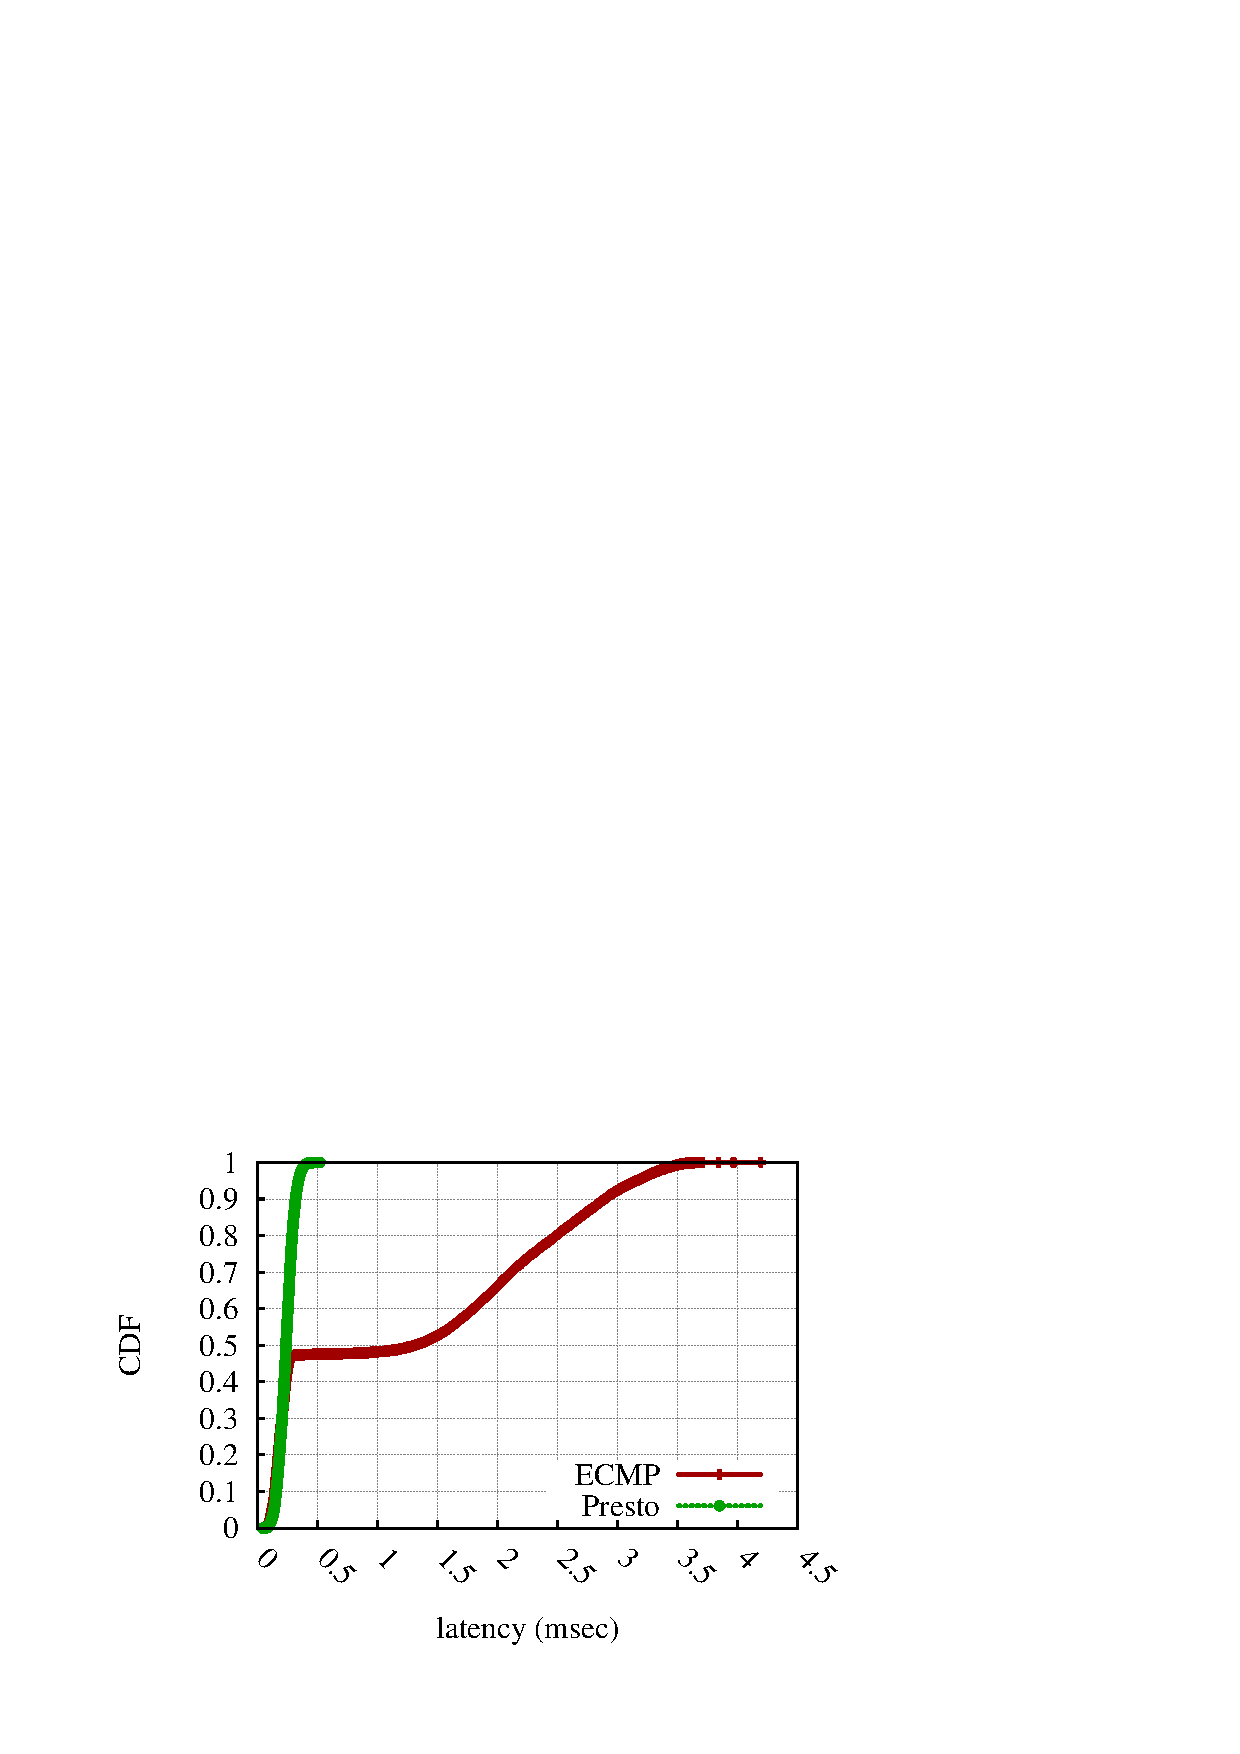
\includegraphics[width=0.45\textwidth]{presto/figures/scalability_test/scalability_compare_latency.pdf}
        \caption{Round trip time comparison in scalability benchmark. 
		%We increase the number of spine switches (i.e., the number of intermediate paths)
                %and set the number of flows (host pairs) equal to the number of available paths. 
		}
        \label{micro_scalability_test_latency}
\end{figure}


\begin{figure}[t]
        \centering
	\centering
        \begin{subfigure}[b]{0.225\textwidth}
                \centering
		\includegraphics[width=\textwidth]{presto/figures/scalability_test/scalability_compare_loss.pdf}
		\caption{}
		\label{micro_scalability_test_loss}
        \end{subfigure}
        \begin{subfigure}[b]{0.225\textwidth}
  		\includegraphics[width=\textwidth]{presto/figures/scalability_test/scalability_compare_fairness.pdf}
        	\caption{}
        	\label{micro_scalability_test_fairness}
	\end{subfigure}
	\caption{(a) Loss rate and (b) Fairness index comparison in scalability benchmark.}
\end{figure}

\tightparagraph{Presto Scales to Multiple Paths}
We analyze Presto's ability to scale in the number of paths by
setting the number of flows (host pairs) equal to the number of available paths in the topology shown in 
Figure~\ref{micro_scalability_topology}. The number of paths is varied from 2 to 8, and 
Presto always load-balances over all available paths.
Figure~\ref{micro_scalability_test_tput} shows Presto's throughput closely tracks Optimal. 
ECMP (and MPTCP) suffer from lower throughput when flows (or subflows) are
hashed to the same path. Hashing on the same path leads to congestion and thus increased latency, as shown in Figure~\ref{micro_scalability_test_latency}.
Because this topology is non-blocking and Presto load-balances in a near optimal fashion, Presto's latency
is near Optimal. Packet drop rates are presented in Figure~\ref{micro_scalability_test_loss} and show
Presto and Optimal have no loss. MPTCP has higher loss because of its bursty nature~\cite{conga}
and its aggression in the face of loss: when a single loss occurs, only
one subflow reduces its rate. The other schemes are more conservative because a single loss reduces the rate of the whole flow.
Finally, Figure~\ref{micro_scalability_test_fairness} shows Presto, Optimal and MPTCP
achieve almost perfect fairness.
%The underlying reason is that MPTCP makes traffic more bursty~\cite{conga}.


%%%congestion test figures %%%%
\begin{figure}[t]
        \centering
  \includegraphics[width=0.45\textwidth]{presto/figures/congestion_test/congestion_compare_tput_witherrbar.pdf}
        \caption{Throughput comparison in oversubscription benchmark.}
        \label{micro_congestion_test_tput}
\end{figure}


\begin{figure}[t]
        \centering
  \includegraphics[width=0.45\textwidth]{presto/figures/congestion_test/congestion_compare_latency.pdf}
        \caption{Round trip time comparison in oversubscription benchmark.
		}
        \label{micro_congestion_test_latency}
\end{figure}



\begin{figure}[t]
        \centering
	\centering
        \begin{subfigure}[b]{0.225\textwidth}
                \centering
		\includegraphics[width=\textwidth]{presto/figures/congestion_test/congestion_compare_loss.pdf}
		\caption{}
		\label{micro_congestion_test_loss}
	\end{subfigure}
	\begin{subfigure}[b]{0.225\textwidth}
		\centering
  		\includegraphics[width=\textwidth]{presto/figures/congestion_test/congestion_compare_fairness.pdf}
		\caption{}
        \label{micro_congestion_test_fairness}
	\end{subfigure}
	\caption{(a) Loss rate and (b) Fairness index comparison in oversubscription benchmark.}
\end{figure}

\tightparagraph{Presto Handles Congestion Gracefully}
Presto's ability to handle congestion is analyzed by fixing 
the number of spine and leaf switches to 2 and varying
the number of flows (host pairs) from 2 to 8, as shown
in Figure~\ref{micro_congestion_topology}. 
Each flow sends as much as possible, which leads to the network
being oversubscribed by a ratio of 1 (two flows) to 4 (eight flows).
Figure~\ref{micro_congestion_test_tput} shows all schemes track Optimal in highly
oversubscribed environments. ECMP
does poorly under moderate congestion because the limited number of flows can be hashed to the same path.
Presto does no worse in terms of latency (Figure~\ref{micro_congestion_test_latency}) and loss (Figure~\ref{micro_congestion_test_loss}).
The long tail latency for MPTCP is caused by its higher loss rates.
Both Presto and MPTCP have greatly improved fairness compared with ECMP (Figure~\ref{micro_congestion_test_fairness}).

\begin{figure}[!t]
        \centering
  \includegraphics[width=0.45\textwidth]{presto/figures/flowlets/flowlet_switching/flowlet_presto_compare_sockperf.pdf}
        \caption{Round trip time comparison of flowlet switching and Presto in Stride workload. 
		The throughputs of Flowlet switching with 100 $\mu\text{s}$ gap, 500 $\mu\text{s}$ gap and Presto 
		are 4.3 Gbps, 7.6 Gbps and 9.3 Gbps respectively. }
        \label{micro_flowlet_rtt_compare}
\end{figure}


\tightparagraph{Comparison to Flowlet Switching}
We first implemented a flowlet load-balancing scheme in OVS that detects
inactivity gaps and then schedules flowlets over disjoint paths in a round robin fashion.
%(Presto does this over flowcells instead of flowlets).
The receiver for flowlets uses official GRO.
Our flowlet scheme is not a direct reflection of CONGA because (i) it is not 
congestion-aware and (ii) the flowlets are determined in the software edge
instead of the networking hardware.
Presto is compared to 500 $\mu$s and 100 $\mu$s inactivity timers in
the stride workload on the 2-tier Clos network (Figure~\ref{macro_evaluation_topology}).
The throughput of the schemes are 9.3 Gbps (Presto), 7.6 Gbps (500 $\mu$s), and 4.3 Gbps (100 $\mu$s).
%Switching flowlets on very small timescales, such as 100$\mu$s, provides opportunities to create many flowlets.
%The largest flowlet is only 0.20\% (XX) of the total network traffic, which corresponds to about 5-9 MB in our runs.
%And while small flowlets create an even distribution
%of traffic over the network, significant strain is put on the TCP connection due to packet reordering. 
Analysis of the 100 $\mu$s
network traces show 13\%-29\% packets in the connection are reordered, which means 100 $\mu$s is not enough
time to allow packets to arrive in-order at the destination and thus throughput is severely impacted. Switching flowlets with 500 $\mu$s prevents
most reordering (only 0.03\%-0.5\% packets are reordered), but creates very large flowlets (see Figure~\ref{micro_flowlet_size}). This means
flowlets can still suffer from collisions, which can hurt throughput (note: while not shown here, 500 $\mu$s outperforms ECMP by over 40\%).
Figure~\ref{micro_flowlet_rtt_compare} shows the
latencies. Flowlet 100 $\mu$s has low throughput and hence lower latencies. However, since
its load balancing isn't perfect, it can still cause increased congestion in the tail. Flowlet 500 $\mu$s
also has larger tail latencies because of more pronounced flowlet collisions. As compared to the flowlet
schemes, Presto decreases 99.9$^{th}$ percentile latency by 2x-3.6x.
%Presto, by enforcing small flowlet sizes and explicitly accounting for reordering on the receiver, can obtain near
%line rate throughput with minimal tail latencies. 



%%%%presto 2 mods (ecmp and shaodw MAC) compare
\begin{figure}[!t]
        \centering
  \includegraphics[width=0.45\textwidth]{presto/figures/presto_compare_2modes/presto_compare_2mods.pdf}
        \caption{Round trip time comparison between Presto + shadow MAC and Presto + ECMP.
		%Compare Presto 2 modes' (Presto over ECMP and Presto over Shadow MAC) performance.
                %Simple 2-tier Clos network with 4 senders and 4 receivers, 4 paths between any host pair.
                %10 seconds per run, 20 runs. Use {\tt nuttcp} to measure throughput. Use {\tt sockperf}
                %to measure latency (RTT).
                %In Presto+ECMP, the average throughput is 7.9 (8.7 if trade latency for tput)
                %Gbps while in Presto+Shadow MAC, the
                %average throughput is 9.3Gbps 
		}
        \label{micro_presto_2mods}
\end{figure}

\tightparagraph{Comparison to Local, Per-Hop Load Balancing}
Presto sends flowcells in a round robin fashion over pre-configured end-to-end paths. An alternative is to
have ECMP hash on flowcell ID and thus provide per-hop load balancing. 
%One way to implement Presto + ECMP is to let vSwitch copy real TCP source port into a pre-allocated TCP option field 
%(\todo{this requires TCP stack allocates the new TCP option before sending to vSwitch}) and 
%encode chunk ID into TCP source port field. Because chunk ID is incremental, ECMP randomly maps chunks into multiple paths. 
We compare Presto + shadow MAC with Presto + ECMP using a stride workload on our testbed. 
Presto + shadow MAC's average throughput is 9.3 Gbps while Presto + ECMP's is 8.9 Gbps.
The round trip time CDF is shown in Figure~\ref{micro_presto_2mods}. 
Presto + shadow MAC gives better latency performance compared with Presto + ECMP. 
The performance difference comes from the fact that Presto + shadow MAC provides 
better fine-grained flowcell load balancing because 
randomization in per-hop multipathing can lead to corner cases where
a large fraction of flowcells get sent to the same link over a small timescale by multiple flows. This transient congestion
can lead to increased buffer occupancy and higher delays.

\section{Evaluation}
\label{sec:eval}

%~\todo{needs to go through the text and make sure they are consistent with the figures!!!}
In this section, we analyze the performance of Presto for (i) synthetic workloads, (ii)
trace-driven workloads, (iii) workloads containing north-south cross traffic, and (iv) failures.
All tests are run on the topology in Figure~\ref{macro_evaluation_topology}.
\begin{figure}[!t]
        \centering
  \includegraphics[width=0.45\textwidth]{./figures/macro/stride/macro_compare_tput_witherrbar.pdf}
        \caption{Elephant flow's throughputs of ECMP, MPTCP, Presto and Optimal in Shuffle, Random, Stride and Random Bijection workloads.}
        \label{macro_evaluation_tput}
\end{figure}



\begin{figure*}[!t]
        \centering
	\begin{subfigure}[b]{0.3\textwidth}
                \centering
  		\includegraphics[width=\textwidth]{./figures/macro/stride/macro_compare_fct_stride_mice.pdf}
        	\caption{Stride}
        	\label{macro_evaluation_fct_stride}
	\end{subfigure}
	\begin{subfigure}[b]{0.3\textwidth}
                \centering
		\includegraphics[width=\textwidth]{./figures/macro/bijection/macro_compare_fct_bijection_mice.pdf}
        	\caption{Random Bijection}
        	\label{macro_evaluation_fct_bijection}
	\end{subfigure}
        %\begin{subfigure}[b]{0.225\textwidth}
        %        \centering
	%	\includegraphics[width=\textwidth]{./figures/macro/random/macro_compare_fct_random_mice.pdf}
        %	\caption{Random}
        %	\label{macro_evaluation_fct_random}
	%\end{subfigure}
        \begin{subfigure}[b]{0.3\textwidth}
                \centering
		\includegraphics[width=\textwidth]{./figures/macro/shuffle/macro_compare_fct_shuffle_mice.pdf}
        	\caption{Shuffle}
        	\label{macro_evaluation_fct_shuffle}
	\end{subfigure}
	\caption{Mice FCT of ECMP, MPTCP, Presto and Optimal in stride, random bijection, and shuffle workloads.}
	\label{macro_evaluation_fct}
\end{figure*}

\tightparagraph{Synthetic Workloads}
Figure~\ref{macro_evaluation_tput} 
shows the average throughputs of elephant flows in the shuffle, random, stride and random bijection workloads.
Presto's throughput is within 1-4\% of Optimal over all workloads.
For the shuffle workload, ECMP, MPTCP, Presto and Optimal show similar results 
because the throughput is mainly bottlenecked at the receiver. 
%due to several servers sending to the same receiver.
In the non-shuffle workloads, Presto improves upon ECMP by 38-72\% and improves
upon MPTCP by 17-28\%.
%Compared with ECMP, 
%Presto improves throughput by 71\% (stride), 72\% (random bijection) and 38\% (random).
%Presto also outperforms MPTCP with throughput improvements of 23\% (stride), 28\% (random bijection) and 
%17\% (random).
%In all the workloads, Presto's throughput outperforms MPTCP.

Figure~\ref{macro_evaluation_fct} shows the mice flow completion time (FCT) in
the workloads. 
The stride and random bijection workloads are non-blocking, and hence the latency of Presto
closely tracks Optimal: the 99.9$^{th}$ percentile FCT for Presto is within 350 $\mu$s for these workloads.
MPTCP and ECMP suffer from congestion, and therefore the tail FCT is much worse than Presto: ECMP's 99.9$^{th}$ percentile
FCT is over 7.5x worse ($\sim$11ms) and MPTCP experiences timeout (because of higher loss
rates and the fact that small sub-flow window sizes from small flows can increase the chances of timeout~\cite{dc-mptcp}).\footnote{We used the Linux default (200ms) and trimmed graphs for clarity}
The difference in the random and shuffle workloads is less pronounced (we omit random due to space constraints).
In these workloads elephant flows can collide on the last hop output port,
and therefore mice FCT is mainly determined by queuing latency. In shuffle, the 99.9$^{th}$ percentile FCT for ECMP, Presto and Optimal
are all within 10\% (MPTCP again experiences TCP timeout) and in random, the 99.9$^{th}$ percentile FCT of Presto is within 25\% of Optimal while ECMP's 
is 32\% worse than Presto.


%%the following are combined into one figure
\iffalse
\begin{figure}[!t]
        \centering
  \includegraphics[width=0.45\textwidth]{./figures/macro/bijection/macro_compare_fct_bijection_mice.pdf}
        \caption{Macro evaluation - flow completiom time in Random Bijection workload}
        \label{macro_evaluation_fct_bijection}
\end{figure}

\begin{figure}[!t]
        \centering
  \includegraphics[width=0.45\textwidth]{./figures/macro/random/macro_compare_fct_random_mice.pdf}
        \caption{Macro evaluation - flow completiom time in Random workload}
        \label{macro_evaluation_fct_random}
\end{figure}


\begin{figure}[!t]
        \centering
  \includegraphics[width=0.45\textwidth]{./figures/macro/shuffle/macro_compare_fct_shuffle_mice.pdf}
        \caption{Macro evaluation - flow completiom time in Shuffle workload}
        \label{macro_evaluation_fct_shuffle}
\end{figure}

\fi

\iffalse
\begin{table}[!htb]
\begin{center}
\begin{tabular}{ |c|c|c|c|c| } 
 \hline
 Shuffle & ECMP & MPTCP & Presto & Optimal \\
 \hline 
 Median & 401 & 874 & 387 & 369  \\ 
 90\%   & 1037 & 2664 & 726 & 712 \\
 99\%   & 3373 & 21600  & 2447 & 2446 \\ 
 99.9\% & 12830 & 206ms & 12480 & 11714 \\
 %99.99\% & 204.1ms & - & 204.1ms & 203.6ms \\
 \hline

\end{tabular}
\caption{Macro evaluation - A close look of flow completiom time in Shuffle workload}
        \label{macro_evaluation_fct_shuffle_closelook}
\end{center}
\end{table}

\begin{table}[!htb]
\begin{center}
\begin{tabular}{ |c|c|c|c|c| }
 \hline
 Random & ECMP & MPTCP & Presto & Optimal \\
 \hline
 Median & 1008 & 780 & 648 & 595  \\
 90\%   & 3815 & 1918 & 2850 & 2297 \\
 99\%   & 7852 & 3380  & 6900 & 4936 \\
 99.9\% & 11784 & 202ms & 9372 & 7127 \\
% 99.99\% & 11677 & - & 16591 & 200ms \\
 \hline

\end{tabular}
\caption{Macro evaluation - A close look of flow completiom time in Random workload}
        \label{macro_evaluation_fct_random_closelook}
\end{center}
\end{table}

\fi

%%% trace-driven workload, MSR, scaling factor =10
\begin{table}[!tb]
\begin{center}
\begin{tabular}{ |c|c|c|c| }
 \hline
 Percentile & ECMP & Optimal &Presto \\
 \hline
 50\%   & $1.0$ & $-12\%$ & $-9\%$   \\
 90\%   & $1.0$ & $-34\%$ & $-32\%$  \\
 99\%   & $1.0$ & $-63\%$  & $-56\%$ \\
 99.9\% & $1.0$ & $-61\%$ & $-60\%$  \\
 \hline

\end{tabular}
\caption{Mice ($<$100KB) FCT in trace-driven workload~\cite{kandula2009nature}. Negative numbers imply shorter FCT.}
        \label{macro_evaluation_MSR_trace_driven}
\end{center}
\end{table}

\tightparagraph{Trace-driven Workload}
We evaluate Presto using a trace-driven workload based on traffic patterns measured in~\cite{kandula2009nature}. 
Each server establishes a long-lived TCP connection 
with every other server in the testbed. 
Then each server continuously samples flow sizes and inter-arrival times and each time sends to a random receiver
that is not in the same rack.
%Since 99\% of flows are less than 4MB in the distribution, 
We scale the flow size distribution by a factor of 10 to emulate a heavier workload. 
Mice flows are defined as flows that are less than 100 KB in size, and elephant flows are defined as flows
that are greater than 1 MB. The mice FCT, normalized to ECMP, 
is shown in Table~\ref{macro_evaluation_MSR_trace_driven}. 
Compared with ECMP, Presto has similar performance at the 50$^{th}$ percentile but reduces the 99$^{th}$ and 99.9$^{th}$ percentile FCT by 56\% and 60\%, respectively. 
Note MPTCP is omitted because its performance was quite unstable in workloads
featuring a large number of small flows.
The average throughput (not shown) for Presto tracks Optimal (within 2\%), and improves upon ECMP by over 10\%.


\begin{table}[!htb]
\begin{center}
\begin{tabular}{ |c|c|c|c|c| }
 \hline
% Percentile & 50\% & 90\% & 99\% & 99.9\% \\
% \hline
% ECMP & 1.0 & 1.0 & 1.0 & 1.0  \\
% N-block   & 66\% & 17\% & 11\% & 9\% \\
% Presto    & 80\% & 21\% & 14\% & 10\% \\
% MPTCP     & 88\% & 27\% & 27\% & TIMEOUT \\

 Percentile & ECMP & Optimal & Presto & MPTCP \\
 \hline
 50\%       & 1.0 & $-34$\%     & $-20$\%   & $-12$\% \\
 90\%       & 1.0 & $-83$\%     & $-79$\%   & $-73$\% \\
 99\%       & 1.0 & $-89$\%     & $-86$\%   & $-73$\% \\
 99.9\%     & 1.0 & $-91$\%      & $-87$\%   & TIMEOUT \\

 \hline
\end{tabular}
\caption{FCT comparison (normalized to ECMP) with ECMP load balanced north-south traffic.}
	\label{macro_evaluation_north_south_traffic}
\end{center}
\end{table}


\tightparagraph{Impact of North-South Cross Traffic}
Presto load balances on "east-west" traffic in the datacenter, \ie{}, traffic
originating and ending at servers in the datacenter. 
In a real datacenter environment "north-south" traffic (\ie{}, traffic with an endpoint outside the datacenter)
must also be considered. 
%Ideally, north-south traffic should be load balanced by ECMP because of 
%reordering concerns at the end user. 
%However, east-west traffic typically dominates (75\% according to~\cite{east-west}). 
To study the impact of north-south traffic on Presto, we attach an additional server to 
each spine switch in our testbed to emulate remote users. 
The 16 servers establish a long-lived TCP connection with each remote user. 
Next, each server starts a flow to a random remote user every 1 millisecond. This emulates  
the behavior of using ECMP to load balance north-south traffic.
The flow sizes for north-south traffic are based on the distribution measurement in~\cite{he2013next}. 
The throughput to remote users is limited to 100Mbps to emulate the limitation of an Internet WAN. 
Along with the north-south flows, 
a stride workload is started to emulate the east-west traffic. 
The east-west mice FCT is shown in Table~\ref{macro_evaluation_north_south_traffic} (normalized to ECMP). 
ECMP, MPTCP, Presto, and Optimal's average throughput is 
5.7, 7.4, 8.2, and 8.9Gbps respectively. 
The experiment shows Presto can gracefully co-exist with north-south cross traffic
in the datacenter.


%%%failure handling experiments

\begin{figure}[t]
        \centering
  \includegraphics[width=0.45\textwidth]{./figures/failure_handling/failover_compare_tput_witherrbar.pdf}
        \caption{Presto's throughput in symmetry, fast failover and weighted multipathing stages for different workloads.}
        \label{failover_compare_tput}
\end{figure}

\begin{figure}[t]
        \centering
  \includegraphics[width=0.45\textwidth]{./figures/failure_handling/failover_compare_sockperf_bijection_mice.pdf}
        \caption{Presto's RTT in symmetry, fast failover and weighted multipathing stages in  random bijection workload.}
        \label{failover_compare_sockperf_bijection}
\end{figure}

\tightparagraph{Impact of Link Failure}
Finally, we study the impact of link failure.
Figure~\ref{failover_compare_tput} compares the throughputs of
Presto when %under different stages of loss recovery when 
the link between spine switch S1 and leaf switch L1 goes down.
Three stages are defined: symmetry (the link is up), failover (hardware fast-failover moves traffic from S1 to S2), and weighted (the controller
learns of the failure and prunes the tree with the bad link).
Despite the asymmetry in the topology, Presto still achieves reasonable average throughput at 
each stage.
Figure~\ref{failover_compare_sockperf_bijection} shows the round trip time of
each stage in a random bijection workload. 
Workload L1->L4 is when each node connected to L1 sends to one node in L4 (L4->L1 is the opposite).
Due to the fact that the network is no longer non-blocking after the link failure,
failover and weighted multipathing stages have larger round trip time.



\iffalse
\begin{enumerate}
\item Clos-network, macro. ECMP, MPTCP, Presto and Optimal.
\begin{enumerate}
	\item Workloads: Take from Planck and Hedera. Can do MSR trace-based.
	\item Throughput, fairness, latency (maybe loss). Link utilization?
\end{enumerate}

\item Fat tree, macro. ECMP, MPTCP, Presto and Optimal.
\begin{enumerate}
        \item Workloads: Take from Planck and Hedera. Can do MSR trace-based.
        \item Throughput, fairness, latency (maybe loss). Link utilization?
\end{enumerate}


\item Vary flow sizes. Idea is that we can work on very small elephants.

\item Failure: backbone switch fails, aggregate switch fails, ToR switch fails, link fails, ...

\item CONGA uses incast, should we check?

\item Maybe this belongs in micro: ECMP vs shadowMAC for multipathing.

\end{enumerate}
\fi

%\section{Related Work}
\label{sec:related}
We summarize the related work into three categories: datacenter traffic load balancing, reducing tail latency and handling packet reordering.

{\bf Load Balancing in Datacenters} 
%Load balancing in datacenter networks has been the focus of several studies.
MPTCP~\cite{mptcp,dc-mptcp} is a transport protocol that uses subflows to 
transmit over multiple paths.
CONGA~\cite{conga} and Juniper VCF~\cite{juniper-vcf} both employ congestion-aware flowlet switching~\cite{flowlet} on
specialized switch chipsets to load balance the network.
RPS~\cite{packetspray} and DRB~\cite{drb} evaluate per-packet load balancing on symmetric 1 Gbps networks
at the switch and end-host, respectively.
The CPU load and feasibility of end-host-based per-packet load balancing for 10+ Gbps networks remains open.
%Per-packet load balancing can incur significant end-host overhead for DRB
%if not resorting to jumbo frames.
%Packet reordering problem is not well considered in both RPS and DRB.
%RPS and DRB may perform worse than ECMP in case of topology asymmetry.
Hedera~\cite{hedera}, MicroTE~\cite{microte} and Planck~\cite{planck} use centralized traffic engineering to
reroute traffic based on network conditions.
FlowBender~\cite{flowbender} reroutes flows when congestion is detected by end-hosts and 
Fastpass~\cite{fastpass} employs a centralized arbiter to schedule path selection for each packet.
As compared to these schemes, Presto is the only one that proactively load-balances at line rate for fast networks
in a near uniform fashion without requiring additional infrastructure or changes
to network hardware or transport layers. Furthermore, to the best of our knowledge, Presto is
the first work to explore the interactions of fine-grained load balancing with built-in
segment offload capabilities used in fast networks.
%\textcolor{blue}{~\cite{eden} also advocates to implement network functions such as load balancing 
%at datacenter end hosts.}

{\bf Reducing Tail Latency}
%Detail~\cite{detail} summarizes the causes of long tails of flow completion time---
%1)packet loss and retransmissions,
%2)absence of flow prioritization and 3)uneven load balancing.
%Reducing tail latencies of small mice flows has also been actively studied.
DeTail~\cite{detail} is a cross-layer network stack designed to reduce the tail of flow completion times.
%link layer uses port buffer occupancy to construct lossless fabric,
%network layer performs per-packet adaptive load balancing based on port buffer occupancy,
%transport layer relies upon congestion notifications
%derived from port buffer occupancies,
%finally Detail lets application layer specify flow priorities to
%avoid head-of-line blocking of elephant flows for mice time-sensitive flows.
%Detail modified many layers (including the switch) and is hard to deploy using
%current hardware and network stack.
DCTCP~\cite{dctcp} is a transport protocol that uses the portion of marked packets 
by ECN to adaptively adjust sender's TCP's congestion window to reduce switch buffer occupancy.
%Thus, DCTCP can reduce switch buffer occupancy and reduce flow completion time.
HULL~\cite{hull} uses Phantom Queues and congestion notifications to cap link utilization and prevent congestion.
%HULL uses packet pacing to combat with traffic burstiness in order to leave "bandwidth headroom".
In contrast, Presto is a load balancing system that naturally improves 
the tail latencies of mice flows by uniformly spreading traffic in 
fine-grained units.
%We share the overall goal of reducing mice tail latencies, but instead explore how
%fine-grained load balancing can provide a solution.
QJUMP~\cite{qjump} utilizes priority levels to 
allow latency-sensitive flows to "jump-the-queue" over low priority flows.
PIAS~\cite{pias} uses priority queues to mimic the Shortest Job First principle to reduce FCTs.
%solve the network interference problem caused by elephant and mice flows 
%for datacenter networks. High priority packets are rate-limited 
%at the end-host and can "jump-the-queue" over packets with 
%lower priorities. PIAS~\cite{pias} mimics the Shortest Job First (SJF) 
%principle to reduce flow completion times. It gradually decreases 
%the priority level assigned to a flow based on its flow size.
%Presto is complementary and could be applied on each priority level.
%DIBS~\cite{dibs} detours packets of a congested switch port to a randomly 
%picking neighboring switch to reduce packet drops.
Last, a blog post by Casado and Pettit~\cite{vmware} summarized
four potential ways to deal with elephants and mice, with one advocating
to turn elephants into mice at the edge. 
We share the same motivation and high-level
idea and design
a complete system that addresses many practical challenges of using
such an approach.

%%%%%the follwoing may not be used
\iffalse
WCMP~\cite{wcmp} reduces the number of TCAM/SRAM entries to implement 
Weighted Cost Multipathing for asymmetry network topologies 
by approximating the path weights. 
Different from WCMP, Presto assigns path weights in openvswitch (i.e., host memory), 
thus Presto is not limited by TCAM resource. 
Similar to WCMP, Presto can perform near-optimal traffic striping in asymmetry topologies because
the weights are determined by a global view of the network.

VL2~\cite{vl2} uses flat addressing to allow service instances to be placed anywhere in the network. 
It leverages a shim-layer on end-hosts to perform IP-in-IP encapsulation to 
decouple topological address from flat application address.
Portland~\cite{portland} uses positional pseudo MAC address to decouple forwarding address from service address. 
VXLAN~\cite{vxlan} and NVGRE~\cite{nvgre} use tunneling mechanism (virtualized L2 networks over L3 network) to 
enable applications to be deployed and migrated between any server regardless of physical server location. 
Presto achieves Ethernet L2 semantics via employing shadow MAC~\cite{shadow-mac}, 
where shadow MAC serves as forwarding address while providing the opportunity to do load balancing.
\fi

{\bf Handling Packet Reordering}
%Many schemes have tried to mitigate the impact of reordering.
TCP performs poorly in the face of reordering, and thus several studies
design a more robust alternative~\cite{rr-tcp,blanton2002making,tcp-pr}.
Presto takes the position that reordering should be handled below TCP in the existing 
receive offload logic.
In the lower portion of the networking stack, SRPIC~\cite{wu2009sorting} sorts reordered packets 
in the driver after each interrupt coalescing event. While this approach can help
mitigate the impact of reordering, it does not sort packets across interrupts, have a 
direct impact on segment sizes, or distinguish between loss and reordering. 
%SRPIC is 
%complementary to our approach because their actions are taken in the driver, before packets
%are pushed to GRO.
%RR-TCP~\cite{rr-tcp} proposed to extend TCP sender to detect and recover from false fast retransmits using DSACK information. 
%As we show, fixing TCP itself cannot solve all the problems incurred by packet reordering.
%\eric{i have some LRO references in the patent slides that we need to make sure are cited somewhere} 
%Instead, Presto's chunking scheme leverages the fact that all the packets going through the same path are in order and has two nice properties:
%1)Presto uses chunkid to make the task of distinguishing packet loss from temporary packet reordering much simpler. 
%2)Presto only needs to make sure the chunks are in order instead of packets, thus reducing per-packet processing overhead.

%\section{Discussion}
\label{discuss}

\tightparagraph{UDP traffic} How to handle. 
Mention VxLAN traffic too.
\keqiang{and IPsec}

\tightparagraph{No vSwitch} 
\keqiang{title should be hypervisor-bypass?}
Use middleboxes (for DB server).
Use NIC (for SR-IOV).
Hypervisor bypass (e.g., SR-IOV), where TCP traffic is sent to the NIC directly without 
going through hypervisor. First, as noted by~\cite{shieh2011sharing}, ``loss of the security and 
manageability features provided by the software virtual switch has limited 
the deployment of direct I/O NICs in public clouds''. Second, based on techniques like Intel 
DPDK~\cite{intel-dpdk} and ``smart NICs''~\cite{cavium-nic,netronome-nic}, we believe that low latency 
congestion control enforcement schemes like \acdc{} can also be 
employed for hypervisor bypass use cases.
We need to worry about legacy systems and non-VM systems. For instance, a database or storage device that may not have OVS installed on it.
We need to talk about either a middlebox or that this percentage of traffic is low? Or implement in NIC (especially one with OVS offload?).

\tightparagraph{North-South traffic.}
Transport enforcement should be only be done for east west traffic, so if the tenant tuned their stack's
congestion control algorithm for wide-area networks, their north sourth traffic is not affected and their 
congestion control scheme can still achieve good performance.

\keqiang{todos: some figures do not read well on printed paper}
\keqiang{todos: sometimes, when we refer a section, we say ``Section X'', sometimes, we use the 
dollar sign, we should unify them}

%
%Byzantine VM.
%
%Other names: ACDCTCP, LiquidSwitch, LiquidEdge
%
%In CPU overhead measurement, we need to 
%mention ovs add 1 widecard rule. That means we isolated the overhead of 
%OVS itself when it has many flows in its flow table (probably it does not matter
%at the end of the day, because we measured the CPU usage of the whole system).
%
%People may say window-based congestion control is burty. TIMELY operates 
%on TCP segments in order to reduce CPU overhead. Therefore, TIMELY is also
%busty. In TIMELY, they mentioned they can leverage a hybrid scheme, that is
%using software to control large segments and use hardware rate limiter to
%reduce burstyness.
%
%Create loss and check how DCTCP and our scheme treates packet losses (revisit it after we finish incast 
%and macrobenchmarks).
%
%One more microbenchmark on the Dumbbell topology: different servers have different transport, so the
%throughput fairness among different transports (e.g., start cubic, start New Reno, start dctcp).
%
%A point that is missing in DCTCP and NSDI paper is that they did not mention how the switch should be
%configured to handle non-TCP traffic. Note non-TCP traffic such as DNS (UDP 53) and ARP, ICMP etc
%are also important. We found that if we did not specify how the switch handle the non-TCP traffic,
%then this kind of non-TCP traffic can be easily dropped by the switch. We found ARP traffic is dropped
%by the switch such that DCTCP flows stall. Hence, we think it is better to put non-TCP traffic
%into a different queue when we apply WRED/ECN on the switches.
%
%This work offers low latency for ``hetergeneous networks" where different entities can 
%run different kinds of
%transport congestion control schemes. A few examples of such hetergeneous networks: public 
%datacenters where tenants can set up their own VMs (e.g., AWS), or tenants can rent their bare metal
%machines (e.g., SoftLayer), or certain groups (even within a single organization) 
%have to use traditional transports due to compatibility of legacy applications (NSDI's Judd said this), or
%incremental deployment is undergoing. 
%To ensure a pure low latency datacenter network, a universal transport enforcement scheme is required. 
%Two challenges to implement such a transport enforcement scheme are scalability and low overhead. 
%The transport enformancement scheme proposed here meet the two metrics (as shown in our experiments) while
%providing nice network performance (throughput, latency and packet drop rate). This scheme is 
%compatible with any kind of TCP stack. Finally, the scheme we propose solves the co-existence issue of 
%ECT (ECN Capable Transport) and non-ECT, which is a critical deployment hurdle for DCTCP-like transports.
%
%Macrobenchmark plan: 18 hosts, 6 switches, ECMP configured. The network oversubscription ratio is 2:1.
%Run all-to-all traffic for a long time (e.g., 1 hours). Show total throughput and TCP RTT and packet drop 
%rate.
%
%QoS can be implemented too?
%
%
%
%When we try to launch an instance in EC2: ``An AMI is a template that contains the software 
%configuration (operating system, application server, and applications) required to launch your instance. 
%You can select an AMI provided by AWS, our user community, or the AWS Marketplace; 
%or you can select one of your own AMIs''. Default is CUBIC for most Linux images, Window Servers can
%have NewReno, Compound TCP (CTCP)~\cite{tan2006compound} and DCTCP. 
%Users can tweak congestion control algorithms to optimize network performance for their target scenarios. 
%
%Section talking about how to implement other CC schemes: TIMELY, PERC, Vegas, etc.
%
%EJR: VXLAN, UDP, TCP stack statistics for Cloud?
%
%ECT and non-ECT: througput unfairness, long RTT, connection establishment..
%
%
%EyeQ, Seawall, NetShare, Silo, SecondNet, Oktopus etc. Our work did not provide bandwidth allocation property. 
%This work focused on reducing in-network queuing latency caused by VM TCP stacks. 
%We show how this goal can be done using a simple and elegant solution.
%Yes, if an VM opens more connections than another, that VM gains more bandwidth. 
%But, there are proposals which try to provide proper bandwidth allocation when multiple end-points compete 
%at the sender side or receiver side. Those works and this work are complementary. 
%To the best of our knowledge, today's cloud providers have not provide strong bandwidth guarantees 
%(for example, AWS only roughly classify VMs instances' network performance into 
%``low to moderate", ``moderate", ``high" and ``10 Gigabit"categories).
%
%talk about containers?

\section{Summary}
\label{sec:conclusion}
In this paper, we present Presto: a near uniform sub-flow distributed load balancing scheme
that can near optimally load balance the network at fast networking speeds.
Our scheme makes a few changes to the hypervisor soft-edge (vSwitch and GRO)
and does not require any modifications to the transport layer or network hardware, making
the bar for deployment lower. 
%Working at fast networking speeds poses many challenges,
Presto is explicitly designed to load balance the network at fine granularities
and deal with reordering without imposing much overhead on hosts. Presto is flexible and can also
deal with failures and asymmetry. Finally, we show the performance of Presto can closely track
that of an optimal non-blocking switch, meaning elephant throughputs remain high while the tail
latencies of mice flow completion times do not grow due to congestion.



\chapter{Virtual Congestion Control Enforcement for Datacenter Networks}
\label{thesis:chapter:acdctcp}


\section{Introduction}
\label{intro}

Multi-tenant datacenters are a crucial component of today's computing ecosystem. Large providers, such as Amazon, Microsoft, IBM, Google and Rackspace, support
a diverse set of customers, applications and systems through their public cloud offerings. These offerings are successful in 
part because they provide efficient performance to a wide-class of applications running on a diverse set of platforms. Virtual
Machines (VMs) play a key role in supporting this diversity by allowing customers to run applications in a wide variety of 
operating systems and configurations.

And while the flexibility of VMs allows customers to easily move a vast array of applications into the cloud, that same flexibility inhibits the 
amount of control a cloud provider yields over VM behavior. For example, a cloud provider may be able to provide virtual networks or enforce rate limiting
on a tenant VM, but it cannot control the VM's TCP/IP stack. As the TCP/IP stack considerably impacts overall network performance, it 
is unfortunate that cloud providers cannot exert a fine-grained level of control over one of the most important components in the networking stack.

Without control over the VM TCP/IP stack, datacenter networks remain at the mercy of inefficient, out-dated or misconfigured TCP/IP stacks.
TCP behavior, specifically congestion control, has been widely studied and many issues have come to light when it is not optimized. For example,
network congestion caused by non-optimzed stacks can lead to loss, increased latency and reduced throughput. 
%As revenue increasingly is tied to 
%strict latency and bandwidth requirements from workloads such as big data analytics and search~\cite{alizadeh2011data,dean2013tail}, public cloud providers must ensure their
%network fabrics can provide tight service-level agreements and deadlines required by customer applications.

Thankfully, recent advances optimizing TCP stacks for datacenters have shown high throughput and low latency can be 
achieved through novel TCP congestion control algorithms. Works such as DCTCP~\cite{alizadeh2011data} and TIMELY~\cite{mittal2015timely} provide high
bandwidth and low latency by ensuring network queues in switches do not fill up. And while these stacks are deployed in many of today's 
private datacenters~\cite{singh2015jupiter,judd2015nsdi}, ensuring a vast majority of VMs within a public datacenter will update their TCP stacks
to a new technology is a daunting, if not impossible, task.

In this chapter, we explore how operators can regain authority over TCP congestion control, regardless of the TCP stack
running in a VM. Our aim is to allow a cloud provider to utilize advanced TCP stacks, such as DCTCP, without having
control over the VM or requiring changes in network hardware. We propose implementing congestion control in the virtual switch
(vSwitch) running on each server. Implementing congestion control within a vSwitch has several advantages. 
First, vSwitches naturally fit into datacenter network virtualization architectures and are widely
deployed~\cite{Pfaff2015ovs}. Second, vSwitches can easily monitor and modify traffic passing through them. 
Today vSwitch technology is mature and robust, allowing for a fast, scalable,
and highly-available framework for regaining control over the network. 

%Since vSwitch technology supports software-defined networking (say OVS),
%implementing congestion control within the vSwitch can also naturally support advanced congestion control algorithms, such as centralized 
%or proactive schemes (cite). 

Implementing congestion control within the vSwitch has numerous challenges, however. First, in order to ensure adoption rates are high, the 
approach must work without making changes to VMs. 
Hypervisor-based approaches typically rely on rate limiters to limit VM traffic. Rate limiters implemented in
commodity hardware do not scale in the number of flows and software implementations incur high CPU overhead~\cite{radhakrishnan2014senic}. 
Therefore, limiting a VM's TCP flows in a fine-grained, dynamic nature
at scale (10,000's of flows per server~\cite{180302}) with limited computational overhead remains challenging. 
Finally, VM TCP stacks may differ in the features they support (\eg{}, ECN) or the congestion
control algorithm they implement, so a vSwitch congestion control implementation should work under a variety
of conditions. 

This chapter presents Administrator Control over Datacenter TCP (\acdc{} TCP, or simply~\acdc{}), a new technology that implements 
TCP congestion control within a vSwitch to help ensure VM
TCP performance cannot impact the network in an adverse way. At a high-level, the vSwitch monitors all packets for a flow, modifies 
packets to support features not implemented in the VM's TCP stack (\eg{}, ECN) and reconstructs
important TCP parameters for congestion control.~\acdc runs the congestion control logic specified by an administrator and then enforces an intended
congestion window by modifying the receive window (\rwnd{}) on incoming ACKs. A policing
mechanism ensures stacks cannot benefit from ignoring~\rwnd{}.% and can also be used for non-TCP traffic.

Our scheme provides the following benefits. First,~\acdc allows
administrators to enforce a uniform, network-wide congestion control algorithm without changing VMs. When using congestion control algorithms tuned for 
datacenters, this allows for high throughput and low latency. Second,
our system mitigates the impact of varying TCP stacks running on the same fabric. This improves fairness and additionally
solves the ECN co-existence problem identified in production networks~\cite{wu2012tuning,judd2015nsdi}. 
Third, our scheme is easy to implement, computationally lightweight, scalable, and modular so that it is highly complimentary to
performance isolation schemes also designed for virtualized datacenter environments.
The contributions of this chapter are as follows:
\begin{enumerate}
\item The design of a vSwitch-based congestion control mechanism that regains control over the VM's TCP/IP stack
without requiring any changes to the VM or network hardware. 
\item A prototype implementation to show our scheme is effective, scalable, simple to implement, and has~\crs{less than one percentage point} computational overhead in our tests.
%~\todo{We also provide a simple policing scheme to see if tenants are following rules. Add?} 
\item A set of results showing DCTCP configured as the host TCP stack provides nearly identical
performance to when the host TCP stack varies but DCTCP's congestion control is implemented in the vSwitch. We demonstrate how~\acdc{} can improve
throughput, fairness and latency on a shared datacenter fabric.
\end{enumerate}

The outline of this chapter is as follows. Background and motivation are discussed in \cref{background}.~\acdc{}'s design is outlined in \cref{design} and
implementation in \cref{impl}. Results are presented in \cref{results}.


\section{Background and Motivation}
\label{background}
This section first gives a brief background of congestion 
control in the datacenter. Then the motivation for moving congestion
control into the vSwitch is presented. Finally,~\acdc{} is contrasted from a class of related bandwidth
allocation schemes.

\subsection{Datacenter Transport}
\label{ss:dct}
Today's datacenters host applications such as search,
advertising, analytics and retail that require high bandwidth and low latency.
%Large tail latencies often violate the tight timing constraints required by SLAs at scale, and
%have been shown to impact customer experience, result in
%revenue loss~\cite{alizadeh2011data,dean2013tail}, and degrade application performance~\cite{jang2015silo,qjump}.
%Tail latencies are often caused by network congestion.
%The latency of traversing a single switch, NIC and OS network stack is 10--30$\mu$s,
%2.5--32$\mu$s and 15$\mu$s respectively, but a congested port
%on a network switch can consume significant shared memory, causing orders-of-magnitude
%higer latency~\cite{rumble2011s}.
Network congestion, caused by imperfect load balancing~\cite{al2010hedera},
network upgrades or failures, can adversely impact these services. Unfortunately, congestion is
not rare in datacenters. For example, recently Google reported 
congestion-based drops were observed when network utilization approached 25\%~\cite{singh2015jupiter}.
Other studies have shown high variance and substantial increase in the 99.9$^{th}$ percentile latency
for round-trip times in today's datacenters~\cite{wang2010impact,mogul2015inferring}. 
Large tail latencies impact customer experience, result in
revenue loss~\cite{alizadeh2011data,dean2013tail}, and degrade application performance~\cite{jang2015silo,qjump}.
Therefore, significant motivation exists to reduce congestion in datacenter fabrics.

%Studies have shown that while CUBIC can achieve
%high bandwidth, it does so at the cost of aggressively filling up the switch buffers in the network.
TCP's congestion control algorithm is
known to significantly impact network performance.
As a result, datacenter TCP performance has been widely
studied and many new protocols have been proposed~\cite{alizadeh2011data, stephens2014practical, wu2010ictcp,
mittal2015timely, jose2015high}. Specifically, DCTCP~\cite{alizadeh2011data} adjusts a TCP sender's rate based on the fraction of packets experiencing congestion. In DCTCP,
the switches are configured to mark packets with an ECN bit when their queue lengths exceed a threshold. By proportionally
adjusting the rate of the sender based on the fraction of ECN bits received, DCTCP can keep queue lengths low, 
maintain high throughput, and increase fairness and stability over traditional schemes~\cite{alizadeh2011data,judd2015nsdi}.
\crs{For these reasons, we implement DCTCP as the vSwitch congestion control algorithm in~\acdc{}.}

\subsection{Benefits of~\acdc{}}
%Rather than proposing a new datacenter congestion control algorithm, this work investigates
%if congestion control can be moved to the vSwitch.
Allowing administrators to enforce an optimized congestion control without
changing the VM is the first major benefit of our scheme.
This is an important criteria in untrusted public cloud environments or simply in cases where servers cannot be updated
due to a dependence on a specific OS or library.~\cite{judd2015nsdi}


\begin{figure}[!t]
        \centering
        \begin{subfigure}[b]{0.45\textwidth}
                \centering
		%max min mean median
                %\includegraphics[width=\textwidth]{acdctcp/figures/tput_fairness/default_5CC_tput.pdf}
                %5 CCs
		\includegraphics[width=\textwidth]{acdctcp/figures/tput_fairness/default_5CC_tput_detail.pdf}
		\caption{5 different CCs.}
                \label{unfairness_5CC}
        \end{subfigure}
        \begin{subfigure}[b]{0.45\textwidth}
                \centering
                \includegraphics[width=\textwidth]{acdctcp/figures/tput_fairness/default_all_cubic_tput.pdf}
                \caption{All CUBIC.}
                \label{unfairness_all_cubic}
        \end{subfigure}
%        \begin{subfigure}[b]{0.24\textwidth}
%                \centering
%                \includegraphics[width=\textwidth]{acdctcp/figures/tput_fairness/liquid_5CC_tput.pdf}
%                \caption{5 different CCs with \acdc{}.}
%                \label{fairness_5CC_with_ours}
%        \end{subfigure}
%        \begin{subfigure}[b]{0.24\textwidth}
%                \centering
%                \includegraphics[width=\textwidth]{acdctcp/figures/tput_fairness/ecn_all_dctcp_tput.pdf}
%                \caption{All DCTCP.}
%                \label{fairness_5CC_with_dctcp}
%        \end{subfigure}
        \caption{Different congestion controls lead to unfairness.}
        \label{tput_unfair}
\end{figure}

The next benefit is~\acdc{} allows for {\em uniform}
congestion control to be implemented throughout the datacenter.
Unfairness arises when stacks are handled differently in the fabric or when conservative and aggressive
stacks coexist. Studies have shown ECN-capable and ECN-incapable flows do not exist gracefully on the
same fabric because packets belonging to ECN-incapable flows encounter severe packet drops when their packets
exceed queue thresholds~\cite{wu2012tuning,judd2015nsdi}. %Ideally, tenants shouldn't suffer based on such a simple configuration issue.
%~\eric{Do we have an argument that clients should be able to port their VMs to the cloud without making any changes
%or worrying about the low-level network details of the cloud provider?}
Additionally, stacks with different congestion control algorithms may not share the same fabric fairly.
For example, Figure~\ref{tput_unfair} shows the performance of five different TCP flows on the topology in
Figure~\ref{dumbbell_topology}. Each flow selects a congestion control algorithm available in Linux:
CUBIC~\cite{ha2008cubic}, Illinois~\cite{liu2008tcp}, HighSpeed~\cite{RFC3649},
New Reno~\cite{RFC3782} and Vegas~\cite{Brakmo1994}.
Figure~\ref{unfairness_5CC} shows aggressive stacks such as Illinois and HighSpeed
achieve higher bandwidth and thus fairness is worse than all flows using the
same stack (Figure~\ref{unfairness_all_cubic}). 
%A tenant should not be able
%to unfairly obtain higher bandwidth by simply changing its congestion control.

Another benefit of~\acdc{} is it allows for different congestion control algorithms to be assigned on
a per-flow basis. %Today, TCP congestion control is configured at an OS-level, so all of an OS's flows are forced to use the same congestion control algorithm.
A vSwitch-based approach can assign WAN flows to a congestion control algorithm that optimizes WAN performance~\cite{tan2006compound,flach2013reducing} and
datacenter flows to one that optimizes datacenter performance, even if these flows originate from the same VM (\eg{}, a webserver).
%This severely limits flexibility and forces tenants to optimize the performance of a subset of its flows. For example, a web server may choose a TCP stack to optimize
%WAN performance~\cite{tan2006compound,flach2013reducing} at the cost of harming back-end performance within the datacenter.~\eric{still need to clean}
Additionally, as shown in \cref{ss:cc-qos}, a flexible congestion control algorithm can provide relative bandwidth allocations to flows.
This is useful when tenants or administrators want to prioritize flows assigned to the same quality-of-service class.
In short, adjusting congestion control algorithms on a per-flow basis allows for 
enhanced flexibility and performance.
%As studies have shown that TCP can be optimized for datacenters~\cite{alizadeh2011data, stephens2014practical, wu2010ictcp,
%mittal2015timely, jose2015high}, WAN environments~\keqiang{cite Compound TCP?}, and even
%~\eric{one more example, wireless/60Ghz/free-space optics?}, selecting a per-flow TCP stack has the potential to
%enhance network performance. By moving congestion control to the vSwitch, administrators can assign a specific congestion control
%algorithm to each flow, optimizing the network performance of its clients in a seamless manner.~\eric{Also add QoS-based CC
%stuff here, since we have something.}

Finally, congestion control is not difficult to port. While the entire TCP stack may seem complicated and prone to high overhead,
the congestion control aspect of TCP is relatively light-weight and simple to implement. Indeed, studies
show most TCP overhead comes from buffer management~\cite{optimize-tcp-receive}, and
in our evaluation the computational overhead of~\acdc{} is less than one percentage point.
Porting is also made easy because congestion control implementations in Linux
are modular: DCTCP's congestion control resides in {\tt tcp\_dctcp.c} and is only about 350 lines of code. Given
the simplicity of congestion control, it is not hard to move its functionality to another
layer.
%~\crs{Furthermore,~\acdc{} does not rate limit or buffer packets, and our
%benchmarks show the computational overhead of~\acdc{} is less than one percentage point.}


\subsection{Tenant-Level Bandwidth Allocation}
%In addition to controlling congestion, public cloud administrators have to find ways to
%isolate the performance of different tenants and applications. 
\crs{While~\acdc{} enforces congestion control, transport layer schemes do not
provide fair bandwidth allocation among tenants because
a tenant with more concurrent flows can obtain
a higher share of bandwidth.
%The situation is further worsened by UDP flows since they are not subjected to any transport
%level congestion control.
In order to provide performance isolation in the network, datacenter operators can implement
a variety of bandwidth allocation schemes by either guaranteeing or proportionally
allocating bandwidth for tenants~\cite{rodrigues2011gatekeeper,Ballani2011oktopus,jeyakumar2013eyeq,shieh2011sharing,
Guo2010Secondnet,Popa2012Faircloud,Xie2012Proteus,Lam2012NetShare,jang2015silo}. 
%Simple static rate limiters enforced on many default public cloud images dictate an upper-bound on the bandwidth available
%to different classes of VMs.
% Congestion can occur when the cumulative bandwidth from a set of
%senders exceeds the bandwidth of a network link (incast is a special case). Consider the topology in Figure~\ref{dumbbell_topology},  
%with 5 flows traversing a bottleneck 10 Gbps link. Even in the case of a "perfect" allocation, where each flow is statically limited to 10 Gbps/5 flows = 2 Gbps,
%the latency caused by queueing heavily depends on the deployed TCP stack. We show this in Figure~\eric{cubic-fill}.
%CUBIC~\cite{ha2008cubic}, the default TCP congestion control algorithm in Linux, will aggressively fill
%the buffer of the congested output port, causing latencies to significantly increase. DCTCP, however, is able
%to keep buffers low~\cite{alizadeh2011data}, allowing for a queueing latency that is an order of magnitude lower than CUBIC's. These differences exist despite the fact
%that each scheme is able to achieve the same throughput over the congested link (Section~\ref{results}~\eric{Table 1}).
%Note that in Figure~\ref{cubic-fill}, DCTCP is run in the absence of a static rate limiter, meaning that it is effective
%in mitigating congestion's impact on latency. 
Some of these schemes share high-level architectural similarities to~\acdc{}.}
For example, EyeQ~\cite{jeyakumar2013eyeq} 
%provides a single dedicated switch abstraction for tenant VMs and 
handles bandwidth allocation at
the edge with a work-conserving distributed bandwidth arbitration scheme. It enforces
rate limits at senders based on feedback generated by receivers. Similarly, Seawall~\cite{shieh2011sharing}
provides proportional bandwidth allocation to a VM or application by forcing all
traffic through a congestion-controlled tunnel configured through weights and endpoint feedback.


The fundamental difference between these schemes and our approach is the design
goals determine the granularity on which they operate. 
Performance isolation schemes generally focus on {\em bandwidth allocation on a VM-level} and
are not sufficient to relieve the network of congestion because they do not
operate on flow-level granularity. 
For example, the single switch abstraction
in EyeQ~\cite{jeyakumar2013eyeq} and Gatekeeper~\cite{rodrigues2011gatekeeper} explicitly assumes a congestion-free 
fabric for optimal bandwidth allocation between pairs of VMs. This abstraction doesn't hold in multi-pathed
topologies when failure, traffic patterns or ECMP hash collisions~\cite{al2010hedera} cause congestion in the core.
Communication between a pair of VMs may consist of
multiple flows, each of which may traverse a distinct path. Therefore,
enforcing rate limits on a VM-to-VM level is too coarse-grained to determine how specific flows should adapt in
order to mitigate the impact of congestion on their paths. Furthermore, a scheme like Seawall~\cite{shieh2011sharing}
cannot be easily applied to flow-level granularity because
its rate limiters are unlikely to scale in the number of flows at high networking speeds~\cite{radhakrishnan2014senic}
and its allocation scheme does not run at fine-grained round-trip
timescales required for effective congestion control. Additionally, Seawall violates our design
principle by requiring VM modifications to implement congestion-controlled tunnels.

%Three bandwidth allocation schemes, EyeQ~\cite{jeyakumar2013eyeq}, Gatekeeper~\cite{rodrigues2011gatekeeper} and Seawall~\cite{shieh2011sharing}
%use congestion control techniques to provide bandwidth guarentees. At a high-level, these schemes employ
%VM-to-VM tunnels that partition bandwidth at the network edge (EyeQ) or proportionally allocate bandwidth
%over network links (Seawall). In addition, both EyeQ and Seawall are designed to adapt to network congestion
%by analyzing the fraction of packets marked with ECN bits to adjust the rates imposed on the VM-to-VM tunnels. 
%VM-to-VM tunnels are not fine-grained enough to effective mitigate queueing latencies caused by congestion.
%For example, datacenter topologies typically contain multiple paths from a source to a destination. Therefore,
%if a VM has multiple flows to another VM, those flows may take seperate paths (thanks to ECMP). By combining all flows
%over a single logical VM-to-VM tunnel, the proportion of packets experiencing congestion gets muddled. Flows that
%are not experiencing any congestion get their rates reduced unneccesarrily. Flows that are experiencing congestion
%do not reduce their rates fast enough.~\eric{i know this needs work} 

%\eric{Seawall talk mentioned O($10^5$) new tasks per minute. Can we make something more concrete above?}


\begin{figure}[!t]
        \centering
  \includegraphics[width=0.7\textwidth]{acdctcp/figures/motivation/motivation_2Gbps_cubic_rl_dctcp_sockperf.pdf}
        \caption{CDF of RTTs showing CUBIC fills buffers.}
        \label{cubic-fill}
\end{figure}
%\subsection{Bandwidth Allocation with Transport Control}
%In fact, bandwidth allocation schemes attempt to provide tenant level performance isolation
%regardless of the tenant transport stack and protocol, even though the stack has a large impact on congestion. 
~\crs{The above points are not intended to criticize any given work, but rather support the argument that
it is important for a cloud provider to enforce {\em both} congestion control and bandwidth allocation.
Congestion control can ensure low latency and high utilization, and
bandwidth allocation can provide tenant-level fairness.}
Bandwidth allocation schemes alone are insufficient to mitigate congestion because certain TCP stacks aggressively
fill switch buffers. Consider a simple example where five flows send simultaneously
on the 10 Gbps topology in Figure~\ref{dumbbell_topology}. Even when the bandwidth is allocated "perfectly"
at 2 Gbps per flow, CUBIC saturates the output port's buffer and leads to inflated round-trip times (RTTs) for traffic
sharing the same link.
%~\footnote{Note the servers are not over-subscribed in this scenario, so even
%bounding rate limiters to 10 Gbps may be deemed satisfactory by some edge-based bandwidth allocation schemes.}. 
Figure~\ref{cubic-fill} shows these RTTs for CUBIC and also DCTCP, 
which is able to keep queueing latencies, and thus RTTs, low even though no rate limiting was applied.
Therefore, it is important for cloud providers to exercise a desired congestion
control.

In summary, our vision regards enforcing tenant congestion control and bandwidth allocation as {\em complimentary} and we claim 
an administrator should be able to
combine any congestion control (\eg{}, DCTCP) with any bandwidth allocation scheme (\eg{}, EyeQ). 
Flow-level congestion control and tenant performance isolation need not be solved by the same scheme,
so~\acdc{}'s design goal is to be modular in nature so it can co-exist with any bandwidth allocation scheme
and its associated rate limiter (and also in the absence of both). 
%To the best of our knowledge,~\acdc{} is the first work that advocates moving flow-level transport congestion control
%out of the VM and into the hypervisor.~\eric{keep?}

%~\eric{is this fair in respect to seawall? and what about NICs that support full TCP offload?}
%A key design goal of~\acdc{} is for it to be modular in nature so it can co-exist with any bandwidth allocation scheme 
%and its associated rate-limiter (and also in the absence of both).
%In order to achieve this goal,~\acdc{} satisfies a variety of constraints. First, it is
%computationally light-weight in order to minimize the overhead of its adoption. Second,
%it doesn't require any changes to VMs or network hardware so it can be deployed in
%current and future networks. Third, our scheme works in the absence of specific topology
%information and works over arbitrary topologies. Fourth, it does not require
%any information about tenant traffic patterns or require specific VM placement or admission
%mechanisms.
%

\section{Design}
\label{rate-limiter:sec:design}

\subsection{Direct ECE Marking}
\begin{algorithm}[!t]
\caption{Pseudo-code of Direct ECE Marking Algorithm}
\label{alg:algorithm1}
\begin{algorithmic}[1]
\FOR{each incoming TCP ACK p}
\STATE q $\leftarrow$ rate\_limiter\_queue(p)
\IF{len(q) $>$ {\emph {K}}}
\STATE tcp(p).ece $\leftarrow$ 1
\ENDIF
\ENDFOR
\end{algorithmic}
\end{algorithm}

In this subsection, we introduce a technique called Direct ECE Marking (DEM). 
DEM requires that VMs and containers are configured with DCTCP congestion control algorithm. 
In~\dem{}, we monitor rate limiter queue occupancy and process each incoming TCP ACK. 
If the current rate limiter queue occupancy is above a threshold $K$, 
we directly set the ACK's TCP ECE (ECN Echo) bit to 1.
To get the correct rate limiter queue occupancy for the TCP ACK, we need to inspect the TCP ACK and
determine which queue the incoming TCP ACK's data packet belongs to. In other words, we need to 
determine the queue that this TCP ACK's reverse flow goes to.
The pseudo-code of~\dem{} is presented in Algorithm~\ref{alg:algorithm1}.~\dem{} can be
implemented in the virtual switch (e.g., OVS) in the hypervisor. OVS rate limiters directly call
the Linux HTB implementation so it can get the rate limiter queue information. Also, OVS processes all the packets
so it can inspect and modify all the incoming TCP ACKs. 

The difference between~\dem{} 
and existing ECN marking schemes is that it directly marks TCP ECE bit based on 
current queue occupancy instead of the queue occupancy one TCP RTT ago if using the existing ECN marking schemes.
Therefore, congestion control actions depend on real-time queueing information and control loop latency 
is reduced to almost 0. Control loop latency is the time it takes to forward the TCP ACK from the 
virtual switch to the VM or container. In this way, ``in network'' latency does not cause 
side-effects for end-host congestion control. Note that if we perform ECN marking on the outgoing path, then 
congestion control loop latency can be very large (e.g., RTT of the flows to remote clients is tens of ms).
Besides reducing control loop latency,~\dem{} also avoids coarse-grained segment-level ECN marking, 
which leads to inaccurate congestion level estimation, as we discussed before.
Therefore,~\dem{} makes rate limiter congestion control more timely and effective.

DEM only turns TCP ECE bit from 0 to 1, it never does the opposite. 
If congestion happens both in the rate 
limiter on the end-host and in the switch(es) on the network path, Then TCP ECE bit is always 1. 
If congestion only happens
in the rate limiter, then~\dem{} turns TCP ECE bit from 0 to 1. 
If congestion only happens in the network (i.e., in the switches), then TCP ECE is kept as 1.
If neither network switches nor the rate limiter is congested, then TCP ECE is always 0.
So~\dem{} does not affect the correctness of end-to-end
congestion control and is complementary with ``in network'' congestion control schemes.

\subsection{~\spring{}}

\begin{algorithm}[!t]
\caption{Pseudo-code of~\spring{} Algorithm}
\label{alg:algorithm3}
\begin{algorithmic}[1]
\FOR{each packet p}
\STATE q $\leftarrow$ rate\_limiter\_queue(p)
\STATE current\_qlen $\leftarrow$ len(q)
\STATE new\_gradient $\leftarrow$ current\_qlen -- q.prev\_qlen
\STATE q.prev\_qlen $\leftarrow$ current\_qlen
\STATE q.gradient $\leftarrow$ (1 -- $\alpha$)*q.gradient + $\alpha$*new\_gradient
\STATE q.normalized\_gradient $\leftarrow$ q.gradient / {\emph {K1}}
\IF{p is an incoming TCP ACK}
\STATE f $\leftarrow$ getReverseFlow(p)
\IF {current\_qlen $<$ {\emph {K1}}}
\STATE f.rwnd $\leftarrow$ f.rwnd + MSS
\ELSIF {current\_qlen $>$ {\emph {K2}}}
\STATE f.ssthresh $\leftarrow$ f.rwnd
\STATE f.rwnd $\leftarrow$ f.rwnd*(1 -- $\beta$*(1 -- $\frac{K2}{current\_qlen}$))
\STATE f.rwnd $\leftarrow$ max(f.rwnd, MSS)
\ELSIF {q.gradient $\le$ 0}
\STATE f.rwnd $\leftarrow$ f.rwnd + MSS
\ELSE
\STATE f.rwnd $\leftarrow$ f.rwnd*(1 -- $\beta$*q.normalized\_gradient)
\STATE f.rwnd $\leftarrow$ max(f.rwnd, MSS)
\ENDIF
\ENDIF
\ENDFOR
\end{algorithmic}
\end{algorithm}

DEM has two limitations. First is that it relies on 
DCTCP transport in VMs and containers. For containers, cloud administrators are able to configure
server's congestion control algorithm to DCTCP. So such an assumption is reasonable. 
However, for VMs, tenants have the flexibility to tune their congestion control settings.
Therefore, assuming that every VM uses DCTCP as the congestion control algorithm is not realistic in practice.
Second,~\dem{} needs ECN support in the network. As mentioned before, 
ECN is not widely supported in WAN traffic~\cite{kuhlewind2013state}.
To address the limitations and make our solution more generic, we present~\spring{} (shown in Algorithm~\ref{alg:algorithm3}).

~\spring{} modifies TCP ACK's receiver's 
advertised window size (also known as~\rwnd{}) to enforce congestion control~\cite{he2016ac,vcc}.
It uses real-time rate limiter queue length as congestion control signal and 
a TIMELY-like~\cite{mittal2015timely} congestion control law.
For each packet, 
we get its corresponding rate limiter queue length.
If the packet is outgoing, we get the length of the queue that the packet is to be enqueued.
If the packet is an incoming TCP ACK, we get the length of the queue that 
its reverse flow goes to (TCP is bidirectional).  
We maintain a gradient for the rate limiter queue length using 
Exponentially Weighted Moving Average (EWMA) (line 2--6). 
We set two thresholds, $K1$ and $K2$ ($K1 < K2$). The queue length gradient is normalized by dividing it using $K1$ (line 7).
Note that gradient is a per-queue defined parameter.
If the processed packet is an incoming TCP ACK, we first need to get its reverse 
flow (i.e., the TCP ACK's corresponding data packet flow). Then, 
we manage a running RWND for each flow based on a TIMELY-like congestion control law 
(line 10-- line 20). There are 4 cases: 
if the current rate limiter queue length is smaller than $K1$, that means this is no congestion, so we 
increase the flow's RWND by one MSS (Maximum Segment Size). If the current rate limiter queue length is larger
than $K2$, that means congestion happens in the rate limiter queue, so we multiplicatively decrease the RWND. 
If the current rate limiter queue length is between $K1$ and $K2$, we check the gradient of rate limiter queue occupancy.
If the gradient is smaller than or equal to 0, that means the queue is being drained or its size is not increasing, we 
increase RWND by one MSS. Otherwise, we multiplicatively decrease the RWND based on the normalized gradient.

Note that TIMELY~\cite{mittal2015timely} is a rate-based congestion control algorithm while~\spring{} is a window-based.
TIMELY uses accurate latency measurement provided by the NIC while~\spring{} performs congestion control based on 
real-time rate limiter queue length because ~\spring{} checks the rate limiter queue length when receiving 
incoming TCP ACKs. Because congestion control decisions are enforced via modifying RWND field in TCP ACK headers,~\spring{} has the following good properties: 
1) the solution does not relies on DCTCP transport in VMs and ECN support in the network, 
so it is generic and can support not only east-west traffic (i.e., intra-datacenter traffic) but also north-south traffic
(i.e., inter-datacenter traffic and traffic between cloud and clients). 
2) the solution avoids coarse-grained segment-level ECN marking and its control loop latency is almost 0, so congestion control
is more effective compared with the strawman solution---DCTCP in VMs/containers and ECN marking in rate limiter queues.  

\subsection{Remarks}
Both~\dem{} and~\spring{} avoid long and unpredictable congestion control loop latency and avoid throughput oscillation due to 
coarse-grained segment-level ECN marking.~\dem{} relies on ECN support in the network and DCTCP transports configured in
the end-points. Compared with~\dem{},~\spring{} is a more generic solution.~\dem{} and~\spring{} share the same limitation, that is
they do not support IPSec (because they need to modify TCP header). However, SSL/TLS is supported. 
Furthermore,~\spring{} needs to maintain per-flow information in the hypervisor. 
Maintaining per-flow information in switches is conventionally considered to be challenging.
In~\spring{} we only need to maintain the information of the connections from the VMs/Containers running on the end-host. 
Also, recent advances like OVS ConnTrack~\cite{ovs-conntrack} has made connection tracking on the end-host more effective.


\section{Implementation}
\label{impl}
This section outlines relevant implementation details. We
implemented~\acdc{} in Open vSwitch (OVS) v2.3.2~\cite{ovs-website} and
added about 1200 lines of code (many are debug/comments). 
A high-level overview follows.
\crs{
A hash table is added to OVS, and flows are hashed on a 5-tuple (IP addresses, ports and VLAN) to obtain a flow's state.
The flow entry state is 320 bytes and is used to maintain the congestion control state mentioned in \cref{design}.
SYN packets are used to create flow entries, and FIN packets, coupled with a course-grained garbage
collector, are used to remove flow entries. Other TCP packets, such as data and ACKs, trigger 
updates to flow entries.
There are many more table lookup operations (to update flow state)
than table insertions or deletions (to add/remove flows). Thus, Read-Copy-Update (RCU)
hash tables~\cite{guniguntala2008read} are used to enable efficient lookups.
Additionally, individual {{\tt spinlocks}} are used on each flow entry in order to allow
for multiple flow entries to be updated simultaneously.
}

\crs{
Putting it together, the high-level operation on a data packet is as follows. An application on the sender generates a packet
that is pushed down the network stack to OVS. The packet is intercepted in {\tt  ovs\_dp\_process\_packet}, where the
packet's flow entry is obtained from the hash table. Sequence number state is updated in the flow entry and ECN bits are set on
the packet if needed (see \cref{design}).
If the packet's header changes, the IP checksum is recalculated. Note TCP checksumming is offloaded to the NIC.
The packet is sent over the wire and received at the receiver's OVS. The receiver updates congestion-related state, strips
off ECN bits, recomputes the IP checksum, and pushes the packet up the stack. ACKs eventually triggered by the packet
are intercepted, where the congestion information is added. Once the ACK reaches the sender, the~\acdc{} module uses
the congestion information to compute a new congestion window. Then it modifies~\rwnd{} with a {{\tt memcpy}}, 
strips off ECN feedback and recomputes the IP checksum before pushing the packet up the stack.
Since TCP connections are bi-directional, two flow entries are maintained for each connection. 
}

\crs{
Our experiments in~\cref{micro} show the CPU overhead of~\acdc{} is small and several implementation details
help reduce computational overhead. First, OVS sits 
above NIC offloading features (\ie{}, TSO and GRO/LRO) in the networking stack. Briefly, NIC offloads allow 
the host to pass large data segments along the TCP/IP stack and only deal with MTU-sized packets in the NIC. Thus,~\acdc{}
operates on a segment, rather than a per-packet, basis. Second, 
congestion control is a relatively simple algorithm, and thus the computational burden is not high. Finally,
while~\acdc{} is implemented in software, it may be possible to further reduce the
overhead with a NIC implementation. Today, "smart-NICs"
implement OVS-offload functionality~\cite{cavium-nic,netronome-nic},  
naturally providing a mechanism to reduce overhead and support hypervisor bypass (\eg{}, SR-IOV). 
}
%We have also considered designing an~\acdc{}-enabled middlebox to support
%legacy systems that do not run OVS and cannot upgrade their NICs.


%
%Standard OVS kernel datapath LoC: 2360
%\acdc{} kernel datapath LoC: 3590
%
%\tightparagraph{UDP traffic} How to handle.
%Mention VxLAN traffic too.
%\keqiang{and IPsec}
%
%\tightparagraph{No vSwitch}
%\keqiang{title should be hypervisor-bypass?}
%Use middleboxes (for DB server).
%Use NIC (for SR-IOV).
%Hypervisor bypass (e.g., SR-IOV), where TCP traffic is sent to the NIC directly without
%going through hypervisor. First, as noted by~\cite{shieh2011sharing}, ``loss of the security and
%manageability features provided by the software virtual switch has limited
%the deployment of direct I/O NICs in public clouds''. Second, based on techniques like Intel
%DPDK~\cite{intel-dpdk} and ``smart NICs''~\cite{cavium-nic,netronome-nic}, we believe that low latency
%congestion control enforcement schemes like \acdc{} can also be
%employed for hypervisor bypass use cases.
%We need to worry about legacy systems and non-VM systems. For instance, a database or storage device that may not have OVS installed on it.
%We need to talk about either a middlebox or that this percentage of traffic is low? Or implement in NIC (especially one with OVS offload?).
%
%
%\tightparagraph{Little CPU and memory overhead}
%In our implementation, first we leverage the Read-Copy-Update (RCU)~\cite{guniguntala2008read} enabled hash tables
%to keep per-flow states (such as ``snd\_una'' and ``snd\_nxt''). RCU technique is also employed by
%Open vSwitch's kernel datapath and it helps improve processing speed for ``read-heavy''
%workloads (\ie{}, inserting new flows is much less frequent than looking-up existing flows) on
%shared-memory multiprocessor systems.
%Second, \acdc{} processes on ``segment'' level instead of ``packet'' level due to
%NIC offloading features (TSO at the sender side and GRO/LRO at the receiver side).
%Third, we also leverage the NIC checksumming offloading feature such that
%we do not need to compute checksums after we change TCP/IP header fields.
%Our microbenchmarks (\cref{micro}) show that \acdc{} incurs very little additional CPU overhead (less than 4\%) to
%support 10Gbps line-rate, even it is fully implemented in software.
%We are currently implementing \acdc{} on Cavium's programmable NICs~\cite{cavium-nic},
%where we can entirely offload the computational overhead to hardware. Therefore, we believe
%\acdc{} can support even higher line rates (\eg{}, 40Gbps).
%In our implementation, each TCP connection takes 320 bytes in the hash tables,
%so it takes around 3.2MB even there are 10K concurrent connections.
%{~\keqiang{i think we may want to mention that we use both FACK and PACK because we want to be compatible with TSO and try to minimize the CPU/traffic overhead.}

\section{Results}
\label{results}
This section quantifies
the effects of~\acdc{} and determines if the performance of DCTCP
implemented in the vSwitch (\ie{}, \acdc{}) is equivalent to
the performance of DCTCP implemented in the host TCP stack.

\tightparagraph{Testbed}
The experiments are conducted on a physical testbed with 17 
IBM System x3620 M3 servers (6-core Intel Xeon
2.53GHz CPUs, 60GB memory) and Mellanox ConnectX-2 EN 10GbE NICs.
Our switches are IBM G8264, each with a buffer of 9MB shared
by forty-eight 10G ports. 
%The switches have dynamic memory management enabled by default.

\tightparagraph{System settings}
We run Linux kernel 3.18.0 which implements DCTCP as a 
pluggable module.
We set {{\tt $RTO_{min}$} to 10 ms~\cite{vasudevan2009safe,judd2015nsdi} and
set {\tt tcp\_no\_metrics\_save}, {\tt tcp\_sack} and {\tt tcp\_low\_latency} to 1.
\crs{Results are obtained with MTU sizes of 1.5KB and 9KB,
as networks typically use one of these settings. 
Due to space constraints, a subset of
the results are presented and unless otherwise noted, the MTU is set to 9KB.}



\tightparagraph{Experiment details}
To understand~\acdc{} performance, three different congestion control configurations
are considered. The baseline scheme, referred to as {\em CUBIC}, configures
the host TCP stack as CUBIC (Linux's default congestion control), which runs on top of an unmodified version of OVS.
Our goal is to be similar to {\em DCTCP}, which configures the host TCP
stack as DCTCP and runs on top of an unmodified version of OVS. Our scheme,{\em ~\acdc{}},
configures the host TCP stack as CUBIC (unless otherwise stated) and implements DCTCP congestion control in OVS.
In DCTCP and~\acdc{}, WRED/ECN is configured on the switches. In CUBIC,
WRED/ECN is not configured.

The metrics used are: TCP RTT (measured by sockperf~\cite{sockperf}),
TCP throughput (measured by iperf),
loss rate (by collecting switch counters) and
Jain's fairness index~\cite{jain-index}.
In \cref{macro}, flow completion time (FCT)~\cite{dukkipati2006flow} is used 
to quantify application performance.~\crs{All benchmark tools are run
in a container on each server, rather than in a VM.}

\section{Microbenchmarks}
\label{sec:micro}

We first evaluate the effectiveness of Presto over a series of microbenchmarks: %. Using 
%canonical topologies, we investigate 
(i) Presto's effectiveness in preventing the small segment
flooding problem and reordering, (ii) Presto's CPU overhead, (iii) Presto's ability to scale
to multiple paths, (iv) Presto's ability to handle congestion, (v) comparison to flowlet
switching, and (vi) comparison to local, per-hop load balancing.

%%%%%micro test - scalability and congestion test topology
\begin{figure}[t]
        \centering
	\begin{subfigure}[b]{0.225\textwidth}
        	\centering
  		\includegraphics[width=\textwidth]{presto/figures/micro_test_topology/micro_scalabilitytest_topology_refined.pdf}
        	\caption{}
		\label{micro_scalability_topology}
	\end{subfigure}
	\begin{subfigure}[b]{0.225\textwidth}
                \centering
		\includegraphics[width=\textwidth]{presto/figures/micro_test_topology/micro_congestiontest_topology_refined.pdf}
        	\caption{}
		\label{micro_congestion_topology}
	\end{subfigure}
	\caption{(a) Scalability benchmark and (b) Oversubscription benchmark topology.}
	\label{micro_topology}
\end{figure}

%%%%%gro effectiveness shows
\begin{figure}[t]
	\centering
	\begin{subfigure}[b]{0.225\textwidth}
                \centering
  		\includegraphics[width=\textwidth]{presto/figures/gro_effectiveness/metric1_seg_cdf_compare.pdf}
		\caption{}
		\label{gro_effectiveness_on_reordering}
	\end{subfigure}
        \begin{subfigure}[b]{0.225\textwidth}
                \centering
		\includegraphics[width=\textwidth]{presto/figures/gro_effectiveness/metric1_pktsize_cdf_compare.pdf}
        	\caption{}
		\label{gro_effectiveness_on_pktsize}
	\end{subfigure}
	\caption{(a) Illustration of the modified GRO's effectiveness on masking reordering. 
		%We use the number of  segments from other chunks
                %between the first segment and last segment of each chunk
                %seen by TCP to measure the extent of packet reordering
		(b) In case of massive packet reordering, official GRO cannot merge packets effectively such that lots of small
                packets are processed by TCP which poses great processing overhead for CPU.}
	\label{gro_effectiveness}
\end{figure}

\tightparagraph{Presto's GRO Combats Reordering}
To examine Presto's ability to handle packet reordering, we perform a simple experiment
on the topology shown in Figure~\ref{micro_congestion_topology}.
%we compare the extent of TCP reordering, TCP segment size distribution, throughput and receiver side CPU usage 
%using official GRO and Presto GRO. 
Here two servers attached to leaf switch L1 
send traffic to their own receivers attached to leaf switch L2
by spreading flowcells over two network paths. 
%Because these two flows share the same two paths 
%so packet reordering can happen at the receiver side.
This setup can cause reordering for each flow, so 
we compare Presto's GRO to
an unmodified GRO, denoted "Official GRO". 
The amount of reordering exposed to TCP is presented in Figure~\ref{gro_effectiveness_on_reordering}.
To quantify packet reordering, we show a CDF of the {\em out-of-order segment count}: ~\ie{},
the number of segments from other flowcells between the first packet and last packet of each flowcell. A value of zero
means there is no reordering and larger values mean more reordering. The figure shows Presto's GRO can completely mask reordering
while official GRO incurs significant reordering. As shown in Section~\ref{sec:background}, reordering can
also cause smaller segments to be pushed up the networking stack, causing significant processing overhead.
Figure~\ref{gro_effectiveness_on_pktsize} shows the received TCP segment size distribution.  Presto's GRO
pushes up large segments, while the official GRO pushes up many small segments.
The average TCP throughputs in official GRO and Presto GRO are 4.6 Gbps (with 86\% CPU utilization) and 
9.3 Gbps (with 69\% CPU utilization), respectively. Despite the fact that official GRO only obtains 
about half the throughput of Presto's GRO, it still incurs more than 24\% higher CPU overhead. 
Therefore, an effective scheme must deal with both reordering and small segment overhead.
%\eric{interesting that stride on big testbed w/ official GRO had same numbers: 4.6 Gbps and similar overhead}

\begin{figure}[t]
        \centering
  \includegraphics[width=0.45\textwidth]{presto/figures/mornitor_cpu/macro_compare_cpu_usage.pdf}
        \caption{Presto incurs 6\% CPU overhead on average.}
        \label{micro_compare_cpu}
\end{figure}

\tightparagraph{Presto Imposes Limited CPU Overhead}
We investigate Presto's CPU usage by
running the stride workload on a 2-tier Clos network as shown in Figure~\ref{macro_evaluation_topology}. 
For comparison, official GRO is run with the stride workload using a non-blocking switch (so there
is no reordering). Note both official GRO and Presto GRO can achieve 9.3 Gbps.  
The receiver CPU usage is sampled every 2 seconds over a 400 second interval, and
the time-series is shown in Figure~\ref{micro_compare_cpu}. 
%implying that the network utilization is 93% in both cases. 
On average, Presto GRO only increases CPU usage by 6\% compared with the official GRO. 
The minimal CPU overhead comes from Presto's careful design and implementation. 
At the sender, Presto needs just two {\tt memcpy} operations (1 for shadow MAC rewriting, 1 for flowcell ID encoding). 
At the receiver, Presto needs one {\tt memcpy} to rewrite the shadow MAC back to the real MAC and
also incurs slight overhead because multiple segments are now kept per flow. The overhead
of the latter is reduced because these segments are largely kept in reverse sorted order, which means {\tt merge}
on an incoming packet is usually $\mathcal{O}(1)$. The insertion sort is done at the beginning of each {\tt flush} event over a small
number of mostly in-order segments, which amortizes overhead because it is called infrequently compared to {\tt merge}.

%%%%%scalability test figures %%%%
\begin{figure}[t]
        \centering
  \includegraphics[width=0.45\textwidth]{presto/figures/scalability_test/scalability_compare_tput_witherrbar.pdf}
        \caption{Throughput comparison in scalability benchmark. We denote the non-blocking case as Optimal. 
		} 
        \label{micro_scalability_test_tput}
\end{figure}

%merged with scalability loss rate
\iffalse
\begin{figure}[ht]
        \centering
  \includegraphics[width=0.45\textwidth]{presto/figures/scalability_test/scalability_compare_fairness.pdf}
        \caption{Micro benckmark 2 - scalability test. 
		We increase the number of spine switches (i.e., the number of intermediate paths)
                and set the number of flows (host pairs) equal to the number of available paths. 
		Fairness comparison. 20 runs each with each run lasting for 10 seconds.
		Optimal means running TCP on a non-blocking network}
        \label{micro_scalability_test_fairness}
\end{figure}
\fi

\begin{figure}[t]
        \centering
  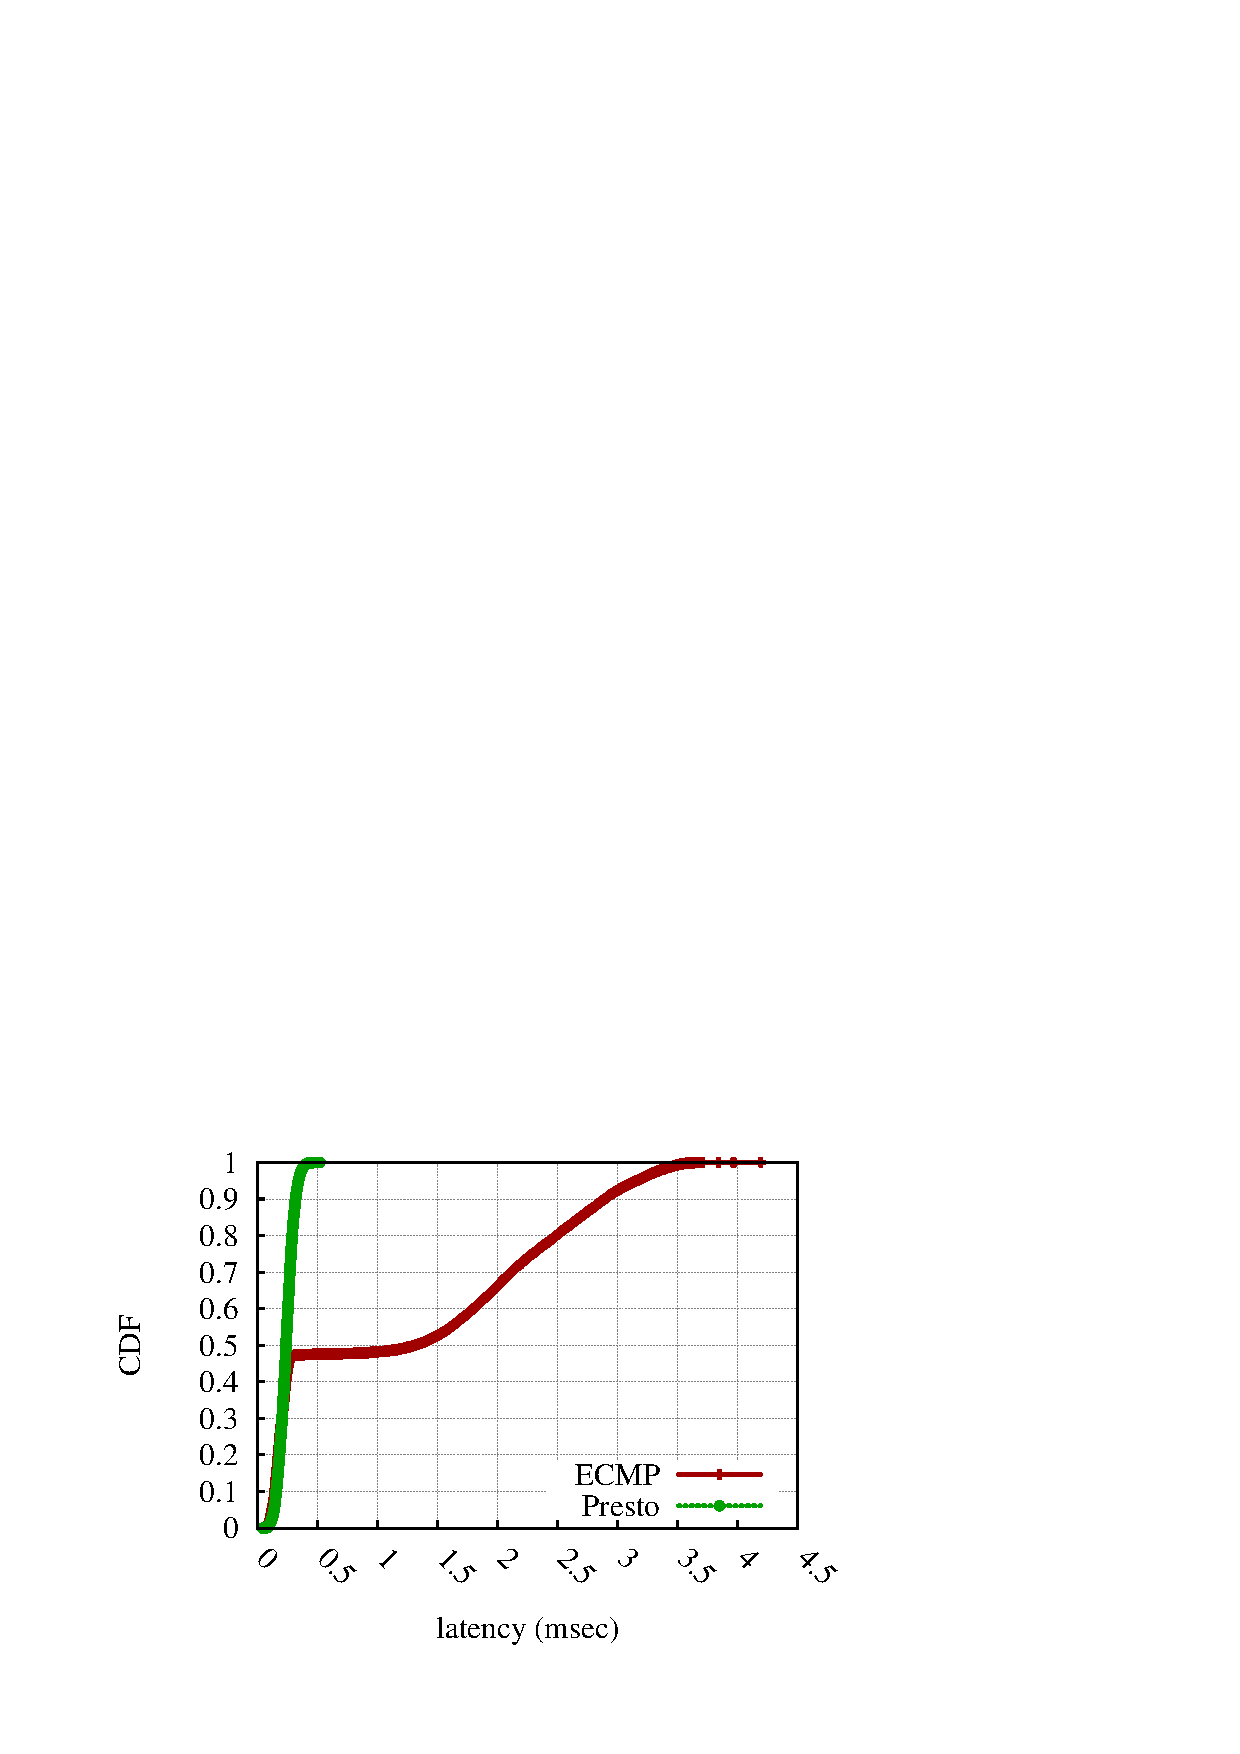
\includegraphics[width=0.45\textwidth]{presto/figures/scalability_test/scalability_compare_latency.pdf}
        \caption{Round trip time comparison in scalability benchmark. 
		%We increase the number of spine switches (i.e., the number of intermediate paths)
                %and set the number of flows (host pairs) equal to the number of available paths. 
		}
        \label{micro_scalability_test_latency}
\end{figure}


\begin{figure}[t]
        \centering
	\centering
        \begin{subfigure}[b]{0.225\textwidth}
                \centering
		\includegraphics[width=\textwidth]{presto/figures/scalability_test/scalability_compare_loss.pdf}
		\caption{}
		\label{micro_scalability_test_loss}
        \end{subfigure}
        \begin{subfigure}[b]{0.225\textwidth}
  		\includegraphics[width=\textwidth]{presto/figures/scalability_test/scalability_compare_fairness.pdf}
        	\caption{}
        	\label{micro_scalability_test_fairness}
	\end{subfigure}
	\caption{(a) Loss rate and (b) Fairness index comparison in scalability benchmark.}
\end{figure}

\tightparagraph{Presto Scales to Multiple Paths}
We analyze Presto's ability to scale in the number of paths by
setting the number of flows (host pairs) equal to the number of available paths in the topology shown in 
Figure~\ref{micro_scalability_topology}. The number of paths is varied from 2 to 8, and 
Presto always load-balances over all available paths.
Figure~\ref{micro_scalability_test_tput} shows Presto's throughput closely tracks Optimal. 
ECMP (and MPTCP) suffer from lower throughput when flows (or subflows) are
hashed to the same path. Hashing on the same path leads to congestion and thus increased latency, as shown in Figure~\ref{micro_scalability_test_latency}.
Because this topology is non-blocking and Presto load-balances in a near optimal fashion, Presto's latency
is near Optimal. Packet drop rates are presented in Figure~\ref{micro_scalability_test_loss} and show
Presto and Optimal have no loss. MPTCP has higher loss because of its bursty nature~\cite{conga}
and its aggression in the face of loss: when a single loss occurs, only
one subflow reduces its rate. The other schemes are more conservative because a single loss reduces the rate of the whole flow.
Finally, Figure~\ref{micro_scalability_test_fairness} shows Presto, Optimal and MPTCP
achieve almost perfect fairness.
%The underlying reason is that MPTCP makes traffic more bursty~\cite{conga}.


%%%congestion test figures %%%%
\begin{figure}[t]
        \centering
  \includegraphics[width=0.45\textwidth]{presto/figures/congestion_test/congestion_compare_tput_witherrbar.pdf}
        \caption{Throughput comparison in oversubscription benchmark.}
        \label{micro_congestion_test_tput}
\end{figure}


\begin{figure}[t]
        \centering
  \includegraphics[width=0.45\textwidth]{presto/figures/congestion_test/congestion_compare_latency.pdf}
        \caption{Round trip time comparison in oversubscription benchmark.
		}
        \label{micro_congestion_test_latency}
\end{figure}



\begin{figure}[t]
        \centering
	\centering
        \begin{subfigure}[b]{0.225\textwidth}
                \centering
		\includegraphics[width=\textwidth]{presto/figures/congestion_test/congestion_compare_loss.pdf}
		\caption{}
		\label{micro_congestion_test_loss}
	\end{subfigure}
	\begin{subfigure}[b]{0.225\textwidth}
		\centering
  		\includegraphics[width=\textwidth]{presto/figures/congestion_test/congestion_compare_fairness.pdf}
		\caption{}
        \label{micro_congestion_test_fairness}
	\end{subfigure}
	\caption{(a) Loss rate and (b) Fairness index comparison in oversubscription benchmark.}
\end{figure}

\tightparagraph{Presto Handles Congestion Gracefully}
Presto's ability to handle congestion is analyzed by fixing 
the number of spine and leaf switches to 2 and varying
the number of flows (host pairs) from 2 to 8, as shown
in Figure~\ref{micro_congestion_topology}. 
Each flow sends as much as possible, which leads to the network
being oversubscribed by a ratio of 1 (two flows) to 4 (eight flows).
Figure~\ref{micro_congestion_test_tput} shows all schemes track Optimal in highly
oversubscribed environments. ECMP
does poorly under moderate congestion because the limited number of flows can be hashed to the same path.
Presto does no worse in terms of latency (Figure~\ref{micro_congestion_test_latency}) and loss (Figure~\ref{micro_congestion_test_loss}).
The long tail latency for MPTCP is caused by its higher loss rates.
Both Presto and MPTCP have greatly improved fairness compared with ECMP (Figure~\ref{micro_congestion_test_fairness}).

\begin{figure}[!t]
        \centering
  \includegraphics[width=0.45\textwidth]{presto/figures/flowlets/flowlet_switching/flowlet_presto_compare_sockperf.pdf}
        \caption{Round trip time comparison of flowlet switching and Presto in Stride workload. 
		The throughputs of Flowlet switching with 100 $\mu\text{s}$ gap, 500 $\mu\text{s}$ gap and Presto 
		are 4.3 Gbps, 7.6 Gbps and 9.3 Gbps respectively. }
        \label{micro_flowlet_rtt_compare}
\end{figure}


\tightparagraph{Comparison to Flowlet Switching}
We first implemented a flowlet load-balancing scheme in OVS that detects
inactivity gaps and then schedules flowlets over disjoint paths in a round robin fashion.
%(Presto does this over flowcells instead of flowlets).
The receiver for flowlets uses official GRO.
Our flowlet scheme is not a direct reflection of CONGA because (i) it is not 
congestion-aware and (ii) the flowlets are determined in the software edge
instead of the networking hardware.
Presto is compared to 500 $\mu$s and 100 $\mu$s inactivity timers in
the stride workload on the 2-tier Clos network (Figure~\ref{macro_evaluation_topology}).
The throughput of the schemes are 9.3 Gbps (Presto), 7.6 Gbps (500 $\mu$s), and 4.3 Gbps (100 $\mu$s).
%Switching flowlets on very small timescales, such as 100$\mu$s, provides opportunities to create many flowlets.
%The largest flowlet is only 0.20\% (XX) of the total network traffic, which corresponds to about 5-9 MB in our runs.
%And while small flowlets create an even distribution
%of traffic over the network, significant strain is put on the TCP connection due to packet reordering. 
Analysis of the 100 $\mu$s
network traces show 13\%-29\% packets in the connection are reordered, which means 100 $\mu$s is not enough
time to allow packets to arrive in-order at the destination and thus throughput is severely impacted. Switching flowlets with 500 $\mu$s prevents
most reordering (only 0.03\%-0.5\% packets are reordered), but creates very large flowlets (see Figure~\ref{micro_flowlet_size}). This means
flowlets can still suffer from collisions, which can hurt throughput (note: while not shown here, 500 $\mu$s outperforms ECMP by over 40\%).
Figure~\ref{micro_flowlet_rtt_compare} shows the
latencies. Flowlet 100 $\mu$s has low throughput and hence lower latencies. However, since
its load balancing isn't perfect, it can still cause increased congestion in the tail. Flowlet 500 $\mu$s
also has larger tail latencies because of more pronounced flowlet collisions. As compared to the flowlet
schemes, Presto decreases 99.9$^{th}$ percentile latency by 2x-3.6x.
%Presto, by enforcing small flowlet sizes and explicitly accounting for reordering on the receiver, can obtain near
%line rate throughput with minimal tail latencies. 



%%%%presto 2 mods (ecmp and shaodw MAC) compare
\begin{figure}[!t]
        \centering
  \includegraphics[width=0.45\textwidth]{presto/figures/presto_compare_2modes/presto_compare_2mods.pdf}
        \caption{Round trip time comparison between Presto + shadow MAC and Presto + ECMP.
		%Compare Presto 2 modes' (Presto over ECMP and Presto over Shadow MAC) performance.
                %Simple 2-tier Clos network with 4 senders and 4 receivers, 4 paths between any host pair.
                %10 seconds per run, 20 runs. Use {\tt nuttcp} to measure throughput. Use {\tt sockperf}
                %to measure latency (RTT).
                %In Presto+ECMP, the average throughput is 7.9 (8.7 if trade latency for tput)
                %Gbps while in Presto+Shadow MAC, the
                %average throughput is 9.3Gbps 
		}
        \label{micro_presto_2mods}
\end{figure}

\tightparagraph{Comparison to Local, Per-Hop Load Balancing}
Presto sends flowcells in a round robin fashion over pre-configured end-to-end paths. An alternative is to
have ECMP hash on flowcell ID and thus provide per-hop load balancing. 
%One way to implement Presto + ECMP is to let vSwitch copy real TCP source port into a pre-allocated TCP option field 
%(\todo{this requires TCP stack allocates the new TCP option before sending to vSwitch}) and 
%encode chunk ID into TCP source port field. Because chunk ID is incremental, ECMP randomly maps chunks into multiple paths. 
We compare Presto + shadow MAC with Presto + ECMP using a stride workload on our testbed. 
Presto + shadow MAC's average throughput is 9.3 Gbps while Presto + ECMP's is 8.9 Gbps.
The round trip time CDF is shown in Figure~\ref{micro_presto_2mods}. 
Presto + shadow MAC gives better latency performance compared with Presto + ECMP. 
The performance difference comes from the fact that Presto + shadow MAC provides 
better fine-grained flowcell load balancing because 
randomization in per-hop multipathing can lead to corner cases where
a large fraction of flowcells get sent to the same link over a small timescale by multiple flows. This transient congestion
can lead to increased buffer occupancy and higher delays.

\subsection{Macrobenchmarks}
\label{macro}

%%%%%%%%%%using figures to present incast: tput, fariness, droprate, TCP RTT
\begin{figure}[!t]
        \centering
        \begin{subfigure}[b]{0.45\textwidth}
                \centering
                \includegraphics[width=\textwidth]{acdctcp/figures/incast/plots9k/incast_tput_vary_sender.pdf}
                \caption{Average throughput.}
                \label{incast_9k_tput}
        \end{subfigure}
        \begin{subfigure}[b]{0.45\textwidth}
                \centering
                \includegraphics[width=\textwidth]{acdctcp/figures/incast/plots9k/incast_fairness_vary_sender.pdf}
                \caption{Fairness.}
                \label{incast_9k_fariness}
        \end{subfigure}
        \caption{Many to one incast: throughput and fairness.}
        \label{incast_9k_tput_fairness}
\end{figure}

\begin{figure*}[!t]
        \centering
        \begin{subfigure}[b]{0.3\textwidth}
                \centering
                \includegraphics[width=\textwidth]{acdctcp/figures/incast/plots9k/incast_sockperf50th_vary_sender.pdf}
                \caption{50$^{th}$ percentile RTT.}
                \label{incast_9k_50th_sockperf}
        \end{subfigure}
        \begin{subfigure}[b]{0.3\textwidth}
                \centering
                \includegraphics[width=\textwidth]{acdctcp/figures/incast/plots9k/incast_sockperf999th_vary_sender.pdf}
                \caption{99.9$^{th}$ percentile RTT.}
                \label{incast_9k_999th_sockperf}
        \end{subfigure}
        \begin{subfigure}[b]{0.3\textwidth}
                \centering
                \includegraphics[width=\textwidth]{acdctcp/figures/incast/plots9k/incast_droprate_vary_sender.pdf}
                \caption{Packet drop rate.}
                \label{incast_9k_droprate}
        \end{subfigure}
        \caption{Many to one incast: RTT and packet drop rate.\crs{~\acdc{} can reduce DCTCP's RTT by limiting window sizes.}}
        \label{incast_9k_sockperf_droprate}
\end{figure*}


\begin{figure}[!t]
        \centering
  \includegraphics[width=0.5\textwidth]{acdctcp/figures/incast/pressure/incast_pressure_compare_sockperf.pdf}
        \caption{TCP RTT when almost all ports are congested.}
        \label{sockperf_pressure_incast}
\end{figure}

%
%

\iffalse
\begin{figure*}[!t]
        \centering
        \begin{subfigure}[b]{0.45\textwidth}
                \centering
                \includegraphics[width=\textwidth]{acdctcp/figures/macro_benchmarks/macro_4stride/stride4_mice16KB_fct.pdf}
                \caption{Mice flow completion times.}
                \label{macro_4stride_mice_fct}
        \end{subfigure}
        \begin{subfigure}[b]{0.45\textwidth}
                \centering
                \includegraphics[width=\textwidth]{acdctcp/figures/macro_benchmarks/macro_4stride/stride4_big512MB_fct.pdf}
                \caption{Background flow completion times.}
                \label{macro_4stride_background_fct}
        \end{subfigure}
        \caption{CDF of mice and background FCTs in concurrent stride workload.}
        \label{macro_4stride_fct}
\end{figure*}

\begin{figure*}[!t]
        \centering
        \begin{subfigure}[b]{0.45\textwidth}
                \centering
                \includegraphics[width=\textwidth]{acdctcp/figures/macro_benchmarks/shuffle_17hosts/shuffle_mice16KB_fct.pdf}
                \caption{Mice flow completion times.}
                \label{macro_shuffle_mice_fct}
        \end{subfigure}
        \begin{subfigure}[b]{0.45\textwidth}
                \centering
                \includegraphics[width=\textwidth]{acdctcp/figures/macro_benchmarks/shuffle_17hosts/shuffle_big512MB_fct.pdf}
                \caption{Background flow completion times.}
                \label{macro_shuffle_background_fct}
        \end{subfigure}
        \caption{CDF of mice and background FCTs in shuffle workload.}
        \label{macro_shuffle_fct}
\end{figure*}

\begin{figure*}[!t]
        \centering
        \begin{subfigure}[b]{0.45\textwidth}
                \centering
                \includegraphics[width=\textwidth]{acdctcp/figures/macro_benchmarks/trace-driven/trace_driven_workload_dctcp_senders5_10points.pdf}
                \caption{Web-search workload.}
                \label{trace-driven-searching-fct}
        \end{subfigure}
        \begin{subfigure}[b]{0.45\textwidth}
                \centering
                \includegraphics[width=\textwidth]{acdctcp/figures/macro_benchmarks/trace-driven/trace_driven_workload_conga_senders5_10points.pdf}
                \caption{Data-mining workload.}
                \label{trace-driven-data-mining-fct}
        \end{subfigure}
        \caption{CDF of mice ($<$10KB) FCT in web-search and data-mining workloads.}
        \label{macro-trace-driven-fct}
\end{figure*}
\fi


In this section we attach all servers to a single switch and
run a variety of workloads to better understand
how well~\acdc{} tracks DCTCP's performance. Experiments are run for 10 minutes. A simple TCP application
sends messages of specified sizes to measure FCTs.

\tightparagraph{Incast}
In this section, we evaluate incast scenarios.
To scale the experiment, 17 physical servers are equipped with four NICs each
and one flow is allocated per NIC.
In this way, incast can support up to 47-to-1 fan-in (our switch only has 48 ports).
We measure the extent of incast by increasing the number of concurrent senders to 16, 32, 40 and 47.
Figure~\ref{incast_9k_tput_fairness} shows throughput and fairness results.
Both DCTCP and \acdc{} obtain a fairness index greater than 0.99 and get comparable throughput as CUBIC.
Figure~\ref{incast_9k_sockperf_droprate} shows the RTT and packet drop rate results.
When there are 47 concurrent senders, DCTCP can reduce median RTT by 82\% and \acdc{} can reduce by 97\%;
DCTCP can reduce 99.9$^{th}$ percentile RTT by 94\% and \acdc{} can reduce by 98\%.
Both DCTCP and \acdc{} have 0\% packet drop rate. It is curious that~\acdc{}’s
performance is better than DCTCP when the number of senders increases (Figure~\ref{incast_9k_50th_sockperf}).
The Linux DCTCP code puts a lower bound of 2 packets on \cwnd{}.
In incast, we have up to 47 concurrent competing flows and
the network's MTU size is 9KB. In this case, the lower bound is too high,
so DCTCP's RTT increases gradually with the number of senders.
This issue was also found in~\cite{judd2015nsdi}.~\acdc{} controls \rwnd{} (which is in bytes)
instead of \cwnd{} (which is in packets) and \rwnd{}'s lowest value can be much smaller than 2*MSS.
We verified modifying~\acdc{}'s lower bound caused identical behavior.

\crs{The second test aims to put pressure on the switch's dynamic
buffer allocation scheme, similar to an experiment in the DCTCP paper~\cite{alizadeh2011data}.}
To this end, we aim to congest every switch port.
The 48 NICs are split into 2 groups: group $A$ and $B$.
Group $A$ has 46 NICs and $B$ has 2 (denoted $B_1$ and $B_2$).
Each of the 46 NICs in $A$ sends and receives 4 concurrent flows within $A$
(\ie{}, NIC $i$ sends to [$i+1$, $i+4$] mod 46).
Meanwhile, all of the NICs in $A$ send to $B_1$, creating a 46-to-1 incast.
This workload congests 47 out of 48 switch ports.
We measure the RTT between $B_2$ and $B_1$ (i.e., RTT of the traffic traversing the most congested port) and
the results are shown in Figure~\ref{sockperf_pressure_incast}.
The average throughputs for CUBIC, DCTCP, and~\acdc{} are 214, 214 and 201 Mbps respectively,
all with a fairness index greater than 0.98.
CUBIC has an average drop rate of 0.34\% but the most congested port has a drop rate as high as 4\%.
This is why the 99.9$^{th}$ percentile RTT for CUBIC is very high.
The packet drop rate for both DCTCP and~\acdc{} is 0\%.

\begin{figure*}[!t]
        \centering
        \begin{subfigure}[b]{0.45\textwidth}
                \centering
                \includegraphics[width=\textwidth]{acdctcp/figures/macro_benchmarks/macro_4stride/stride4_mice16KB_fct.pdf}
                \caption{Mice flow completion times.}
                \label{macro_4stride_mice_fct}
        \end{subfigure}
        \begin{subfigure}[b]{0.45\textwidth}
                \centering
                \includegraphics[width=\textwidth]{acdctcp/figures/macro_benchmarks/macro_4stride/stride4_big512MB_fct.pdf}
                \caption{Background flow completion times.}
                \label{macro_4stride_background_fct}
        \end{subfigure}
        \caption{CDF of mice and background FCTs in concurrent stride workload.}
        \label{macro_4stride_fct}
\end{figure*}

\begin{figure*}[!t]
        \centering
        \begin{subfigure}[b]{0.45\textwidth}
                \centering
                \includegraphics[width=\textwidth]{acdctcp/figures/macro_benchmarks/shuffle_17hosts/shuffle_mice16KB_fct.pdf}
                \caption{Mice flow completion times.}
                \label{macro_shuffle_mice_fct}
        \end{subfigure}
        \begin{subfigure}[b]{0.45\textwidth}
                \centering
                \includegraphics[width=\textwidth]{acdctcp/figures/macro_benchmarks/shuffle_17hosts/shuffle_big512MB_fct.pdf}
                \caption{Background flow completion times.}
                \label{macro_shuffle_background_fct}
        \end{subfigure}
        \caption{CDF of mice and background FCTs in shuffle workload.}
        \label{macro_shuffle_fct}
\end{figure*}

\begin{figure*}[!t]
        \centering
        \begin{subfigure}[b]{0.45\textwidth}
                \centering
                \includegraphics[width=\textwidth]{acdctcp/figures/macro_benchmarks/trace-driven/trace_driven_workload_dctcp_senders5_10points.pdf}
                \caption{Web-search workload.}
                \label{trace-driven-searching-fct}
        \end{subfigure}
        \begin{subfigure}[b]{0.45\textwidth}
                \centering
                \includegraphics[width=\textwidth]{acdctcp/figures/macro_benchmarks/trace-driven/trace_driven_workload_conga_senders5_10points.pdf}
                \caption{Data-mining workload.}
                \label{trace-driven-data-mining-fct}
        \end{subfigure}
        \caption{CDF of mice (flows$<$10KB) FCT in web-search and data-mining workloads.}
        \label{macro-trace-driven-fct}
\end{figure*}

\tightparagraph{Concurrent stride workload}
In concurrent stride, 17 servers are attached to a single switch.
Each server $i$ sends a 512MB flow to servers [$i+1$, $i+4$] mod 17 in sequential fashion
to emulate background traffic.
Simultaneously, each server $i$ sends 16KB messages every 100 ms to 
server $(i+8)$ mod 17.
The FCT for small flows (16KB) and background flows (512MB) are shown 
in Figure~\ref{macro_4stride_fct}. For small flows, DCTCP and \acdc{} 
reduce the median FCT by 77\% and 76\% respectively. 
At the 99.9$^{th}$ percentile, DCTCP and \acdc{} reduce FCT by 91\% and 93\%, respectively.
For background flows, DCTCP and \acdc{} offer similar completion times.
CUBIC has longer background FCT because its fairness is not as 
good as DCTCP and \acdc{}.


\tightparagraph{Shuffle workload}
In shuffle, each server sends 512MB to every other server in random order. 
A sender sends at most 2 flows simultaneously and when
a transfer is finished, the next one is started until 
all transfers complete.
Every server $i$ also sends a 16 KB message to server $(i+8)$ mod 17 
every 100 ms. This workload is repeated for 30 runs.
The FCT for each type of flow is shown in Figure~\ref{macro_shuffle_fct}.
For small flows, DCTCP and \acdc{} reduce median FCT by
72\% and 71\% when compared to CUBIC. 
At the 99.9$^{th}$ percentile, DCTCP and \acdc{} 
reduce FCTs by 55\% and 73\% respectively.
For large flows, CUBIC, DCTCP and \acdc{} have almost identical performance.


\tightparagraph{Trace-driven workloads}
Finally, we run trace-driven workloads. 
An application on each server builds a long-lived TCP connection with every other server.
Message sizes are sampled from a trace and sent to a random destination in sequential fashion. Five
concurrent applications on each server are run to increase network load. Message
sizes are sampled from a web-search~\cite{alizadeh2011data}
and a data-mining workload~\cite{greenberg2009vl2,alizadeh2014conga}, whose flow size distribution has a heavier tail.
Figure~\ref{macro-trace-driven-fct} shows a CDF of FCTs for mice flows (smaller than 10KB) 
in the web-search and data-mining workloads.
In the web-search workload,
DCTCP and \acdc{} reduce median FCTs by 77\% and 76\%, respectively. 
At the 99.9$^{th}$ percentile, DCTCP and \acdc{} reduce FCTs by 50\% and 55\%, respectively.
In the data-mining workload, DCTCP and \acdc{} reduce median FCTs by 72\% and 73\%, respectively. 
At the 99.9$^{th}$ percentile, DCTCP and \acdc{} reduce FCTs by 36\% and 53\% respectively.  
%In both workloads, DCTCP and \acdc{} improve the fraction of mice flows that finish 
%in 1 millisecond significantly (from 20\%/30\% to 80\%).

\tightparagraph{Evaluation summary}
The results validate that congestion control can be accurately implemented in the vSwitch.
~\acdc{} tracks the performance of an unmodified host DCTCP stack
over a variety of workloads with little computational overhead.
Furthermore,~\acdc{} provides this functionality over 
various host TCP congestion control configurations. 


%\section{Discussion}
\label{discuss}

\tightparagraph{UDP traffic} How to handle. 
Mention VxLAN traffic too.
\keqiang{and IPsec}

\tightparagraph{No vSwitch} 
\keqiang{title should be hypervisor-bypass?}
Use middleboxes (for DB server).
Use NIC (for SR-IOV).
Hypervisor bypass (e.g., SR-IOV), where TCP traffic is sent to the NIC directly without 
going through hypervisor. First, as noted by~\cite{shieh2011sharing}, ``loss of the security and 
manageability features provided by the software virtual switch has limited 
the deployment of direct I/O NICs in public clouds''. Second, based on techniques like Intel 
DPDK~\cite{intel-dpdk} and ``smart NICs''~\cite{cavium-nic,netronome-nic}, we believe that low latency 
congestion control enforcement schemes like \acdc{} can also be 
employed for hypervisor bypass use cases.
We need to worry about legacy systems and non-VM systems. For instance, a database or storage device that may not have OVS installed on it.
We need to talk about either a middlebox or that this percentage of traffic is low? Or implement in NIC (especially one with OVS offload?).

\tightparagraph{North-South traffic.}
Transport enforcement should be only be done for east west traffic, so if the tenant tuned their stack's
congestion control algorithm for wide-area networks, their north sourth traffic is not affected and their 
congestion control scheme can still achieve good performance.

\keqiang{todos: some figures do not read well on printed paper}
\keqiang{todos: sometimes, when we refer a section, we say ``Section X'', sometimes, we use the 
dollar sign, we should unify them}

%
%Byzantine VM.
%
%Other names: ACDCTCP, LiquidSwitch, LiquidEdge
%
%In CPU overhead measurement, we need to 
%mention ovs add 1 widecard rule. That means we isolated the overhead of 
%OVS itself when it has many flows in its flow table (probably it does not matter
%at the end of the day, because we measured the CPU usage of the whole system).
%
%People may say window-based congestion control is burty. TIMELY operates 
%on TCP segments in order to reduce CPU overhead. Therefore, TIMELY is also
%busty. In TIMELY, they mentioned they can leverage a hybrid scheme, that is
%using software to control large segments and use hardware rate limiter to
%reduce burstyness.
%
%Create loss and check how DCTCP and our scheme treates packet losses (revisit it after we finish incast 
%and macrobenchmarks).
%
%One more microbenchmark on the Dumbbell topology: different servers have different transport, so the
%throughput fairness among different transports (e.g., start cubic, start New Reno, start dctcp).
%
%A point that is missing in DCTCP and NSDI paper is that they did not mention how the switch should be
%configured to handle non-TCP traffic. Note non-TCP traffic such as DNS (UDP 53) and ARP, ICMP etc
%are also important. We found that if we did not specify how the switch handle the non-TCP traffic,
%then this kind of non-TCP traffic can be easily dropped by the switch. We found ARP traffic is dropped
%by the switch such that DCTCP flows stall. Hence, we think it is better to put non-TCP traffic
%into a different queue when we apply WRED/ECN on the switches.
%
%This work offers low latency for ``hetergeneous networks" where different entities can 
%run different kinds of
%transport congestion control schemes. A few examples of such hetergeneous networks: public 
%datacenters where tenants can set up their own VMs (e.g., AWS), or tenants can rent their bare metal
%machines (e.g., SoftLayer), or certain groups (even within a single organization) 
%have to use traditional transports due to compatibility of legacy applications (NSDI's Judd said this), or
%incremental deployment is undergoing. 
%To ensure a pure low latency datacenter network, a universal transport enforcement scheme is required. 
%Two challenges to implement such a transport enforcement scheme are scalability and low overhead. 
%The transport enformancement scheme proposed here meet the two metrics (as shown in our experiments) while
%providing nice network performance (throughput, latency and packet drop rate). This scheme is 
%compatible with any kind of TCP stack. Finally, the scheme we propose solves the co-existence issue of 
%ECT (ECN Capable Transport) and non-ECT, which is a critical deployment hurdle for DCTCP-like transports.
%
%Macrobenchmark plan: 18 hosts, 6 switches, ECMP configured. The network oversubscription ratio is 2:1.
%Run all-to-all traffic for a long time (e.g., 1 hours). Show total throughput and TCP RTT and packet drop 
%rate.
%
%QoS can be implemented too?
%
%
%
%When we try to launch an instance in EC2: ``An AMI is a template that contains the software 
%configuration (operating system, application server, and applications) required to launch your instance. 
%You can select an AMI provided by AWS, our user community, or the AWS Marketplace; 
%or you can select one of your own AMIs''. Default is CUBIC for most Linux images, Window Servers can
%have NewReno, Compound TCP (CTCP)~\cite{tan2006compound} and DCTCP. 
%Users can tweak congestion control algorithms to optimize network performance for their target scenarios. 
%
%Section talking about how to implement other CC schemes: TIMELY, PERC, Vegas, etc.
%
%EJR: VXLAN, UDP, TCP stack statistics for Cloud?
%
%ECT and non-ECT: througput unfairness, long RTT, connection establishment..
%
%
%EyeQ, Seawall, NetShare, Silo, SecondNet, Oktopus etc. Our work did not provide bandwidth allocation property. 
%This work focused on reducing in-network queuing latency caused by VM TCP stacks. 
%We show how this goal can be done using a simple and elegant solution.
%Yes, if an VM opens more connections than another, that VM gains more bandwidth. 
%But, there are proposals which try to provide proper bandwidth allocation when multiple end-points compete 
%at the sender side or receiver side. Those works and this work are complementary. 
%To the best of our knowledge, today's cloud providers have not provide strong bandwidth guarantees 
%(for example, AWS only roughly classify VMs instances' network performance into 
%``low to moderate", ``moderate", ``high" and ``10 Gigabit"categories).
%
%talk about containers?

%\section{Related Work}
\label{related}
This section discusses different classes of related work.

\tightparagraph{Congestion control for DCNs}
\crs{Rather than proposing a new congestion control algorithm, our work investigates if congestion control can be moved to the vSwitch.
Thus, many of the following schemes are complimentary.}
DCTCP~\cite{dctcp} is a seminal TCP variant for datacenter networks.
Judd~\cite{judd2015nsdi} proposed simple yet practical fixes to enable DCTCP in production networks.
TCP-Bolt~\cite{stephens2014practical} is a variant of DCTCP for PFC-enabled lossless Ethernet.
%DCQCN~\cite{zhu2015congestion} is a rate-based congestion control scheme implemented in NICs
%for QCN-based~\cite{qcn} RDMA deployments.
DCQCN~\cite{zhu2015congestion} is a rate-based congestion control scheme (built on DCTCP and QCN) to
support RDMA deployments in PFC-enabled lossless networks.
TIMELY~\cite{mittal2015timely} and DX~\cite{lee2015accurate} 
use accurate network latency as the signal to perform congestion control.
TCP ex Machina~\cite{winstein2013tcp} uses computer-generated congestion control rules.
PERC~\cite{jose2015high} proposes proactive congestion control to improve convergence.
ICTCP's~\cite{wu2010ictcp} receiver monitors incoming TCP flows and 
modifies~\rwnd{} to mitigate the impact of incast, but this cannot
provide generalized congestion control like~\acdc{}.
Finally, efforts~\cite{dell-toe,chelsio-toe} to 
implement TCP Offload Engine (TOE) in specialized NICs are not widely deployed for reasons noted in~\cite{mogul2003tcp,linux-toe}.
%~\acdc{} is designed to work with commodity NICs. 

\tightparagraph{Bandwidth allocation} Many bandwidth allocation schemes have been proposed.
Gatekeeper~\cite{rodrigues2011gatekeeper} and EyeQ~\cite{jeyakumar2013eyeq} abstract the network as a single
switch and provide bandwidth guarantees by managing each server's access link.
Oktopus~\cite{Ballani2011oktopus} provides fixed performance guarantees within virtual clusters.
SecondNet~\cite{Guo2010Secondnet} enables virtual datacenters with static bandwidth guarantees.
Proteus~\cite{Xie2012Proteus} allocates bandwidth for applications with dynamic demands.
Seawall~\cite{shieh2011sharing} provides bandwidth proportional to a defined weight by
forcing traffic through congestion-based edge-to-edge tunnels. 
NetShare~\cite{Lam2012NetShare} utilizes hierarchical weighted max-min fair sharing to tune relative bandwidth allocation for services.
FairCloud~\cite{Popa2012Faircloud} identifies trade-offs in minimum
guarantees, proportionality and high utilization, and designs schemes over this space.
Silo~\cite{jang2015silo} provides guaranteed bandwidth, delay and burst allowances through a novel VM placement and admission 
algorithm, coupled with a fine-grained packet pacer. As discussed in~\sref{background}, 
~\acdc{} is largely complimentary to these schemes because it is a transport-level solution.

\tightparagraph{Rate limiters} 
SENIC~\cite{niranjan2013fastrak} 
identifies the limitations of NIC hardware rate limiters (\ie{}not scalable) and 
software rate limiters (\ie{}high CPU overhead) and uses the CPU to enqueue packets 
in host memory and the NIC. Silo's pacer injects void packets into 
an original packet sequence to achieve pacing. FasTrack~\cite{niranjan2013fastrak} offloads
functionality from the server into the switch for certain flows.~\acdc{} prevents
TCP flows from sending in the first place and can be used in conjunction with these
schemes.


\tightparagraph{Low latency DCNs}
Many schemes have been proposed to reduce latency in datacenter networks.
HULL~\cite{alizadeh2012less} uses phantom queues to leave bandwidth headroom to support low latency.
pFabric~\cite{alizadeh2013pfabric} is a clean-slate
design which utilizes priority and minimal switch buffering to achieve low latency.
Fastpass~\cite{perry2014fastpass} uses a centralized arbiter to
perform per-packet level scheduling.
QJUMP~\cite{qjump} uses priority queueing and rate limiting to
bound latency. Traffic engineering~\cite{hedera,rasley2014planck} and 
load balancing~\cite{conga,he2015presto,ghorbani2015micro} can also
reduce latency. Because~\acdc{} works on the transport level, it is
largely complimentary to these works.

\tightparagraph{Performance-enhancing proxies}
Several schemes improve end-to-end protocol performance via a middlebox
or proxy~\cite{RFC3449,RFC3115,balakrishnan2008maelstrom,davern2011httpep,balakrishnan1995improving}.
\acdc{} fits into this class of works, but is unique in providing a mechanism
to alter a VM's TCP congestion control algorithm by modifying the vSwitch.

\tightparagraph{Virtualized congestion control}
\crs{vCC~\cite{vcc} is a concurrently designed system that shares~\acdc{}'s goals and some of its design details.
The paper is complementary in that some items not addressed in this work are presented, such as a more detailed
analysis of the ECN-coexistence problem, an exploration of the design space, and a theoretical proof of
virtualized congestion control's correctness. Our paper provides an in-depth design and thorough evaluation of
a DCTCP-based virtualized congestion control algorithm on a 10 Gbps testbed.
}

\section{Summary}
Today's datacenters host a variety of VMs (virtual machines) in order to
support a diverse set of tenant services. Datacenter operators
typically invest significant resources in optimizing their network fabric,
but they cannot control one of the most important components of 
avoiding congestion: TCP's congestion control algorithm in the VM. In this chapter,
we present a technology that allows administrators to regain control over arbitrary tenant TCP stacks by enforcing congestion
control in the vSwitch. Our scheme, called~\acdc{} TCP, requires no 
changes to VMs or network hardware. Our approach is scalable, light-weight,
flexible and provides a policing mechanism to deal with non-conforming flows.
In our evaluation the CPU overhead is less than~\crs{one percentage point} and our scheme 
is shown to effectively enforce an administrator-defined congestion control
algorithm over a variety of tenant TCP stacks.





\chapter{Low Latency Software Rate Limiters for Cloud Networks}
\label{thesis:chapter:rate_limiter}

\chapter{Low Latency Software Rate Limiters for Cloud Networks}
\label{thesis:chapter:rate_limiter}

\section{Introduction}
\label{rate-limiter:sec:introduction}

Bandwidth allocation is an indispensable feature in multi-tenant clouds. 
It guarantees the performance of various applications from multiple tenants running on the same physical server. 
Bandwidth allocation is often implemented by \textit{software rate limiters\footnote{In this chapter,
we use software rate limiter and rate limiter interchangeably.}} 
in the operating system (e.g., Linux Hierarchical Token Bucket, aka HTB) due to their flexibility and scalability.
However, rate limiters either uses traffic policing (i.e., dropping packets when
packet arrival rate is above the desired rate) or traffic shaping (i.e., queueing packets in a large
queue to absorb burst and send packets to the network based on token and bucket algorithms).
Thus, bandwidth allocation, low latency and low loss rate can be not achieved at the same time. 
We conduct performance measurements in a public cloud platform (CloudLab~\cite{cloudlab}) and 
find that one of the most widely used software rate limiters, HTB, dramatically increases network latency.

Previous work mainly focused on solving ``in-network'' queueing latency (i.e., latency in 
switches)~\cite{alizadeh2010data,he2016ac,mittal2015timely}, but little research effort has been
done to solve the latency, packet loss and burstiness issues for the software rate limiters on the end-host.
To this end, we explore how we can address the performance issues associated with rate limiters on the end-host in this chapter.
Inspired by the efforts to reduce queueing latency in hardware switches, 
we first extend ECN into software rate limiters and configure DCTCP on the end-points. 
However, in our tests, we find simply applying DCTCP+ECN on the end-host causes a problem \textemdash\xspace 
TCP throughput tends to oscillate (between 50\% to 95\% in some cases, see Section~\ref{rate-limiter:sec:measurement}). 
And throughput oscillation would significantly degrade application performance. 

There are two issues with simply applying DCTCP+ECN on end-host rate limiters. The first is that, different from
hardware switches in the network, end-hosts process TCP segments instead of MTU-sized packets. 
TCP Segmentation Offload (TSO)~\cite{tcp-segment-offload} is an optimization technique 
that is widely used in modern operating systems to reduce CPU overhead
for fast speed networks. TSO is enabled in Linux by default. Because of TSO, TCP segment size can reach
64KB in the default setting. That means, if we mark the ECN bits in one TCP segment, a bunch of 
consecutive MTU-sized packets are marked because the ECN bits in the header are copied into each packet in the NIC.
On the other hand, if a TCP segment is not marked, then none of the packets in this segment is marked. This kind of 
coarse-grained segment-level marking leads to an inaccurate estimation of congestion level, and consequently 
leads to throughput oscillation.
The second issue with DCTCP+ECN is that its congestion control loop latency is large. There are three types of 
traffic in datacenter networks \textemdash\xspace 1) intra-datacenter traffic (i.e., east-west traffic) 2) inter-datacenter
traffic and 3) traffic that goes across WANs to remote clients. DCTCP+ECN's control loop latency is one RTT.
But RTT is affected by many factors. For intra-datacenter traffic, RTT is affected by ``in-network'' congestion.
For traffic that goes across WANs to remote clients, its RTT can be tens of milliseconds.
Congestion control loop latency is not bounded and congestion control actions can rely on stale congestion feedback.
The long congestion control loop latency is further exacerbated by the fact that traffic on the end-host is bursty
because of TCP windowing scheme and TSO optimizations~\cite{kapoor2013bullet}.


To address the shortcomings of DCTCP+ECN, 
we design our first mechanism \textemdash\xspace \textit{direct ECE marking (\nameone)}. 
In \nameone, when an ACK is received, \nameone checks the real-time queue length in its corresponding rate limiter, 
and if the queue length exceeds a pre-configured threshold, \nameone \textit{marks the ACK packet instead of data packets}. 
By marking TCP ACK, we mean set TCP ACK's ECN-Echo (ECE) bit.
Directly marking TCP ECE avoids the two shortcomings in DCTCP+ECN. First, the congestion control loop
latency is almost reduced to 0 because it is based on real-time queue length, not the queue length one RTT ago.
Second, it avoids coarse-grained segment-level ECN marking on the transmitting path.
Our design (Section~\ref{rate-limiter:sec:design}) and experiment (Section~\ref{rate-limiter:sec:evaluation}) show that 
DEM eliminates throughput oscillation.
 

There is a prerequisite to deploying \nameone \textemdash\xspace end-hosts are able to react to ECN marking correctly 
(e.g., DCTCP). However, in public clouds, this prerequisite does not always hold 
because the cloud operator does not have access to the network stack configuration in tenants' VMs. 
Even the tenant VM is configured with DCTCP, not all the flows are ECN-capable. For example,
TCP flows between cloud and clients are usually not ECN-capable because ECN is not widely used in WANs~\cite{kuhlewind2013state}.
To make our solution more generic, we adopt the mechanism from AC/DC~\cite{he2016ac}, 
i.e., performing TCP \cwnd computation outside of tenants' VMs and enforcing congestion control decisions via 
rewriting \rwnd. We also design and implement a window-based TIMELY~\cite{mittal2015timely}-like congestion control algorithm. 
We name this mechanism \nametwo. \nametwo completely gets rid of ECN marking and can work for 
both ECN-capable and non ECN-capable flows. 
\nametwo also avoids the two issues that DCTCP+ECN has because for each return ACK, 
we compute \cwnd according to instantaneous rate limiter queue length and queue length gradient and 
rewrite \rwnd in TCP ACK header. 

The contributions of this chapter are as follows:
\begin{enumerate}
\item We point out and measure the latency caused by software rate limiters on the end-host in multi-tenant clouds, 
and also show that simply applying DCTCP+ECN is not sufficient to achieve constant bandwidth saturation.

\item We identify the limitations of DCTCP+ECN in end-host networking and 
propose \nameone to solve the throughput oscillation problem.
We also propose \nametwo to make the solution more generic and deployable.

\item We perform a preliminary evaluation to show our solutions can achieve high bandwidth saturation, 
low latency, low oscillation and throughput fairness with negligible CPU overhead.

\iffalse
\item We measure the performance (latency and packet loss) of software rate limiters. We show that software rate limiters can greatly increase end-to-end latency for multi-tenant cloud networks. 
We also show that simply extending ECN in software rate limiter queues and enabling DCTCP on the end-points (i.e., VMs or Container) give sub-optimal performance. 

\item We propose two techniques (\nameone and \nametwo) to enable high throughput, low oscillation, low latency and generic software rate limiters for multi-tenant cloud networks.

\item We evaluate the performance of \nameone and \nametwo. The experiment results demonstrate that the proposed solutions achieve our design goals.
\fi
\end{enumerate}


\section{Background and Motivation}
\label{background}
This section first gives a brief background of congestion 
control in the datacenter. Then the motivation for moving congestion
control into the vSwitch is presented. Finally,~\acdc{} is contrasted from a class of related bandwidth
allocation schemes.

\subsection{Datacenter Transport}
\label{ss:dct}
Today's datacenters host applications such as search,
advertising, analytics and retail that require high bandwidth and low latency.
%Large tail latencies often violate the tight timing constraints required by SLAs at scale, and
%have been shown to impact customer experience, result in
%revenue loss~\cite{alizadeh2011data,dean2013tail}, and degrade application performance~\cite{jang2015silo,qjump}.
%Tail latencies are often caused by network congestion.
%The latency of traversing a single switch, NIC and OS network stack is 10--30$\mu$s,
%2.5--32$\mu$s and 15$\mu$s respectively, but a congested port
%on a network switch can consume significant shared memory, causing orders-of-magnitude
%higer latency~\cite{rumble2011s}.
Network congestion, caused by imperfect load balancing~\cite{al2010hedera},
network upgrades or failures, can adversely impact these services. Unfortunately, congestion is
not rare in datacenters. For example, recently Google reported 
congestion-based drops were observed when network utilization approached 25\%~\cite{singh2015jupiter}.
Other studies have shown high variance and substantial increase in the 99.9$^{th}$ percentile latency
for round-trip times in today's datacenters~\cite{wang2010impact,mogul2015inferring}. 
Large tail latencies impact customer experience, result in
revenue loss~\cite{alizadeh2011data,dean2013tail}, and degrade application performance~\cite{jang2015silo,qjump}.
Therefore, significant motivation exists to reduce congestion in datacenter fabrics.

%Studies have shown that while CUBIC can achieve
%high bandwidth, it does so at the cost of aggressively filling up the switch buffers in the network.
TCP's congestion control algorithm is
known to significantly impact network performance.
As a result, datacenter TCP performance has been widely
studied and many new protocols have been proposed~\cite{alizadeh2011data, stephens2014practical, wu2010ictcp,
mittal2015timely, jose2015high}. Specifically, DCTCP~\cite{alizadeh2011data} adjusts a TCP sender's rate based on the fraction of packets experiencing congestion. In DCTCP,
the switches are configured to mark packets with an ECN bit when their queue lengths exceed a threshold. By proportionally
adjusting the rate of the sender based on the fraction of ECN bits received, DCTCP can keep queue lengths low, 
maintain high throughput, and increase fairness and stability over traditional schemes~\cite{alizadeh2011data,judd2015nsdi}.
\crs{For these reasons, we implement DCTCP as the vSwitch congestion control algorithm in~\acdc{}.}

\subsection{Benefits of~\acdc{}}
%Rather than proposing a new datacenter congestion control algorithm, this work investigates
%if congestion control can be moved to the vSwitch.
Allowing administrators to enforce an optimized congestion control without
changing the VM is the first major benefit of our scheme.
This is an important criteria in untrusted public cloud environments or simply in cases where servers cannot be updated
due to a dependence on a specific OS or library.~\cite{judd2015nsdi}


\begin{figure}[!t]
        \centering
        \begin{subfigure}[b]{0.45\textwidth}
                \centering
		%max min mean median
                %\includegraphics[width=\textwidth]{acdctcp/figures/tput_fairness/default_5CC_tput.pdf}
                %5 CCs
		\includegraphics[width=\textwidth]{acdctcp/figures/tput_fairness/default_5CC_tput_detail.pdf}
		\caption{5 different CCs.}
                \label{unfairness_5CC}
        \end{subfigure}
        \begin{subfigure}[b]{0.45\textwidth}
                \centering
                \includegraphics[width=\textwidth]{acdctcp/figures/tput_fairness/default_all_cubic_tput.pdf}
                \caption{All CUBIC.}
                \label{unfairness_all_cubic}
        \end{subfigure}
%        \begin{subfigure}[b]{0.24\textwidth}
%                \centering
%                \includegraphics[width=\textwidth]{acdctcp/figures/tput_fairness/liquid_5CC_tput.pdf}
%                \caption{5 different CCs with \acdc{}.}
%                \label{fairness_5CC_with_ours}
%        \end{subfigure}
%        \begin{subfigure}[b]{0.24\textwidth}
%                \centering
%                \includegraphics[width=\textwidth]{acdctcp/figures/tput_fairness/ecn_all_dctcp_tput.pdf}
%                \caption{All DCTCP.}
%                \label{fairness_5CC_with_dctcp}
%        \end{subfigure}
        \caption{Different congestion controls lead to unfairness.}
        \label{tput_unfair}
\end{figure}

The next benefit is~\acdc{} allows for {\em uniform}
congestion control to be implemented throughout the datacenter.
Unfairness arises when stacks are handled differently in the fabric or when conservative and aggressive
stacks coexist. Studies have shown ECN-capable and ECN-incapable flows do not exist gracefully on the
same fabric because packets belonging to ECN-incapable flows encounter severe packet drops when their packets
exceed queue thresholds~\cite{wu2012tuning,judd2015nsdi}. %Ideally, tenants shouldn't suffer based on such a simple configuration issue.
%~\eric{Do we have an argument that clients should be able to port their VMs to the cloud without making any changes
%or worrying about the low-level network details of the cloud provider?}
Additionally, stacks with different congestion control algorithms may not share the same fabric fairly.
For example, Figure~\ref{tput_unfair} shows the performance of five different TCP flows on the topology in
Figure~\ref{dumbbell_topology}. Each flow selects a congestion control algorithm available in Linux:
CUBIC~\cite{ha2008cubic}, Illinois~\cite{liu2008tcp}, HighSpeed~\cite{RFC3649},
New Reno~\cite{RFC3782} and Vegas~\cite{Brakmo1994}.
Figure~\ref{unfairness_5CC} shows aggressive stacks such as Illinois and HighSpeed
achieve higher bandwidth and thus fairness is worse than all flows using the
same stack (Figure~\ref{unfairness_all_cubic}). 
%A tenant should not be able
%to unfairly obtain higher bandwidth by simply changing its congestion control.

Another benefit of~\acdc{} is it allows for different congestion control algorithms to be assigned on
a per-flow basis. %Today, TCP congestion control is configured at an OS-level, so all of an OS's flows are forced to use the same congestion control algorithm.
A vSwitch-based approach can assign WAN flows to a congestion control algorithm that optimizes WAN performance~\cite{tan2006compound,flach2013reducing} and
datacenter flows to one that optimizes datacenter performance, even if these flows originate from the same VM (\eg{}, a webserver).
%This severely limits flexibility and forces tenants to optimize the performance of a subset of its flows. For example, a web server may choose a TCP stack to optimize
%WAN performance~\cite{tan2006compound,flach2013reducing} at the cost of harming back-end performance within the datacenter.~\eric{still need to clean}
Additionally, as shown in \cref{ss:cc-qos}, a flexible congestion control algorithm can provide relative bandwidth allocations to flows.
This is useful when tenants or administrators want to prioritize flows assigned to the same quality-of-service class.
In short, adjusting congestion control algorithms on a per-flow basis allows for 
enhanced flexibility and performance.
%As studies have shown that TCP can be optimized for datacenters~\cite{alizadeh2011data, stephens2014practical, wu2010ictcp,
%mittal2015timely, jose2015high}, WAN environments~\keqiang{cite Compound TCP?}, and even
%~\eric{one more example, wireless/60Ghz/free-space optics?}, selecting a per-flow TCP stack has the potential to
%enhance network performance. By moving congestion control to the vSwitch, administrators can assign a specific congestion control
%algorithm to each flow, optimizing the network performance of its clients in a seamless manner.~\eric{Also add QoS-based CC
%stuff here, since we have something.}

Finally, congestion control is not difficult to port. While the entire TCP stack may seem complicated and prone to high overhead,
the congestion control aspect of TCP is relatively light-weight and simple to implement. Indeed, studies
show most TCP overhead comes from buffer management~\cite{optimize-tcp-receive}, and
in our evaluation the computational overhead of~\acdc{} is less than one percentage point.
Porting is also made easy because congestion control implementations in Linux
are modular: DCTCP's congestion control resides in {\tt tcp\_dctcp.c} and is only about 350 lines of code. Given
the simplicity of congestion control, it is not hard to move its functionality to another
layer.
%~\crs{Furthermore,~\acdc{} does not rate limit or buffer packets, and our
%benchmarks show the computational overhead of~\acdc{} is less than one percentage point.}


\subsection{Tenant-Level Bandwidth Allocation}
%In addition to controlling congestion, public cloud administrators have to find ways to
%isolate the performance of different tenants and applications. 
\crs{While~\acdc{} enforces congestion control, transport layer schemes do not
provide fair bandwidth allocation among tenants because
a tenant with more concurrent flows can obtain
a higher share of bandwidth.
%The situation is further worsened by UDP flows since they are not subjected to any transport
%level congestion control.
In order to provide performance isolation in the network, datacenter operators can implement
a variety of bandwidth allocation schemes by either guaranteeing or proportionally
allocating bandwidth for tenants~\cite{rodrigues2011gatekeeper,Ballani2011oktopus,jeyakumar2013eyeq,shieh2011sharing,
Guo2010Secondnet,Popa2012Faircloud,Xie2012Proteus,Lam2012NetShare,jang2015silo}. 
%Simple static rate limiters enforced on many default public cloud images dictate an upper-bound on the bandwidth available
%to different classes of VMs.
% Congestion can occur when the cumulative bandwidth from a set of
%senders exceeds the bandwidth of a network link (incast is a special case). Consider the topology in Figure~\ref{dumbbell_topology},  
%with 5 flows traversing a bottleneck 10 Gbps link. Even in the case of a "perfect" allocation, where each flow is statically limited to 10 Gbps/5 flows = 2 Gbps,
%the latency caused by queueing heavily depends on the deployed TCP stack. We show this in Figure~\eric{cubic-fill}.
%CUBIC~\cite{ha2008cubic}, the default TCP congestion control algorithm in Linux, will aggressively fill
%the buffer of the congested output port, causing latencies to significantly increase. DCTCP, however, is able
%to keep buffers low~\cite{alizadeh2011data}, allowing for a queueing latency that is an order of magnitude lower than CUBIC's. These differences exist despite the fact
%that each scheme is able to achieve the same throughput over the congested link (Section~\ref{results}~\eric{Table 1}).
%Note that in Figure~\ref{cubic-fill}, DCTCP is run in the absence of a static rate limiter, meaning that it is effective
%in mitigating congestion's impact on latency. 
Some of these schemes share high-level architectural similarities to~\acdc{}.}
For example, EyeQ~\cite{jeyakumar2013eyeq} 
%provides a single dedicated switch abstraction for tenant VMs and 
handles bandwidth allocation at
the edge with a work-conserving distributed bandwidth arbitration scheme. It enforces
rate limits at senders based on feedback generated by receivers. Similarly, Seawall~\cite{shieh2011sharing}
provides proportional bandwidth allocation to a VM or application by forcing all
traffic through a congestion-controlled tunnel configured through weights and endpoint feedback.


The fundamental difference between these schemes and our approach is the design
goals determine the granularity on which they operate. 
Performance isolation schemes generally focus on {\em bandwidth allocation on a VM-level} and
are not sufficient to relieve the network of congestion because they do not
operate on flow-level granularity. 
For example, the single switch abstraction
in EyeQ~\cite{jeyakumar2013eyeq} and Gatekeeper~\cite{rodrigues2011gatekeeper} explicitly assumes a congestion-free 
fabric for optimal bandwidth allocation between pairs of VMs. This abstraction doesn't hold in multi-pathed
topologies when failure, traffic patterns or ECMP hash collisions~\cite{al2010hedera} cause congestion in the core.
Communication between a pair of VMs may consist of
multiple flows, each of which may traverse a distinct path. Therefore,
enforcing rate limits on a VM-to-VM level is too coarse-grained to determine how specific flows should adapt in
order to mitigate the impact of congestion on their paths. Furthermore, a scheme like Seawall~\cite{shieh2011sharing}
cannot be easily applied to flow-level granularity because
its rate limiters are unlikely to scale in the number of flows at high networking speeds~\cite{radhakrishnan2014senic}
and its allocation scheme does not run at fine-grained round-trip
timescales required for effective congestion control. Additionally, Seawall violates our design
principle by requiring VM modifications to implement congestion-controlled tunnels.

%Three bandwidth allocation schemes, EyeQ~\cite{jeyakumar2013eyeq}, Gatekeeper~\cite{rodrigues2011gatekeeper} and Seawall~\cite{shieh2011sharing}
%use congestion control techniques to provide bandwidth guarentees. At a high-level, these schemes employ
%VM-to-VM tunnels that partition bandwidth at the network edge (EyeQ) or proportionally allocate bandwidth
%over network links (Seawall). In addition, both EyeQ and Seawall are designed to adapt to network congestion
%by analyzing the fraction of packets marked with ECN bits to adjust the rates imposed on the VM-to-VM tunnels. 
%VM-to-VM tunnels are not fine-grained enough to effective mitigate queueing latencies caused by congestion.
%For example, datacenter topologies typically contain multiple paths from a source to a destination. Therefore,
%if a VM has multiple flows to another VM, those flows may take seperate paths (thanks to ECMP). By combining all flows
%over a single logical VM-to-VM tunnel, the proportion of packets experiencing congestion gets muddled. Flows that
%are not experiencing any congestion get their rates reduced unneccesarrily. Flows that are experiencing congestion
%do not reduce their rates fast enough.~\eric{i know this needs work} 

%\eric{Seawall talk mentioned O($10^5$) new tasks per minute. Can we make something more concrete above?}


\begin{figure}[!t]
        \centering
  \includegraphics[width=0.7\textwidth]{acdctcp/figures/motivation/motivation_2Gbps_cubic_rl_dctcp_sockperf.pdf}
        \caption{CDF of RTTs showing CUBIC fills buffers.}
        \label{cubic-fill}
\end{figure}
%\subsection{Bandwidth Allocation with Transport Control}
%In fact, bandwidth allocation schemes attempt to provide tenant level performance isolation
%regardless of the tenant transport stack and protocol, even though the stack has a large impact on congestion. 
~\crs{The above points are not intended to criticize any given work, but rather support the argument that
it is important for a cloud provider to enforce {\em both} congestion control and bandwidth allocation.
Congestion control can ensure low latency and high utilization, and
bandwidth allocation can provide tenant-level fairness.}
Bandwidth allocation schemes alone are insufficient to mitigate congestion because certain TCP stacks aggressively
fill switch buffers. Consider a simple example where five flows send simultaneously
on the 10 Gbps topology in Figure~\ref{dumbbell_topology}. Even when the bandwidth is allocated "perfectly"
at 2 Gbps per flow, CUBIC saturates the output port's buffer and leads to inflated round-trip times (RTTs) for traffic
sharing the same link.
%~\footnote{Note the servers are not over-subscribed in this scenario, so even
%bounding rate limiters to 10 Gbps may be deemed satisfactory by some edge-based bandwidth allocation schemes.}. 
Figure~\ref{cubic-fill} shows these RTTs for CUBIC and also DCTCP, 
which is able to keep queueing latencies, and thus RTTs, low even though no rate limiting was applied.
Therefore, it is important for cloud providers to exercise a desired congestion
control.

In summary, our vision regards enforcing tenant congestion control and bandwidth allocation as {\em complimentary} and we claim 
an administrator should be able to
combine any congestion control (\eg{}, DCTCP) with any bandwidth allocation scheme (\eg{}, EyeQ). 
Flow-level congestion control and tenant performance isolation need not be solved by the same scheme,
so~\acdc{}'s design goal is to be modular in nature so it can co-exist with any bandwidth allocation scheme
and its associated rate limiter (and also in the absence of both). 
%To the best of our knowledge,~\acdc{} is the first work that advocates moving flow-level transport congestion control
%out of the VM and into the hypervisor.~\eric{keep?}

%~\eric{is this fair in respect to seawall? and what about NICs that support full TCP offload?}
%A key design goal of~\acdc{} is for it to be modular in nature so it can co-exist with any bandwidth allocation scheme 
%and its associated rate-limiter (and also in the absence of both).
%In order to achieve this goal,~\acdc{} satisfies a variety of constraints. First, it is
%computationally light-weight in order to minimize the overhead of its adoption. Second,
%it doesn't require any changes to VMs or network hardware so it can be deployed in
%current and future networks. Third, our scheme works in the absence of specific topology
%information and works over arbitrary topologies. Fourth, it does not require
%any information about tenant traffic patterns or require specific VM placement or admission
%mechanisms.
%

\section{Measurement and Analysis}
\label{rate-limiter:sec:measurement}

\subsection{Performance of Linux HTB}
\begin{figure}[!t]
\centering
\includegraphics[width=\columnwidth]{figs/exp_setup.pdf}
\caption{Experiment setup}
\label{fig:exp-setup} \mylabel{fig:exp-setup}
\end{figure}


We first measure the performance of Linux HTB rate limiter. 
Compared with other software rate limiters, HTB ensures that a minimum amount of bandwidth is guaranteed 
to each traffic class and
if the required minimum amount of bandwidth is not fully used, the remaining bandwidth is distributed to other classes.
The distribution of spare bandwidth is in proportion to the minimum bandwidth specified to a class~\cite{linux-htb-intro}.
We set up servers in CloudLab, and each server is equipped with 10 Gbps NICs. 
The experiment setup is shown in Figure~\ref{fig:exp-setup}.
%On each server, we configure HTB (the native implementation in Linux 4.2) as software rate limiters. 
In the experiments, we configure a rate limiter for each sender VM; 
for each sender-receiver VM pair, we use iperf to send background traffic. 
We configure HTB to control the bandwidth for each pair, and vary the number of flows between each pair.
We also control the total sending rate of all pairs (i.e., using the hierarchical feature of HTB).
With these settings, we run sockperf between sender and receiver pairs to measure TCP RTT. 
We conducted two sets of experiments. In the first set of experiments, 
we have one sender VM and one receiver VM.
We specify the speed of the sender side rate limiter to 1Gbps, 2Gbps, 4Gbps and 8Gbps. 
We vary the number of iperf flows (1, 2, 8 and 16) from
the sender to receiver. In the second set of experiments, 
we configure two rate limiters on the sender server and set up two VMs (one rate limiter each VM).
We configure the minimum rate of each rate limiter to 2Gbps, 3Gbps, 4Gbps and 5Gbps and
the total rate of the two rate limiters is always 10Gbps. 

\begin{table*}[!tb]
\centering
\tiny
{\setlength{\tabcolsep}{1pt}
\begin{tabular}{|l|l|llll|llll|llll|llll|}
\hline
numReceiver          & 1   & 1    & 1    & 1   & 1    & 1    & 1    & 1    & 1   & 1    & 1     & 1      & 1       & 1    & 1    & 1      & 1       \\
numFlows/receiver    & -   & 1    & 1    & 1   & 1    & 2    & 2    & 2    & 2   & 8    & 8     & 8      & 8       & 16   & 16   & 16     & 16      \\
rate/receiver (Gbps) & -   & 1    & 2    & 4   & 8    & 1    & 2    & 4    & 8   & 1    & 2     & 4      & 8       & 1    & 2    & 4      & 8       \\
total rate (Gbps)    & -   & 1    & 2    & 4   & 8    & 1    & 2    & 4    & 8   & 1    & 2     & 4      & 8       & 1    & 2    & 4      & 8       \\
\hline
total tput (mbps)    & -   & 951  & 1910 & 3820 & 7380  & 945  & 1910 & 3820 & 7500 & 958  & 1915  & 3827   & 7627    & 960  & 1920 & 3829   & 7655    \\
b/w saturation (\%)  & -   & 95.1 & 95.5 & 95.5 & 95.3  & 94.5 & 95.5 & 95.5 & 93.8 & 95.8 & 95.8  & 95.7   & 95.3    & 96   & 96   & 95.7   & 95.7 \\
\hline
50\% RTT (us)        & 116 & 957  & 883  & 643 & 1583 & 1513 & 1078 & 1047 & 853 & 2316 & 1766  & 1529   & 1110    & 3192 & 2373 & 1880   & 1262    \\
99.9\% RTT (us)      & 237 & 1115 & 1000 & 706 & 1673 & 1701 & 1203 & 1132 & 933 & 2527 & 1939  & 1637   & 1208    & 3320 & 2511 & 2016   & 1486   \\
\hline
\end{tabular}}
\caption{HTB experiments for one receiver VM}
\label{tbl:htb-1rec}
\end{table*}

\begin{table*}[!tb]
\centering
\tiny

{\setlength{\tabcolsep}{1pt}
\begin{tabular}{|l|l|llll|llll|llll|llll|}
\hline
numReceiver          & 2   & 2    & 2    & 2    & 2    & 2    & 2    & 2    & 2    & 2     & 2     & 2     & 2     & 2     & 2     & 2     & 2     \\
numFlows/receiver    & -   & 1    & 1    & 1    & 1    & 2    & 2    & 2    & 2    & 8     & 8     & 8     & 8     & 16    & 16    & 16    & 16    \\
rate/receiver (Gbps) & -   & 2    & 3    & 4    & 5    & 2    & 3    & 4    & 5    & 2     & 3     & 4     & 5     & 2     & 3     & 4     & 5     \\
total rate (Gbps)    & -   & 10   & 10   & 10   & 10   & 10   & 10   & 10   & 10   & 10    & 10    & 10    & 10    & 10    & 10    & 10    & 10    \\
\hline
total tput (mbps)    & -   & 9420 & 9420 & 9410 & 9410 & 9410 & 9420 & 9420 & 9420 & 9224  & 9392  & 9321  & 9401  & 9182  & 9161  & 9225  & 9296  \\
b/w saturation (\%)  & -   & 94.2 & 94.2 & 94.1 & 94.1 & 94.1 & 94.2 & 94.2 & 94.2 & 92.2  & 93.9  & 93.2  & 94.0  & 91.8  & 91.6  & 92.3  & 93.0 \\ \hline
50\% RTT (us)        & 118 & 475  & 797  & 1515 & 1658 & 699  & 916  & 1006 & 1036 & 1512  & 1407  & 1410  & 1587  & 2023  & 2040  & 2064  & 1986  \\
99.9\% RTT (us)      & 135 & 551  & 849  & 1626 & 1751 & 983  & 989  & 1102 & 1115 & 1697  & 1673  & 1532  & 1768  & 2147  & 2182  & 2185  & 2100 \\
\hline
\end{tabular}}
\caption{HTB experiments for two receiver VMs}
\label{tbl:htb-2rec} 
\end{table*}


\begin{figure*}[!htb]
\centering
\includegraphics[width=\textwidth]{../raw_data/htb_benchmark/one_receiver.pdf}
\caption{HTB experiment: one receiver VM, varying rate limiting and number of background flows}
\label{fig:htb-1rec} \mylabel{fig:htb-1rec}
\end{figure*}

\begin{figure*}[!htb]
\centering
\includegraphics[width=\textwidth]{../raw_data/htb_benchmark/two_receivers.pdf}
\caption{HTB experiment: two receiver VMs, varying rate limiting and number of background flows}
\label{fig:htb-2rec} \mylabel{fig:htb-2rec}
\end{figure*}

\iffalse
\begin{figure*}
\centering
\begin{minipage}{0.8\columnwidth}
\includegraphics[width=\textwidth]{../raw_data/htb_benchmark/1ratelimiter/1iperf/figure.pdf}
\end{minipage}
\begin{minipage}{0.8\columnwidth}
\includegraphics[width=\textwidth]{../raw_data/htb_benchmark/1ratelimiter/2iperf/figure.pdf}
\end{minipage}
\caption{HTB in CloudLab: 1 limiter, varying rate limiting (1 iperf on the left, 2 iperfs on the right)}
\label{fig:htb-1limiter} \mylabel{fig:htb-1limiter}
%\wenfei{When this figure was drawn, the baseline of the right figure is not done, I copy that line from the left figure, so the two baselines looks the same.}
\end{figure*}

\begin{figure*}
\centering
\includegraphics[width=\textwidth]{../raw_data/htb_benchmark/2ratelimiters/oneiperf/figure.pdf}
\caption{HTB in CloudLab: 2 limiters, 1 iperf, varying rate limiting}
\label{fig:htb-2limiter} \mylabel{fig:htb-2limiter}
\end{figure*}

\begin{figure*}
\centering
\includegraphics[width=\textwidth]{../raw_data/htb_benchmark/2ratelimiters/twoiperf/figure.pdf}
\caption{HTB in CloudLab: 2 limiters, 2 iperf, varying rate limiting}
\label{fig:htb-2limiter-1iperf} \mylabel{fig:htb-2limiter-1iperf}
\end{figure*}

\begin{figure*}
\centering
\includegraphics[width=\textwidth]{../raw_data/htb1ratelimiter/figure.pdf}
\caption{HTB: 1 limiter, 8/16 iperfs, varying rate limiting}
\end{figure*}

\begin{figure*}
\centering
\includegraphics[width=\textwidth]{../raw_data/htb2ratelimiters_3_21_hunter/figure.pdf}
\caption{HTB: 2 limiter, 8/16 iperfs, varying rate limiting}
\end{figure*}
\fi


The experiments results are shown in Table~\ref{tbl:htb-1rec} and~\ref{tbl:htb-2rec}. 
In all experiment scenarios, network saturation ratio is from 91\%-96\%. 
Note that in Table~\ref{tbl:htb-2rec}, if the sum of individual rate limiter's rate is smaller than the configured total rate, 
HTB would allow all flows to utilize and compete for the spare bandwidth. 
Another observation is that more flows lead to lower bandwidth saturation, 
because there is more competition between flows, which leads to throughput oscillation.

We further look into the scenario of one receiver VM. 
We visualize the TCP RTT results in Figure~\ref{fig:htb-1rec}; each subfigure shows 
the CDF of sockperf trace RTT with different rate limiter speed. 
Different subfigures show scenarios with a varying number of background iperf flows. 
We can draw three conclusions based on the measurement data. First, TCP RTT increases dramatically when packets go through 
a congested rate limiter. 
In the baseline case where no HTB is configured and no iperf background flow running, the median TCP RTT is 62us. 
While with one background iperf flow and rate limiter speed from 1Gbps to 8Gbps, 
the median RTT increases to 957us-1583us, which is 15-25X larger compared with the baseline case. 
Second, TCP RTT increases with more background flows running. For example, 
with 1Gbps rate limiting, the median RTT is 957us for one background flow and 3192us for 16 background flows. 
Third, TCP RTT decreases with larger rate limiter speed 
configured~\footnote{The only exception is the case with one background flow and 
8Gbps rate limiting, which is suspected to be experiment noise.}. 
Because rate limiter speed determines the dequeue speed of HTB queue, thus, with larger dequeue speed, 
the queue tends to be drained faster. 

In the experiments with two receiver VMs (Figure~\ref{fig:htb-2rec}), we can draw the same conclusions regarding RTT increase 
and the impact of the number of background flows. The difference is that TCP RTT increases with 
larger rate limiting speed configured. In these experiments, we did not constrain the total rate, 
allowing HTB to utilize spare bandwidth. Thus, the dequeue speed is constant in each figure (10Gbps/numFlow). 
The possible reason for the trend is that enqueue speed is higher when rate limiter speed is higher.
For a fixed dequeue speed, larger enqueue speed implies higher latency.

\subsection{Strawman Solution: DCTCP + ECN}
\begin{figure*}[!htb]
\centering

\begin{subfigure}[b]{0.49\textwidth}
\centering
\includegraphics[width=\textwidth]{../raw_data/dctcp_benchmark/1gbps.pdf}
\caption{Rate Limiting: 1Gbps}
\label{fig:dctcp-1g} \mylabel{fig:dctcp-1g}
\end{subfigure}
\begin{subfigure}[b]{0.49\textwidth}
\centering
\includegraphics[width=\textwidth]{../raw_data/dctcp_benchmark/2gbps.pdf}
\caption{Rate Limiting: 2Gbps}
\label{fig:dctcp-2g} \mylabel{fig:dctcp-2g}
\end{subfigure}
\caption{DCTCP experiments, 1 flow, varying threshold}
\label{fig:dctcp} \mylabel{fig:dctcp}
\end{figure*}


\iffalse
\begin{figure*}
\centering
 \begin{subfigure}[b]{0.8\columnwidth}
 \centering
 \includegraphics[width=\textwidth]{../raw_data/dctcp_benchmark/1gbps/figure1.pdf}
 \caption{CDF of latency}
 \end{subfigure}
 \begin{subfigure}[b]{0.8\columnwidth}
 \centering
 \includegraphics[width=\textwidth]{../raw_data/dctcp_benchmark/1gbps/figure2.pdf}
 \caption{Throughput}
 \end{subfigure}
\caption{DCTCP: rate-limiting=1Gbps, 1 iperf flow, different thresholds}
\end{figure*}

\begin{figure*}
\centering
 \begin{subfigure}[b]{0.8\columnwidth}
 \centering
 \includegraphics[width=\textwidth]{../raw_data/dctcp_benchmark/2gbps/figure1.pdf}
 \caption{CDF of latency}
 \end{subfigure}
 \begin{subfigure}[b]{0.8\columnwidth}
 \centering
 \includegraphics[width=\textwidth]{../raw_data/dctcp_benchmark/2gbps/figure2.pdf}
 \caption{Throughput}
 \end{subfigure}
\caption{DCTCP: rate-limiting=2Gbps, 1 iperf flow, different thresholds}
\end{figure*}
\fi

Inspired by solutions to reduce queueing latency in switches~\cite{dctcp}, 
we test a strawman solution. In the strawman solution, 
we implement ECN marking in Linux HTB queues and enable DCTCP at the end-points. 
For ECN marking, there is a tunable parameter \textemdash\xspace \textit{marking threshold}. 
When the queue length exceeds the marking threshold, 
all enqueued packets would have their ECN bits set; otherwise, packets are not modified. 
DCTCP reacts to ECN marking and adjusts sender's congestion window based on the ratio of marked packets~\cite{dctcp}.

We set up experiments with one sender and one receiver. We configure the HTB rate limiter to be 1Gbps and 2Gbps, 
and vary ECN marking threshold. The experiment results are shown in Figure~\ref{fig:dctcp}. 
We observe that TCP RTT can be reduced significantly (<1ms) by extending ECN into rate limiter queues. 
For example, with the marking threshold set to 60KB, median TCP RTT is 224us (Figure~\ref{fig:dctcp-1g}), 
which is less than 1/4 of native HTB's (957us). A smaller ECN marking threshold 
can achieve even lower latency \textemdash\xspace with the threshold from 100KB to 20KB, median TCP RTT is reduced from 375 us to 93us.

While latency can be improved, we observe a negative effect of DCTCP + ECN on the throughput, as shown in Figure~\ref{fig:dctcp}.
TCP throughput appears to have large oscillation, 
which implies applications cannot get constantly high throughput and the bandwidth is not fully utilized. 
For example, with 2Gbps rate limiting (Figure~\ref{fig:dctcp-2g}), 
even we set the threshold to be 100KB (much larger than the best theoretical value according to~\cite{dctcp}), 
there is still occasional low throughput (e.g., 1000Mbps) within a 20-second experiment duration.

\subsection{Throughput Oscillation Analysis}
Directly applying the existing ECN marking technique to rate limiter queue 
causes TCP throughput oscillation. There are two reasons. First, end-host networking stacks 
enable optimization techniques such TSO (TCP Segmentation Offload~\cite{tcp-segment-offload}) to 
improve throughput and reduce CPU overhead. Therefore, end-host networking stack 
(including the software rate limiters) processes TCP segments instead of MTU-sized packets. 
The maximum TCP segment size is 64KB by default. A TCP segment's IP header is copied 
into each MTU-sized packet in the NIC using TSO. So marking one TCP segment in the rate limiter queue 
results in a bunch of consecutive MTU-sized packets to be marked.
For example, marking a 64KB segment means 44 consecutive Ethernet frames are marked. 
Such coarse-grained segment-level marking finally causes the accuracy of congestion estimation in DCTCP to be greatly decreased. 

Second, ECN marking happens on the transmitting path, and it takes one RTT for 
congestion feedback to travel back to the sender before congestion control actions are taken. 
Moreover, TCP RTT can be affected by the ``in network" latency. ``In network" latency can be milliseconds or tens of milliseconds. 
Thus, this one RTT control loop latency 
would cause the ECN marks to be ``outdated'', not precisely reflecting the instantaneous queue length 
when the marks are used for congestion window update in DCTCP.
Without congestion control based on instantaneous queue length, 
the one-RTT control loop latency exacerbates the incorrect segment-level ECN marking. 
Thus, congestion window computation in DCTCP tends to change more dramatically, leading to the throughput oscillation.


\subsection{Call for Better Software Rate Limiters}

\begin{table}[!tb]
\begin{center}
\begin{tabular}{ |c|c|c|c| }
 \hline
 R1  & high throughput   \\
 R2 & low throughput oscillation  \\
 R3 & low latency \\
 R4 & generic\\
 \hline
\end{tabular}
\caption{Software rate limiter design requirements}
        \label{rate-limiter-design-requirements}
\end{center}
\end{table}

\begin{table}[!tb]
\begin{center}
\begin{tabular}{ |c|c|c|c| }
 \hline
  & Stable Tput & Low Latency & Generic \\
 \hline
 Raw HTB  & \cmark & \xmark & \cmark   \\
 DCTCP+ECN & \xmark & \cmark & \xmark  \\
 \hline
\end{tabular}
\caption{Raw HTB and DCTCP+ECN can not meet the design requirements}
        \label{cannot-meet-design-requirements}
\end{center}
\end{table}

\iffalse
Having observed the flaws of Linux native HTB and the strawman solution, 
it is challenging to achieve both \textit{high throughput and low latency} for rate limiters. They are as follows.

\textbf{\#1. Low oscillation.} As is shown in the strawman solution, achieving requirement \#1 would lead to oscillation in throughput. Thus, the solution should overcome this flaw, i.e., achieving low oscillation.

\textbf{\#2. Generic.} Another weakness of the strawman solution is that it requires the end host to support ECN compatible congestion (e.g., DCTCP). While in clouds, the TCP configuration is not always within the cloud operators' control. So the solution should be generic to be applied to any TCP invariants in tenants' VMs. 

Fortunately, software rate limiters are implemented on end host, which give opportunities to overcome the challenges. First, end host has enough memory to store per-flow information, so that we can store per-flow queue information and correlate the incoming an ACK with its outgoing queue length. Second, in end host kernel, we have sufficient programmability (e.g., loadable OVS module), so we can compute per-flow window size and encode it in packets before they arrive at VMs.
\fi

We list the design requirements for better software rate limiters, as shown in Table~\ref{rate-limiter-design-requirements}. 
First the rate limiter should be able to provide high network throughput. 
Second, network throughput should be stable with low oscillation. 
Third, flows traversing the rate limiter should experience low latency. 
Finally, the rate limiter can be able to handle various kinds of traffic \textemdash\xspace ECN-capable and non ECN-capable. 
Neither raw HTB nor HTB with DCTCP+ECN can meet the four design requirements (see Table~\ref{cannot-meet-design-requirements}). 
For Raw HTB, it can achieve high and stable throughput but with very high latency as our measurement results show earlier. 
Raw HTB is generic and can handle both ECN-capable and non ECN-capable flows. 
For HTB with DCTCP+ECN, low latency requirement can be satisfied but it can not achieve stable 
high throughput and can only handle ECN-capable flows. Therefore, this is a need for better software rate limiters.

Fortunately, software rate limiters are implemented on the end-host, 
which gives us opportunities to design and implement better software rate limiters for cloud networks. 
First, end-host has enough memory to store per-flow information. 
Second, we have sufficient programmability (e.g., loadable OVS module). For example, we can 
correlate an incoming ACK with its outgoing queue length; we can compute per-flow window size and 
encode it in packets before they arrive at VMs.

\section{Design}
\label{rate-limiter:sec:design}

\subsection{Direct ECE Marking}
\begin{algorithm}[!t]
\caption{Pseudo-code of Direct ECE Marking Algorithm}
\label{alg:algorithm1}
\begin{algorithmic}[1]
\FOR{each incoming TCP ACK p}
\STATE q $\leftarrow$ rate\_limiter\_queue(p)
\IF{len(q) $>$ {\emph {K}}}
\STATE tcp(p).ece $\leftarrow$ 1
\ENDIF
\ENDFOR
\end{algorithmic}
\end{algorithm}

In this subsection, we introduce a technique called Direct ECE Marking (DEM). 
DEM requires that VMs and containers are configured with DCTCP congestion control algorithm. 
In~\dem{}, we monitor rate limiter queue occupancy and process each incoming TCP ACK. 
If the current rate limiter queue occupancy is above a threshold $K$, 
we directly set the ACK's TCP ECE (ECN Echo) bit to 1.
To get the correct rate limiter queue occupancy for the TCP ACK, we need to inspect the TCP ACK and
determine which queue the incoming TCP ACK's data packet belongs to. In other words, we need to 
determine the queue that this TCP ACK's reverse flow goes to.
The pseudo-code of~\dem{} is presented in Algorithm~\ref{alg:algorithm1}.~\dem{} can be
implemented in the virtual switch (e.g., OVS) in the hypervisor. OVS rate limiters directly call
the Linux HTB implementation so it can get the rate limiter queue information. Also, OVS processes all the packets
so it can inspect and modify all the incoming TCP ACKs. 

The difference between~\dem{} 
and existing ECN marking schemes is that it directly marks TCP ECE bit based on 
current queue occupancy instead of the queue occupancy one TCP RTT ago if using the existing ECN marking schemes.
Therefore, congestion control actions depend on real-time queueing information and control loop latency 
is reduced to almost 0. Control loop latency is the time it takes to forward the TCP ACK from the 
virtual switch to the VM or container. In this way, ``in network'' latency does not cause 
side-effects for end-host congestion control. Note that if we perform ECN marking on the outgoing path, then 
congestion control loop latency can be very large (e.g., RTT of the flows to remote clients is tens of ms).
Besides reducing control loop latency,~\dem{} also avoids coarse-grained segment-level ECN marking, 
which leads to inaccurate congestion level estimation, as we discussed before.
Therefore,~\dem{} makes rate limiter congestion control more timely and effective.

DEM only turns TCP ECE bit from 0 to 1, it never does the opposite. 
If congestion happens both in the rate 
limiter on the end-host and in the switch(es) on the network path, Then TCP ECE bit is always 1. 
If congestion only happens
in the rate limiter, then~\dem{} turns TCP ECE bit from 0 to 1. 
If congestion only happens in the network (i.e., in the switches), then TCP ECE is kept as 1.
If neither network switches nor the rate limiter is congested, then TCP ECE is always 0.
So~\dem{} does not affect the correctness of end-to-end
congestion control and is complementary with ``in network'' congestion control schemes.

\subsection{~\spring{}}

\begin{algorithm}[!t]
\caption{Pseudo-code of~\spring{} Algorithm}
\label{alg:algorithm3}
\begin{algorithmic}[1]
\FOR{each packet p}
\STATE q $\leftarrow$ rate\_limiter\_queue(p)
\STATE current\_qlen $\leftarrow$ len(q)
\STATE new\_gradient $\leftarrow$ current\_qlen -- q.prev\_qlen
\STATE q.prev\_qlen $\leftarrow$ current\_qlen
\STATE q.gradient $\leftarrow$ (1 -- $\alpha$)*q.gradient + $\alpha$*new\_gradient
\STATE q.normalized\_gradient $\leftarrow$ q.gradient / {\emph {K1}}
\IF{p is an incoming TCP ACK}
\STATE f $\leftarrow$ getReverseFlow(p)
\IF {current\_qlen $<$ {\emph {K1}}}
\STATE f.rwnd $\leftarrow$ f.rwnd + MSS
\ELSIF {current\_qlen $>$ {\emph {K2}}}
\STATE f.ssthresh $\leftarrow$ f.rwnd
\STATE f.rwnd $\leftarrow$ f.rwnd*(1 -- $\beta$*(1 -- $\frac{K2}{current\_qlen}$))
\STATE f.rwnd $\leftarrow$ max(f.rwnd, MSS)
\ELSIF {q.gradient $\le$ 0}
\STATE f.rwnd $\leftarrow$ f.rwnd + MSS
\ELSE
\STATE f.rwnd $\leftarrow$ f.rwnd*(1 -- $\beta$*q.normalized\_gradient)
\STATE f.rwnd $\leftarrow$ max(f.rwnd, MSS)
\ENDIF
\ENDIF
\ENDFOR
\end{algorithmic}
\end{algorithm}

DEM has two limitations. First is that it relies on 
DCTCP transport in VMs and containers. For containers, cloud administrators are able to configure
server's congestion control algorithm to DCTCP. So such an assumption is reasonable. 
However, for VMs, tenants have the flexibility to tune their congestion control settings.
Therefore, assuming that every VM uses DCTCP as the congestion control algorithm is not realistic in practice.
Second,~\dem{} needs ECN support in the network. As mentioned before, 
ECN is not widely supported in WAN traffic~\cite{kuhlewind2013state}.
To address the limitations and make our solution more generic, we present~\spring{} (shown in Algorithm~\ref{alg:algorithm3}).

~\spring{} modifies TCP ACK's receiver's 
advertised window size (also known as~\rwnd{}) to enforce congestion control~\cite{he2016ac,vcc}.
It uses real-time rate limiter queue length as congestion control signal and 
a TIMELY-like~\cite{mittal2015timely} congestion control law.
For each packet, 
we get its corresponding rate limiter queue length.
If the packet is outgoing, we get the length of the queue that the packet is to be enqueued.
If the packet is an incoming TCP ACK, we get the length of the queue that 
its reverse flow goes to (TCP is bidirectional).  
We maintain a gradient for the rate limiter queue length using 
Exponentially Weighted Moving Average (EWMA) (line 2--6). 
We set two thresholds, $K1$ and $K2$ ($K1 < K2$). The queue length gradient is normalized by dividing it using $K1$ (line 7).
Note that gradient is a per-queue defined parameter.
If the processed packet is an incoming TCP ACK, we first need to get its reverse 
flow (i.e., the TCP ACK's corresponding data packet flow). Then, 
we manage a running RWND for each flow based on a TIMELY-like congestion control law 
(line 10-- line 20). There are 4 cases: 
if the current rate limiter queue length is smaller than $K1$, that means this is no congestion, so we 
increase the flow's RWND by one MSS (Maximum Segment Size). If the current rate limiter queue length is larger
than $K2$, that means congestion happens in the rate limiter queue, so we multiplicatively decrease the RWND. 
If the current rate limiter queue length is between $K1$ and $K2$, we check the gradient of rate limiter queue occupancy.
If the gradient is smaller than or equal to 0, that means the queue is being drained or its size is not increasing, we 
increase RWND by one MSS. Otherwise, we multiplicatively decrease the RWND based on the normalized gradient.

Note that TIMELY~\cite{mittal2015timely} is a rate-based congestion control algorithm while~\spring{} is a window-based.
TIMELY uses accurate latency measurement provided by the NIC while~\spring{} performs congestion control based on 
real-time rate limiter queue length because ~\spring{} checks the rate limiter queue length when receiving 
incoming TCP ACKs. Because congestion control decisions are enforced via modifying RWND field in TCP ACK headers,~\spring{} has the following good properties: 
1) the solution does not relies on DCTCP transport in VMs and ECN support in the network, 
so it is generic and can support not only east-west traffic (i.e., intra-datacenter traffic) but also north-south traffic
(i.e., inter-datacenter traffic and traffic between cloud and clients). 
2) the solution avoids coarse-grained segment-level ECN marking and its control loop latency is almost 0, so congestion control
is more effective compared with the strawman solution---DCTCP in VMs/containers and ECN marking in rate limiter queues.  

\subsection{Remarks}
Both~\dem{} and~\spring{} avoid long and unpredictable congestion control loop latency and avoid throughput oscillation due to 
coarse-grained segment-level ECN marking.~\dem{} relies on ECN support in the network and DCTCP transports configured in
the end-points. Compared with~\dem{},~\spring{} is a more generic solution.~\dem{} and~\spring{} share the same limitation, that is
they do not support IPSec (because they need to modify TCP header). However, SSL/TLS is supported. 
Furthermore,~\spring{} needs to maintain per-flow information in the hypervisor. 
Maintaining per-flow information in switches is conventionally considered to be challenging.
In~\spring{} we only need to maintain the information of the connections from the VMs/Containers running on the end-host. 
Also, recent advances like OVS ConnTrack~\cite{ovs-conntrack} has made connection tracking on the end-host more effective.


\section{Evaluation}
\label{rate-limiter:sec:evaluation} 


\begin{figure*}[!tb]
\centering

\begin{subfigure}[b]{0.49\textwidth}
\centering
\includegraphics[width=\textwidth]{../raw_data/dem_benchmark/1gbps.pdf}
\caption{Rate Limiting: 1Gbps}
\label{fig:dem-1g} \mylabel{fig:dem-1g}
\end{subfigure}
\begin{subfigure}[b]{0.49\textwidth}
\centering
\includegraphics[width=\textwidth]{../raw_data/dem_benchmark/2gbps.pdf}
\caption{Rate Limiting: 2Gbps}
\label{fig:dem-2g} \mylabel{fig:dem-2g}
\end{subfigure}
\caption{\dem{} experiments, 1flow, varying threshold}
\label{fig:dem} \mylabel{fig:dem}
\end{figure*}

\iffalse
\begin{figure*}[!t]
\centering
 \begin{subfigure}[b]{0.8\columnwidth}
 \centering
 \includegraphics[width=\textwidth]{../raw_data/tcp-ece/1000m/figure1.pdf}
 \caption{CDF of latency}
 \end{subfigure}
 \begin{subfigure}[b]{0.8\columnwidth}
 \centering
 \includegraphics[width=\textwidth]{../raw_data/tcp-ece/1000m/figure2.pdf}
 \caption{Throughput}
 \end{subfigure}
\caption{~\dem{} performance: rate limiter speed is 1Gbps. 1 iperf flow. Varying threshold $K$}
\label{tcp-ece-1-iperf-1gbps}
\end{figure*}

\begin{figure*}[!tb]
\centering
 \begin{subfigure}[b]{0.8\columnwidth}
 \centering
 \includegraphics[width=\textwidth]{../raw_data/tcp-ece/2000m/figure1.pdf}
 \caption{CDF of latency}
 \end{subfigure}
 \begin{subfigure}[b]{0.8\columnwidth}
 \centering
 \includegraphics[width=\textwidth]{../raw_data/tcp-ece/2000m/figure2.pdf}
 \caption{Throughput}
 \end{subfigure}
\caption{~\dem{} performance: rate limiter speed is 2Gbps. 1 iperf flow. Varying threshold $K$}
\label{tcp-ece-1-iperf-2gbps}
\end{figure*}
\fi

\begin{figure*}[!t]
\centering
\begin{subfigure}[b]{0.49\textwidth}
\centering
\includegraphics[width=\textwidth]{../raw_data/spring_benchmark/1gbps.pdf}
\caption{Rate Limiting: 1Gbps, $K2$=$K1$+10KB}
\label{fig:spring-1g} \mylabel{fig:spring-1g}
\end{subfigure}
\begin{subfigure}[b]{0.49\textwidth}
\centering
\includegraphics[width=\textwidth]{../raw_data/spring_benchmark/2gbps.pdf}
\caption{Rate Limiting: 2Gbps, $K2$=$K1$+20KB}
\label{fig:spring-2g} \mylabel{fig:spring-2g}
\end{subfigure}
\caption{\nametwo experiments, $\alpha=0.5$, $\beta=0.5$, 1 flow, varying threshold}
\label{fig:spring} \mylabel{fig:spring}
\end{figure*}

\iffalse
\begin{figure*}
\centering
 \begin{subfigure}[b]{0.8\columnwidth}
 \centering
 \includegraphics[width=\textwidth]{../raw_data/timely_3_18_hunter/timely500mbps/alpha2048/beta2048/difference5000/figure1.pdf}
 \caption{CDF of latency}
 \end{subfigure}
 \begin{subfigure}[b]{0.8\columnwidth}
 \centering
 \includegraphics[width=\textwidth]{../raw_data/timely_3_18_hunter/timely500mbps/alpha2048/beta2048/difference5000/figure2.pdf}
 \caption{Throughput}
 \end{subfigure}
\caption{~\spring: rate limiter speed is 500Mbps. $\alpha$=0.5, $\beta$=0.5. 1 iperf flow. Varying $K1$. $K2$=$K1$+5KB}
\label{timely-1iperf-500mbps}
\end{figure*}

\begin{figure*}
\centering
 \begin{subfigure}[b]{0.8\columnwidth}
 \centering
 \includegraphics[width=\textwidth]{../raw_data/timely_3_18_hunter/timely1000mbps/alpha2048/beta2048/difference10000/figure1.pdf}
 \caption{CDF of latency}
 \end{subfigure}
 \begin{subfigure}[b]{0.8\columnwidth}
 \centering
 \includegraphics[width=\textwidth]{../raw_data/timely_3_18_hunter/timely1000mbps/alpha2048/beta2048/difference10000/figure2.pdf}
 \caption{Throughput}
 \end{subfigure}
\caption{~\spring: rate limiter speed is 1Gbps. $\alpha$=0.5, $\beta$=0.5. 1 iperf flow. Varying $K1$. $K2$=$K1$+10KB}
\label{timely-1iperf-1gbps}
\end{figure*}

\begin{figure*}
\centering
 \begin{subfigure}[b]{0.8\columnwidth}
 \centering
 \includegraphics[width=\textwidth]{../raw_data/timely_3_18_hunter/timely2000mbps/alpha2048/beta2048/difference20000/figure1.pdf}
 \caption{CDF of latency}
 \end{subfigure}
 \begin{subfigure}[b]{0.8\columnwidth}
 \centering
 \includegraphics[width=\textwidth]{../raw_data/timely_3_18_hunter/timely2000mbps/alpha2048/beta2048/difference20000/figure2.pdf}
 \caption{Throughput}
 \end{subfigure}
\caption{~\spring: rate limiter speed is 2Gbps. $\alpha$=0.5, $\beta$=0.5. 1 iperf flow. Varying $K1$. $K2$=$K1$+20KB}
\label{timely-1iperf-2gbps}
\end{figure*}

\fi

\begin{figure}[!t]
\centering
\includegraphics[width=\columnwidth]{../raw_data/spring_fairness/figure.pdf}
\caption{~\spring{} throughput fairness: 9 runs, 8 flows per run, rate-limiting=1Gbps, fairness index at the bottom}
\label{fig:spring:fairness}
\end{figure}

\begin{figure}[!t]
\centering
\includegraphics[width=\columnwidth]{../raw_data/cpu_overhead/figure.pdf}
\caption{CPU overhead}
\label{fig:cpu-overhead}
\end{figure}


We evaluate the performance of~\dem{} and~\spring{} in this section. 
We use CloudLab as our testbed and configure rate limiters using Linux HTB 
(Hierarchical Token Bucket). We modify OVS and HTB to implement~\dem{} and ~\spring{}. 
In the following, we will show the throughput, latency, fairness and 
CPU overhead of ~\dem{} and~\spring{} enabled rate limiters.

\tightparagraph{~\dem{} performance} 
We setup two servers. One acts as the sender and the other as the receiver. 
On the sender side, we configure rate limiter (HTB) to different speeds 
(500Mbps, 1Gbps, 2Gbps, 4Gbps, 6Gbps and 8Gbps). 
We also enable DCTCP on the two servers.~\dem{} directly sets TCP ECE bit 
if real time rate limiter queue length is above a pre-configured threshold $K$. 
For each rate limiter speed, we vary threshold $K$. 
Then we measure the throughput using iperf and TCP RTT using sockperf. 
The results are shown in Figure~\ref{fig:dem}. 
We can see that~\dem{} can greatly reduce the latency caused by rate limiters (latency is decreased by around 10 times). 
Also it gives high and stable TCP throughput (throughput is the same as raw HTB).
We also benchmark the performance of~\dem{} with multiple iperf flows and the results show similar trends.

\tightparagraph{~\spring{} performance}
We run~\spring{}-enabled rate limiters on the sender side. The rate limiter (HTB) is 
configured with different speeds (500Mbps, 1Gbps, 2Gbps, 4Gbps, 6Gbps and 8Gbps). Then we 
send an iperf flow (to measure throughput) and a sockperf flow (to measure TCP RTT). The 
experiment results for rate limiter speed of 1Gbps and 2Gbps are shown in Figure~\ref{fig:spring}. 
Similar to~\dem{}, when the algorithm parameters are appropriate,~\spring{} gives 
very stable and high throughput saturation while latency is close to the case where there is no congestion. 
We also increase the number of concurrent iperf flows and the results show similar trends.

\tightparagraph{Throughput fairness}
We run an experiment to check throughput fairness of~\spring{}. We fix the rate limiter (HTB) 
speed to 1Gbps and send 8 concurrent iperf flows through the rate limiter. 
Figure~\ref{fig:spring:fairness} shows the results. We perform the experiment for 9 runs and each run lasts 
for 20 seconds. We can see that in all runs, TCP throughput fairness index is above 0.95.

\tightparagraph{CPU overhead}
The operations of~\dem{} and~\spring{} are pretty light-weight. 
So their CPU overhead should be very small. We conduct an experiment to 
validate this---we run raw HTB,~\dem{}-enabled HTB and~\spring{}-enabled HTB and 
fix the rate limiter speed to 2Gbps. We send TCP traffic to saturate the rate limiterand and 
measure the CPU usage of sender server (the sender server has 40 cores). 
Figure~\ref{fig:cpu-overhead} shows the experiment results. 
Indeed, both~\dem{} and~\spring{} incurs very little CPU overhead and surprisingly, 
it is slightly smaller than raw HTB's. 
We think it might be caused by the fact 
that~\dem{} and~\spring{} reduce throughput slightly. 


\section{Summary} 
\label{rate-limiter:sec:conclusion} 

A lot of recent work has been focusing on solving in network latency in datacenter networks.
In this paper, we focus on a less explored topic \textemdash\xspace latency
increase caused by rate limiters on the end-host.
We show that latency can be increased by an order of magnitude
by the rate limiters in cloud networks,
and simply extending ECN into rate limiters is not sufficient.
To this end, we propose two techniques \textemdash\xspace~\dem{} and~\spring{} to improve the performance of rate limiters.
Our experiment results demonstrate that~\dem{} and~\spring{} enabled
rate limiters can achieve high (and stable) throughput and low latency.



\chapter{Related Work}
\label{thesis:chapter:related}
\section{Related Work}
\label{related}
This section discusses different classes of related work.

\tightparagraph{Congestion control for DCNs}
\crs{Rather than proposing a new congestion control algorithm, our work investigates if congestion control can be moved to the vSwitch.
Thus, many of the following schemes are complimentary.}
DCTCP~\cite{dctcp} is a seminal TCP variant for datacenter networks.
Judd~\cite{judd2015nsdi} proposed simple yet practical fixes to enable DCTCP in production networks.
TCP-Bolt~\cite{stephens2014practical} is a variant of DCTCP for PFC-enabled lossless Ethernet.
%DCQCN~\cite{zhu2015congestion} is a rate-based congestion control scheme implemented in NICs
%for QCN-based~\cite{qcn} RDMA deployments.
DCQCN~\cite{zhu2015congestion} is a rate-based congestion control scheme (built on DCTCP and QCN) to
support RDMA deployments in PFC-enabled lossless networks.
TIMELY~\cite{mittal2015timely} and DX~\cite{lee2015accurate} 
use accurate network latency as the signal to perform congestion control.
TCP ex Machina~\cite{winstein2013tcp} uses computer-generated congestion control rules.
PERC~\cite{jose2015high} proposes proactive congestion control to improve convergence.
ICTCP's~\cite{wu2010ictcp} receiver monitors incoming TCP flows and 
modifies~\rwnd{} to mitigate the impact of incast, but this cannot
provide generalized congestion control like~\acdc{}.
Finally, efforts~\cite{dell-toe,chelsio-toe} to 
implement TCP Offload Engine (TOE) in specialized NICs are not widely deployed for reasons noted in~\cite{mogul2003tcp,linux-toe}.
%~\acdc{} is designed to work with commodity NICs. 

\tightparagraph{Bandwidth allocation} Many bandwidth allocation schemes have been proposed.
Gatekeeper~\cite{rodrigues2011gatekeeper} and EyeQ~\cite{jeyakumar2013eyeq} abstract the network as a single
switch and provide bandwidth guarantees by managing each server's access link.
Oktopus~\cite{Ballani2011oktopus} provides fixed performance guarantees within virtual clusters.
SecondNet~\cite{Guo2010Secondnet} enables virtual datacenters with static bandwidth guarantees.
Proteus~\cite{Xie2012Proteus} allocates bandwidth for applications with dynamic demands.
Seawall~\cite{shieh2011sharing} provides bandwidth proportional to a defined weight by
forcing traffic through congestion-based edge-to-edge tunnels. 
NetShare~\cite{Lam2012NetShare} utilizes hierarchical weighted max-min fair sharing to tune relative bandwidth allocation for services.
FairCloud~\cite{Popa2012Faircloud} identifies trade-offs in minimum
guarantees, proportionality and high utilization, and designs schemes over this space.
Silo~\cite{jang2015silo} provides guaranteed bandwidth, delay and burst allowances through a novel VM placement and admission 
algorithm, coupled with a fine-grained packet pacer. As discussed in~\sref{background}, 
~\acdc{} is largely complimentary to these schemes because it is a transport-level solution.

\tightparagraph{Rate limiters} 
SENIC~\cite{niranjan2013fastrak} 
identifies the limitations of NIC hardware rate limiters (\ie{}not scalable) and 
software rate limiters (\ie{}high CPU overhead) and uses the CPU to enqueue packets 
in host memory and the NIC. Silo's pacer injects void packets into 
an original packet sequence to achieve pacing. FasTrack~\cite{niranjan2013fastrak} offloads
functionality from the server into the switch for certain flows.~\acdc{} prevents
TCP flows from sending in the first place and can be used in conjunction with these
schemes.


\tightparagraph{Low latency DCNs}
Many schemes have been proposed to reduce latency in datacenter networks.
HULL~\cite{alizadeh2012less} uses phantom queues to leave bandwidth headroom to support low latency.
pFabric~\cite{alizadeh2013pfabric} is a clean-slate
design which utilizes priority and minimal switch buffering to achieve low latency.
Fastpass~\cite{perry2014fastpass} uses a centralized arbiter to
perform per-packet level scheduling.
QJUMP~\cite{qjump} uses priority queueing and rate limiting to
bound latency. Traffic engineering~\cite{hedera,rasley2014planck} and 
load balancing~\cite{conga,he2015presto,ghorbani2015micro} can also
reduce latency. Because~\acdc{} works on the transport level, it is
largely complimentary to these works.

\tightparagraph{Performance-enhancing proxies}
Several schemes improve end-to-end protocol performance via a middlebox
or proxy~\cite{RFC3449,RFC3115,balakrishnan2008maelstrom,davern2011httpep,balakrishnan1995improving}.
\acdc{} fits into this class of works, but is unique in providing a mechanism
to alter a VM's TCP congestion control algorithm by modifying the vSwitch.

\tightparagraph{Virtualized congestion control}
\crs{vCC~\cite{vcc} is a concurrently designed system that shares~\acdc{}'s goals and some of its design details.
The paper is complementary in that some items not addressed in this work are presented, such as a more detailed
analysis of the ECN-coexistence problem, an exploration of the design space, and a theoretical proof of
virtualized congestion control's correctness. Our paper provides an in-depth design and thorough evaluation of
a DCTCP-based virtualized congestion control algorithm on a 10 Gbps testbed.
}


\chapter{Conclusion and Future Work}
\label{thesis:chapter:conclusion}
\chapter{Conclusion}
\label{chap:conc}
In this thesis, we have demonstrated new network problems in the cloud environment
and our approaches to solve them. We have shown the feasibility and performance
of our approach. 
Here, we highlight the main contributions of our works, and then close this thesis with
a discussion of options for future work.
\section{Contributions}
\paragraph{VND.} We proposed a virtual network diagnostic service from the cloud provider
to its cloud tenants.
%  makes a case for providing virtual network diagnosis as a service in the cloud.  
We identified a set of technical challenges in providing such a service and propose
a Virtual Network Diagnosis (VND) service framework.  VND exposes abstract
configuration and query interfaces for cloud tenants to troubleshoot
their own virtual networks. It controls software switches to collect
flow traces, distributes traces storage, and executes distributed
queries for different tenants for network diagnosis. It reduces the
data collection and processing overheads by performing local flow
capture and on-demand query execution. 
  %Our evaluation shows the feasibility of providing a virtual network diagnosis service in the cloud. VND is prompt to respond tenant's diagnosis request and introduces acceptable overhead.
Our experiments validated the functionality of VND approach and showed its feasibility 
in terms of quick service response and acceptable overhead; our simulation
proved the VND architecture cloud be scaled to the size of a real data center network.
\paragraph{\Name.}
The new ``software data
planes'' in the cloud infrastructure are susceptible to at least three new classes of
performance problems. To diagnose such problems, we designed,
implemented and evaluated \Name, a ground-up system that works by
extracting comprehensive low-level information regarding packet
processing and I/O performance of the various elements in the
software data plane. \Name then analyzes the information gathered in
various dimensions (e.g., across all VMs on a machine, or all VMs
deployed by a tenant). By looking across aggregates, we showed that it
becomes possible to detect and diagnose key performance
problems. Our experimental results showed that our framework can result in
accurate detection of the root causes of key performance problems in
software data planes, and it imposes very little overhead.
\section{Future Work}
Our study has not covered all aspects of the cloud infrastructure. There
are still other network troubleshooting issues in the cloud infrastructure,
which we consider as research areas for future work. In addition, our study of the 
network problems also points out a way to improve the network performance.

\paragraph{Control Plane.} The cloud control plane translates
and deploys management policies (e.g., virtual networks) into low-level devices. There are several
layers in this process: the management policy, the logic view, the physical view, and the device
states. Diagnostic tools for traditional networks usually target the physical-view layer and the
device states; they have proposed network-wide invariants such as loop-free, reachability in these
two layers. I argue that in the public cloud, more invariants need to be guaranteed, such as isolation
and fault tolerance. I intend to model this layer-by-layer translation and the invariants. In addition,
I believe we need to use the actual data plane behaviors to verify the network invariants instead of the
states in the control plane (as is done in current solutions); 
to implement this, we can make use of existing techniques such as sFlow,
NetFlow or VND to capture the network traffic and to verify whether the data plane behavior violates
the network invariants.

\paragraph{Software Data Plane Optimization.} An observation of our data plane diagnostic work 
is that processing overheads is imposed in the software data plane, causing unsatisfactory
performance (e.g., low throughput). The overhead is usually
caused by uncoordinated design of data plane components (these components are usually designed
for generic usage). In a specific environment (e.g., multi-tenant cloud), the software data plane can
be further optimized. For example, two VMs in the same physical server can exchange network
traffic with zero memory copy; VM outgoing traffic can bypass the NAPI routine to the NIC directly.
I intend to further optimize the the software data plane in the context of multi-tenant clouds.

I would like to discover whether the software data plane can be software-defined.
The optimization examples mentioned above actually design new ``short-cut" datapaths for
network traffic to accelerate processing speed. It is possible to control the datapath in the software
data plane, so that different flows go through different datapaths and achieve different benefits.
For example, trusted VMs can exchanges packets directly without going through virtual switches,
while untrusted VMs should not for security reasons; 
delay-sensitive middlebox traffic can output directly to
the physical NIC, while others are put into the CPU backlog queue for bulk processing. This requires
a new design and implementation of the software data plane and the comprehensive evaluation of different practices.

%\cite{example}


\bibliography{refs}              % Make the bibliography
\bibliographystyle{plain}


%\lipsum

%\chapter{Something Else Cool}
%\lipsum

%\part{Second Part}
%\chapter{Something Even Cooler}
%\lipsum

% Ends the \part for purposes of the PDF TOC tree
%\bookmarksetup{startatroot}
%\chapter{Conclusions}
%\lipsum


\if 0

\begin{appendices}
\section{Source Code}
\label{sec-appendix-source}

We strongly believe that releasing research prototypes helps in
reproducing results, building on prior research, and increasing
impact. To this end, we have made both the major systems developed as
part of this dissertation work publicly available.

The source code for NoFS can be obtained at: \hspace*{-0pt}\texttt{
  \url{http://www.cs.wisc.edu/adsl/Software/nofs}}. The source code
for OptFS can be obtained at: \hspace*{-0pt}\texttt{
  \url{http://www.cs.wisc.edu/adsl/Software/optfs}}. To further aid
researchers interested in OptFS, we have also released virtual-machine
images with the file system (and modified kernel) installed: users
only need a hypervisor such as VirtualBox installed to try out OptFS.


%% The intro

Storage has becoming increasingly important to our modern world. 
Data is generated in an unprecedented speed, and new storage hardware
is also on the rise. Under this situation, various storage 
systems and applications have been developed to manage data more
reliably and efficiently. In this dissertation, we presented study
results that help us to understand the real problems in file systems
and proposed solutions that offer better reliability and performance
than existing file systems and key-value stores. 

We started by analyzing a large number of file system patches to
understand what are the real problems in modern file systems (\sref{chap-fs}).  
We focused on file system bugs, performance and reliability patches. 
We found that there are many bugs in both new and mature file systems,
and most of bugs may lead to serious consequences (data corruption or
system crashes). However, there is not enough isolation within a file
system to cope with corruption, crashes and performance problems. 
Therefore, we presented our solution IceFS, a new file system that
separates physical structures of the file system for better
reliability and performance isolation (\sref{chap-icefs}).  In
addition to file systems, we also found that physical entanglement of
keys and values in LSM-trees can lead to large I/O amplification and
disappointed performance in fast SSDs. We proposed WiscKey, a novel
LSM-tree based key-value store with a performance-oriented data layout
that separates keys and values to minimize I/O amplification(\sref{chap-wisckey}). 

In this chapter, we first summarize our contribution of this
dissertation (\sref{sec-conc-summary}). We then describe a set of  
general lessons we have learned in the course of this dissertation
work (\sref{sec-conc-lessons}). Finally, we discuss several possible
future research directions (\sref{sec-conc-future}). 

\section{Summary}
\label{sec-conc-summary}

This dissertation is mainly comprised of two parts. In the first part,
we analyzed and studied file-system patches to understand the real problems 
of modern file systems. In the second part, we built a file system and
a key-value store with physical separation techniques for better
reliability and performance. We summarize each part in turn.


\subsection{File System Study} 
\label{sec-conc-study}

In the first part of the dissertation, we performed the first
comprehensive study of the evolution of Linux file systems.
First, we investigate the overview of file-system patches. We found
that nearly half of total patches are for code maintenance and
documentation. The remaining dominant category is bugs, existing in
both new and mature file systems. Interestingly, file-system bugs do
not diminish despite the stability.  We also found that bug patches
are generally small while feature patches are significantly larger. 

Second, we further analyzed bugs in detail. We found that semantic
bugs are the dominant bug category (over 50\% of all bugs), which are
hard to detect via generic bug detection tools. Concurrency bugs are
the next most common (about 20\% of bugs), more prevalent than in
user-level software. The remaining bugs are split relatively evenly
across memory bugs and improper error-code handling. Unfortunately,
most of the bugs we studied lead to crashes or corruption, and hence
are quite serious. We also made an important discovery that nearly
40\% of all bugs occur on failure-handling paths. 

Finally, we also studied performance and reliability patches. The
performance techniques used were relatively common and
widespread. About a quarter of performance patches reduced
synchronization overheads. Reliability techniques seemed to be added
in a rather ad hoc fashion. Inclusion of a broader set of reliability
techniques could harden all file systems.  

\subsection{Physical Separation in Storage Systems}
\label{sec-conc-icefs}

In the second part of this dissertation, we presented our new
physical separation techniques in two important types of storage
systems: file systems and key-value stores. By building IceFS and
WiscKey, we demonstrated that physical separation is a useful and
practical technique, which can lead to significantly better
reliability and performance for various workloads and environments. 

First, we proposed IceFS, a novel file system that separates physical
structures of the file system for better isolation.  A new
abstraction, the cube, was provided to enable the grouping of files
and directories inside a physically isolated container. 
To realize disentanglement, IceFS was built upon three core principles:
no shared physical resources, no access dependencies, and no bundled
transactions among cubes. IceFS ensured that files and
directories within cubes are physically distinct from files and
directories in other cubes; thus data and I/O within each cube is
disentangled from data and I/O outside of it. 

We showed three major benefits of cubes within IceFS: localized
reaction to faults, fast recovery, and concurrent file-system updates. 
We showed how cubes enable localized micro-failures; crashes and
read-only remounts that normally affect the entire system are now
constrained to the faulted cube. We also showed how cubes permit
localized micro-recovery; instead of an expensive file-system wide
repair, the disentanglement found at the core of cubes enables 
IceFS to fully (and quickly) repair a subset of the file system (and even
do so online). In addition, we illustrated how transaction splitting
allows the file system to commit transactions from different cubes in
parallel, greatly increasing performance (by a factor of 2$\times$ - 5$\times$) for 
some workloads.  Furthermore, we conducted two cases studies where
IceFS is used to host multiple virtual machines and is deployed as the
local file system for HDFS data nodes. IceFS achieved fault isolation
and fast recovery in both scenarios, proving its usefulness in modern
storage environments.

Second, we presented WiscKey, an SSD-conscious persistent key-value
store derived from the popular LSM-tree implementation, LevelDB. The
central idea behind WiscKey was the separation of keys and values;
only keys were kept sorted in the LSM-tree, while values were stored
separately in a log. This simple technique can significantly reduce
write amplification by avoiding the unnecessary movement of values
while sorting. Furthermore, the size of the LSM-tree was also
noticeably decreased, leading to better caching and fewer device reads
during lookups. WiscKey retained the benefits of LSM-tree technology,
including excellent insert and lookup performance, but without
excessive I/O amplification. 

We solved a number of reliability and performance challenges
introduced by the new key-value separation architecture.
First, range query (scan) performance may be affected because values
are not stored in sorted order anymore.  We proposed a parallel range
query design to leverage the SSD's internal parallelism for better range
query performance on unordered datasets. 
Second, WiscKey needed garbage collection to reclaim the free
space used by invalid values. We introduced an online and light-weight
garbage collector for WiscKey to reclaim the invalid key-value pairs
without affecting the foreground workloads much. We demonstrated the
advantages of WiscKey with both 
microbenchmarks and YCSB workloads. Microbenchmark results showed that
WiscKey is 2.5$\times$ - 111$\times$ faster than LevelDB for loading a
database and 1.6$\times$ - 14$\times$ faster for random lookups;
similar results hold for YCSB workloads. 


\section{Lessons Learned}
\label{sec-conc-lessons}

In this section, we present a list of general lessons we learned while
working on this dissertation.  

%lessons of file-system study
\vspace{0.1in} \noindent \textbf{Large-scale studies are valuable.} 
In general, studies drive system designs.  Researchers and
practitioners conducted numerous studies in the past to help
understand system behaviors, workload patterns, and various
design tradeoffs.  These detailed studies can provide practical
motivation and useful design guidelines for next generation systems. 

For the file system study project, we found many interesting and
important details after studying a large number of patches across six
file systems. These details can inspire new research opportunities. For 
example, once we understand how file systems leak their resources,
we can build a specialized tool to detect them more efficiently. Once
we know how file systems crash, we can improve current systems to
tolerate them more effectively. These vivid examples in the study
really teach us what are the important problems in file systems.  

The scale of the study is also very important.  More patches we
studied, more interesting patterns we found. More importantly, only
after a large number of cases are studied, we can make some
observations which may be statistically significant and insightful. 

\vspace{0.1in} \noindent \textbf{Conquer a large-scale study with small steps.}
Conducting a large-scale study is definitely time consuming. 
The total number of patches we studied comprehensively is
about 2000 (bugs, performance and reliability patches). If we knew in
advance that we need to analyze 2000 hard patches, we may feel
overwhelmed and give up this project early on. The way we handled this
study is starting from small beginnings. 

Initially, we were just curious about Ext3's patches, since Ext3 was a
stable and popular file system. We studied 5 versions of Ext3 patches,
and classified them into different categories. We found the results
very interesting and surprising.  Then, we thought that we
need to study more patches of Ext3 to better understand the broader
patterns.  Once we finished all 40 versions of Ext3 in Linux 2.6
series, we wondered that whether Ext4 has similar bugs and performance
techniques as Ext3. After Ext4, we continued to ask that what about 
other types of file systems, such as Btrfs (copy-on-write) and XFS
(logical journaling).  In this incremental manner, we grew our study
base from one file system to six popular file systems, and from less
than 100 patches to over 5000 patches in total finally.  It took us
one and half year to finish the study. Thus, a large-scale study is
still feasible and manageable.  Starting from small beginnings and
making consistent progress keep us interested and mentally sane in
this long journey.  


\vspace{0.1in} \noindent \textbf{Research should match reality.}
Most previous work of bug studies and bug-finding tools focused on
generic bugs (such as memory bugs, concurrency bugs and error handling
bugs). However, in our study, we found that a majority of file system
bugs are semantic bugs, which require file-system domain knowledge to 
understand and fix.  Furthermore, we found that none of these semantic
bugs was detected by existing tools, such as Coverity.  This striking
gap between research and reality demonstrates the importance of
finding and solving real problems. 

In our study, we advocated that new tools are highly desired for
semantic bugs in file systems. We also suggested that more attention
may be required to make failure paths more correct.  Fortunately,
following research papers~\cite{MinEtAl15-SOSP,YuanEtAl14-OSDI}
proposed solutions for these two real problems. 


\vspace{0.1in} \noindent \textbf{History repeats itself.} 
We observed that similar mistakes happened again and again, within a
single file system and across different file systems. Developers of
new file systems even borrowed bug-fixing solutions from patches of
old file systems. We also found that similar performance and
reliability techniques were used across file systems in
different time when performance bottlenecks were detected or data
corruption occurred. 

System researchers and developers should not only focus on innovative
designs for future systems, but also respect the history of existing
systems widely deployed and researched. Learning from these rich
history will never be wasting of time; instead, it will provide new
insights and experiences of what worked and what not. More
importantly, the same mistakes can be avoided at the first place. 
We should pay more attention to system histories, learn from them, and
build a correct, high-performance and robust next generation systems
from the beginning. 

%lessons of icefs
\vspace{0.1in} \noindent \textbf{Inspiration can come from a different area.}
After we finished the file system study, we were looking for what to
work next.  During that period, we occasionally read a security paper
from our colleague~\cite{VaraEtAl12-CCS}, which solved the problem of 
performance interference among virtual machines co-located in the same
physical machine in the cloud.  Since there was little isolation
for VMs from different users, it is possible to slow down other VMs
co-located in the same machine by running a carefully design workload
from the attacker VM. 

Even though this is a security paper, it immediately inspired us to 
think about isolation for VMs or users on the same machine in the
context of file systems. Since we just finished the file system study,
we knew that file systems have many bugs, and bugs cause data
corruption and system crashes, which will affect all VMs or users
relying on the same file system. An interesting research question for
us is that how can we isolate reliability interference in the file
system layer. This is how we started the IceFS project.  Later, we
also extended IceFS to handle the performance interference in the file
system by isolating transactions. 

Ideas from a different area may help you think about your research in
a new perspective. Viewing problems in a different angle is hard
without any new source of inputs. These small and random kicks from
other research areas may inspire you in unexpected ways and play an
important role for new research ideas.  


\vspace{0.1in} \noindent \textbf{Don't settle for existing abstraction.}
Files and directories are basic and long-standing abstraction provided
by file systems.  However, these logical entities are an illusion; the
underlying physical entanglement in file system data structures and
transactional mechanisms does not provide true isolation. 
To provide true isolation within a file system, we proposed a new
abstraction, called cube.  This new abstraction connects the logical
abstraction provided to users and the underlying physical structures
on disk. Based on this new abstraction, it is straightforward for us
to design an isolation file system which can provide both reliability
and transaction performance isolation.  

New abstraction fosters new research. If a research problem cannot be 
solved by existing abstraction, a new abstraction may be required. 
New abstraction should be simple and easy to use. 

\vspace{0.1in} \noindent \textbf{Isolation should be a fundamental design goal.}
When we analyzed the shared failures and bundled performance in file
systems, we found the root cause is the entanglement of on-disk  
structures and in-memory transactions for different files. In other
words, file systems were not designed to provide isolation at the
first place.  To provide better data locality, metadata from multiple
files is stored together in the same disk block. To provide better I/O
performance, updates from different files are batched in the same
transaction. Data locality and I/O performance were the main goals
when designing file systems.  However, isolation was omitted as a
fundamental design goal. 

Isolation is becoming more important in new environments. As the
workloads of the world move to the cloud, as the computing moves to
virtual machines and containers, as the multi-tenant world becomes the
only world we will live in, isolation is the key property to give us
the illusion that we have our own machines. We should rethink systems 
underneath our applications at the very basic levels, both in terms of 
data layouts and I/O patterns. We should design systems with strong
isolation for well-defined boundaries from the beginning. 

\if 0
\vspace{0.1in} \noindent \textbf{Don't miss the big system stack.}
Modern systems in data centers have a large number of stackable layers
due to virtualization, compression, replication, deduplication,
etc. For example, Windows I/O stack has 18 layers between applications and the
device~\cite{thereska2013ioflow}. 

We should think any system problem with the whole system stack in
mind.  
\fi 


%wisckey
\vspace{0.1in} \noindent \textbf{Don't put old software in new hardware.}
Originally, LSM-trees were designed for machines with hard drives and 
a small number of cores. As long as the write and read amplification
are smaller than 1000, LSM-trees are good enough for a wide range of
workloads.  With the rise of SSDs on modern servers, while replacing
an HDD with an SSD underneath an LSM-tree does improve performance,
the SSD's true potential goes largely unrealized with the old
LSM-trees as we demonstrated in Chapter~\ref{chap-whiskey}. 

We need to evolve old software for new hardware. There are lots of
progresses on building storage systems in last several decades.
Virtually, all of those intelligence was based on hard drives. 
Recently, we really transition our storage system to flash based
devices. We should re-evaluate systems designed before, leverage
things worked well, and optimize them further to leverage the new
hardware. In WiscKey, we leverage the good parts of LSM-trees 
(such as sequential I/O patterns and rich features), and
further optimize it in new ways for SSDs to get the best of two
worlds. 

\vspace{0.1in} \noindent \textbf{Work on systems extremely slow or unreliable.}
At the conference Usenix FAST 2009, Marshall Kirk McKusick said that
the reason he worked on FFS (Fast File System)~\cite{McKusickEtAl-FFS-84} was 
that the default UNIX file system that time only utilized 2\% of the device 
bandwidth. There was a huge room to improve it. Therefore, FFS was
proposed and it can reach 47\% of the device bandwidth, more than
20$\times$ of the baseline. 

WiscKey is also such an example. When our experiments showed that LevelDB
has high I/O amplification, and it can only utilize about 1\% of the
SSD device bandwidth, we felt that it is a great opportunity to make
LevelDB significantly faster. After an array of new designs and
optimization, WiscKey can be over 100$\times$ faster than LevelDB.    

We believe that when choosing what to work on, try to choose an
existing system which is extremely slow or unreliable. More
opportunities lie at these corners.  




\section{Future Work}
\label{sec-conc-future}

Non-volatile memory devices are at the rise.  NAND-flash based solid state disks
(SSD)~\cite{Caulfield+09-Gordon,Grupp+09-FlashMeasure}, phase-change
memory (PCM)~\cite{Caulfield+10-Moneta,Condit+09-BPFS} and
memristor~\cite{Strukov08-memristor} provide microsecond level latency
and high internal data parallelism, which can greatly boost
application performance.  This revolution of storage technologies is 
transforming the state-of-art of the storage hardware and software.  

However, the entire storage stack and many key-value stores are
designed for an ancient technology: the classic (and slow) hard
drive~\cite{CardEtAl94-Ext2,Iyer01-Anticipatory,Kleiman86-Vnodes,McKusickEtAl-FFS-84,  
Seltzer90-SchedRevisit,WorthingtonEtAl94-Scheduling}.
Various designs and architectures are based on assumptions of slow I/O
bottleneck in the system.  Simply replacing hard disks with fast SSDs
will probably not achieve the full performance benefits with current
system software.  

In addition, commodity servers contain an increasing number of computing cores.   
Servers with tens to hundreds of cores are available already~\cite{seamicro}.
Trends indicate that the number of cores within a single machine will
continue to increase in future~\cite{Borkar07-ThousandCore}.  The
cache and memory capacity also increases with the number of cores for
balanced performance; it is not uncommon that a single server machine
contains over 100 GB of DRAM for high performance~\cite{Clements+13-Commute,David+13-Sync}. 

We believe these two hardware trends (fast storage devices and many
cores) will continue in foreseen future.  Our vision is to build
highly scalable storage stack and applications.  In this section, we
discuss several directions for such vision. 

\subsection{Scalable Virtual File System (VFS)}

VFS is the entrance of all system calls.  All the generic file system 
structures are maintained in VFS, such as inode, super block, and dentry.
VFS also maintains metadata and file data caches for fast accesses:
inode cache, dentry cache and page cache.  When reading or writing a file,
the related cached structures also need to be updated.  
We are interested in exploring several potential scalability
bottlenecks in VFS. 

First, VFS uses spin locks to protect the global
inode hash table and dentry LRU list.  Frequent insertion and deletion
of inodes or directory entries may trigger these synchronization
bottlenecks.  To solve this challenge, we propose to decompose the
global shared structures into multiple smaller ones.  A new partition
domain (e.g., a similar abstraction as cube) can be introduced in VFS
to isolate these generic structures; thus, the big lock can be avoided.  

Second, directories in file systems are organized as a tree
hierarchy both logically and physically.  To access a
file {\tt /home/bob/research/paper/foo}, all the directory entries
from the root to the target file must be parsed.  
During the directory traversal, if multiple threads access
different files in deep directories, then all the dentries and paths
along the directory path will be frequently locked and released.  This
style of directory hierarchy dependency may affect scalability across
many cores.  Furthermore, if each directory contains many entries,
then the traversal process may require a fair number of 
I/Os.  Even though efficient lookup structures, such as Btree, are
helpful to reduce the overhead of lookup, the fundamental bottleneck
still exist because of the directory hierarchy. 

We should decouple the logical hierarchy and the physical layout of
directories for better scalability.  We propose to build a directory
hierarchy over a object-based store.  In this manner, given a
pathname, the file system only needs to lookup the corresponding
object on disk, instead of parsing all the entries along the path.

\subsection{Scalable Local File Systems}

Many popular Linux file systems, such as Ext3, Ext4 and XFS were
designed decades ago. The scalability of local file systems on  
new hardware is also very interesting to explore. 

First, file systems use a wide range of synchronization methods to
protect their internal metadata, such as spin locks, read/write locks
and mutexes.  These lock primitives are also used extensively in
kernel for shared data structures.  Developers make constant efforts
to optimize existing locks for better
concurrency~\cite{LuEtAl13-fsstudy}, 
such as removing unnecessary locks, using finer-grained locking
instead of big locks, and replacing write locks with RCU.  

However, these techniques do not consider the scalability issue on
many cores.  Typical locks used in Linux may not be scalable across 
cores due to the cache coherence protocol~\cite{David+13-Sync}.
It may be the worth effort to adopt more complex and scalable locks in
file systems~\cite{Mellor91-Locks}.  Furthermore, we could change
current locking granularity for better 
concurrency.  For example, to update a file, the inode lock is
required for exclusive accesses.  Two threads may update different
pieces of metadata or data of the same file concurrently.  Thus,
fine-grained locking may be more scalable for certain workloads.  

Second, transaction management in file systems can cause significant
performance degradation for certain workloads.  For example,
Ext3/4 maintain only one running transaction, and use one single
thread to flush the buffered transaction to disk periodically or 
as triggered by {\tt fsync()}.  For a multiple-thread write intensive 
workload, the journaling layer can block the applications due to the
serialization in the transaction layer.  

We propose to parallelize the journaling layer for better scalability.
First, we need to maintain multiple running transactions in memory to
buffer independent updates.  As a result, updates from 
applications should be classified in some way to be independent from
each other.  Second, during commit, we will use multiple threads to
commit transactions in parallel.  Third, a shared physical journal or
multiple physical journals should both work, since the bottleneck is
not supposed to be at the device level. 


Third, storage device locality may be irrelevant, if there is little
difference between random and sequential performance on fast devices.
However, most existing allocation or scheduling algorithms are
optimized for data locality, which could limit the concurrency of file
systems.  For example, to allocate data blocks for a file in Ext3 or
Ext4, the block group of its parent directory is preferred.  If
multiple threads allocate blocks for files under the same parent
directory, a shared bitmap will be updated from multiple cores,
limiting concurrency.  

We propose randomized algorithms to replace traditional locality based
algorithms in file systems.  A randomized allocation design can spread
the metadata updates uniformly across the whole device.  We will
revisit all the locality-based algorithms in file systems, and replace
them for better scalability if possible. 

\subsection{Scalable Block Layer}
The block layer is below the local file system. It is responsible for
scheduling the low level I/O requests to the storage device.  We are
interested in two scalability issues in the block layer.  

First, I/O schedulers usually store many pending requests in queues
before dispatching them, such as CFQ and Deadline.  One potential
bottleneck is the shared request queue, which is used to buffer all
the incoming I/O requests.  The shared queue lock is required when the
block layer does request insertion, request merging, fairness
scheduling, I/O accounting, and request deletion.  This single point
processing could be a scalability bottleneck for fast
devices~\cite{Bjorling+13-SSDSched}.  We are curious to further
explore other structures and algorithms in the block layer which can
slow down I/O request processing.  

Second, the block layer also sends device cache flush requests from
file systems to the underlying device drivers.  For example, a 
{\tt fsync()} request from an application could force a device cache
flush for durability of its data.  However, cache flush is
expensive, and this could cause slowdown for applications.  For a
highly parallel application, there may be many cache flush requests
from different threads.  We are interested in investigating new
techniques to smartly schedule these cache flush requests for both
durability and scalability.  

\subsection{Scalable Key-Value Stores}

LSM-trees were designed for machines with hard drives, and a small
number of cores. In WiscKey, we optimize LSM-trees for SSDs by
separating keys and values. There are many other aspects we can
further improve WiscKey for SSDs, large memory and many cores. 

In WiscKey, the garbage collection is done by a single background
thread.  The thread reads a chunk of key-value pairs from the tail of
the vLog file; then for each key-value pair, it checks the LSM-tree
for validity; finally, the valid key-value pairs are written back to
the head of the vLog file. We can improve the garbage collection in
two ways. First, lookups in the LSM-tree are slow since multiple
random reads may be required.  To speedup this process, we can use
multiple threads to do the lookup concurrently for different key-value 
pairs. Second, we can make garbage collection more effective by
maintaining a bitmap of invalid key-value pairs in the vLog file. When
the garbage collection is triggered, it will first reclaim the chunk
with the highest percentage of free space. 

Another interesting direction to scale LevelDB or WiscKey is
sharding the database. Many components of LevelDB are single-threaded
due to a single shared database.  As we discuss before, there is a
single memtable to buffer writes in memory. When the memtable is full,
the foreground writes will be stalled until the compaction thread
flushes the memtable to disk.  In LevelDB, only a single writer can be
allowed to update the database. The database is protected by a global
mutex. The background compaction thread also needs to grab this mutex
when sorting the key-value pairs, competing with the foreground
writes.  For a multiple writer workload, this architecture can
unnecessarily block concurrent writes.  One solution is to partition
the database and related memory structures into multiple smaller
shards. Each shard's keys will not overlap with others. Under this
design, writes to different key-value ranges can be done concurrently
to different shards.  A random lookup can also be distributed to one
target shard, without searching all shards.  This new design may make
lookups faster because of a smaller dataset to search.  

\section{Closing Words}
\label{sec-conc-closing}

Digital data is universal and essential in many aspects of our
lives and businesses. With the increasing amount of data generated and
the rise of new hardware, accessing data both reliably and efficiently
become critical for modern storage systems.  

In this dissertation, we began our journey with a comprehensive study
of Linux file systems evolution, to better understand the reliability
and performance problems that plague existing systems for
decades. Then, we demonstrated that physical separation of fundamental 
data structures in file systems and key-value stores can provide
isolated reliability and significantly better performance.  This is
extremely important for our changing storage world, which becomes
virtualized, multi-tenant and failure-prone. We hope that this
dissertation can serve as a simple but detailed example for
researchers and system builders to rethink the fundamental data
layouts and I/O patterns of existing systems, leverage past valuable
experiences, and embrace new hardware and optimization for a better 
next generation storage system.


\end{appendices}



\appendix

\chapter{Appendix A}
\section{Source Code}
\label{sec-appendix-source}

We strongly believe that releasing research prototypes helps in
reproducing results, building on prior research, and increasing
impact. To this end, we have made both the major systems developed as
part of this dissertation work publicly available.

The source code for NoFS can be obtained at: \hspace*{-0pt}\texttt{
  \url{http://www.cs.wisc.edu/adsl/Software/nofs}}. The source code
for OptFS can be obtained at: \hspace*{-0pt}\texttt{
  \url{http://www.cs.wisc.edu/adsl/Software/optfs}}. To further aid
researchers interested in OptFS, we have also released virtual-machine
images with the file system (and modified kernel) installed: users
only need a hypervisor such as VirtualBox installed to try out OptFS.



\fi

\end{document}
